\chapter{<<Микропрограммное управление>> --- цикл лабораторных работ}
\label{ch::practice}

Теорию построения вычислительных устройств рассмотрим на примере устройства, позволяющего выполнить тот или иной алгоритм умножения.

\begin{figure}[!ht]
    \centering
    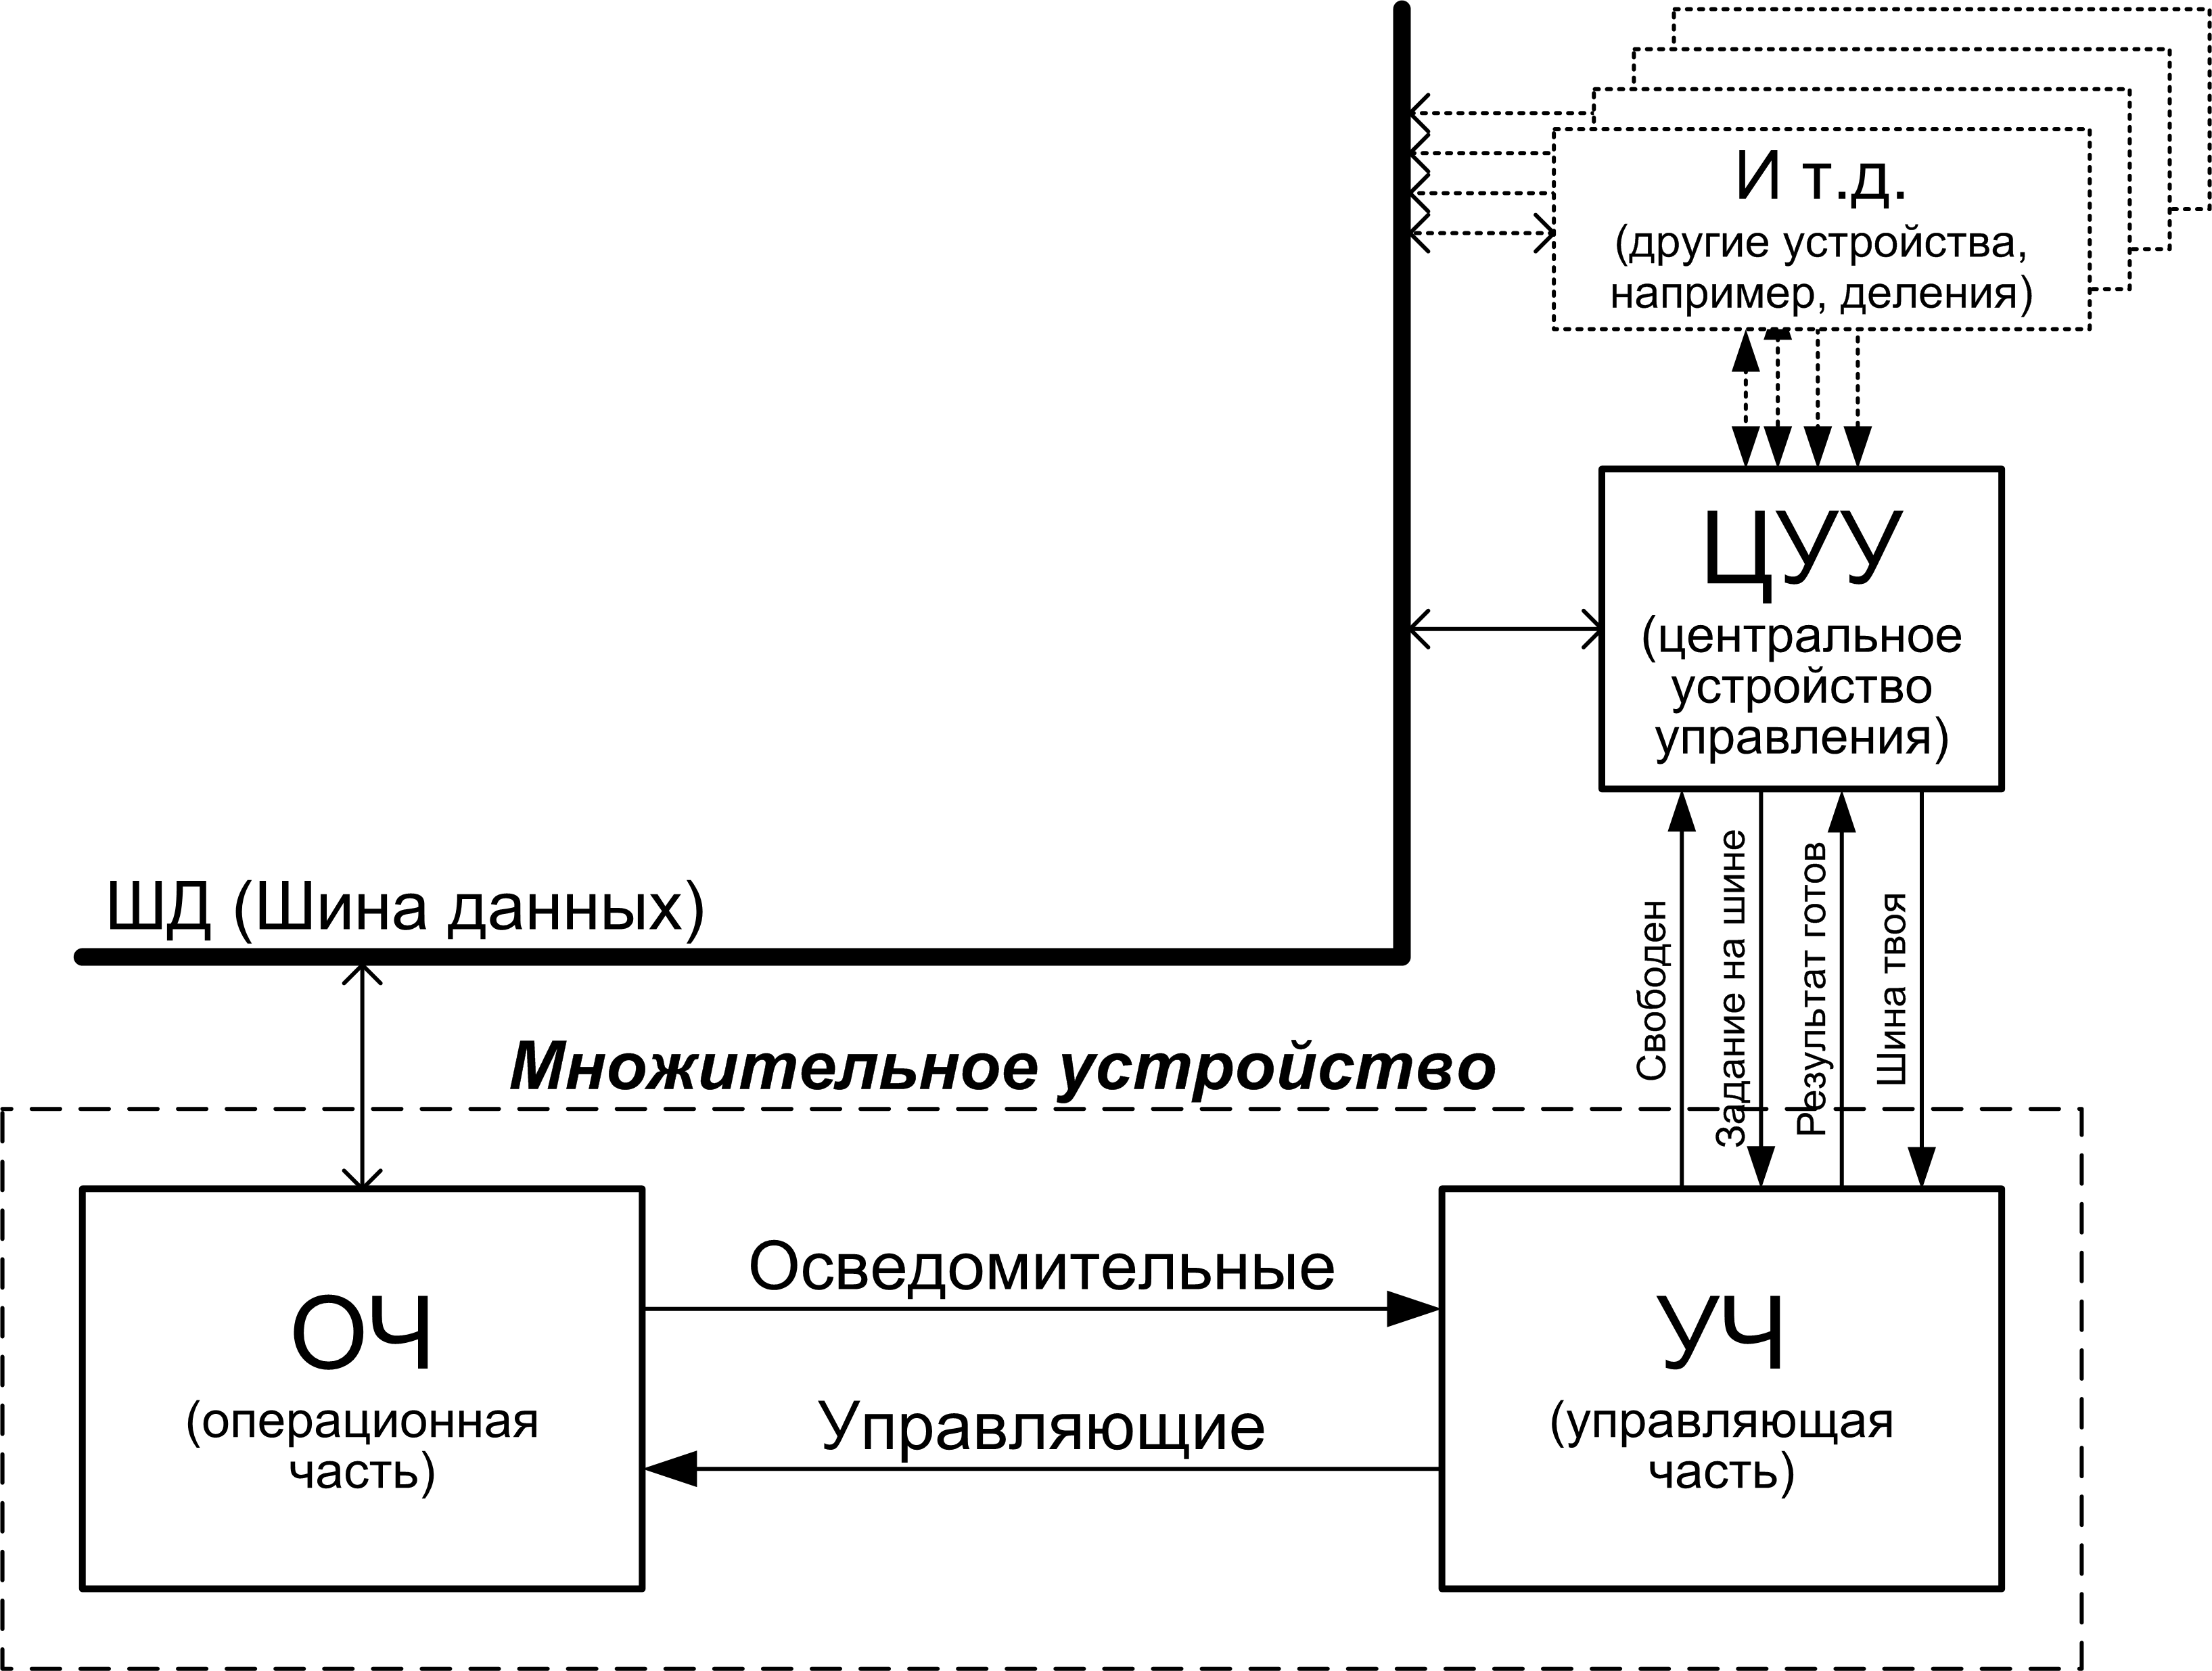
\includegraphics{fig/model}
    \caption{Структура вычислительного устройства}
    \label{fig::ch::practice::model}
\end{figure}

Структурно устройство разделяется на три компонента (см. рисунок \ref{fig::ch::practice::model}): 
\begin{itemize}
    \item центральное устройство управления (ЦУУ);
    \item операционная часть множительного устройства (ОЧ); 
    \item управляющая часть множетельного устройства (УЧ).
\end{itemize}

ЦУУ выполняет \emph{программу} пользователя, состоящую из отдельных \emph{команд}. Одной из команд является команда выполнить умножение. ЦУУ не выполняет эту операцию самсостоятельно, а дает задание множительному устройству. Множительное устройство, состоящее из операционной (ОЧ) и управляющей частей (УЧ), является лишь одним из многих устройств, которым ЦУУ перепоручает выполнить сложые операции.

Операция умножения, например, сводится к последовательности операций сложения, которые являются элементарными. Все остальные сложные операции также сводятся к выполнению элементарных операций по определенному алгоритму. \emph{Элементарная} операция выполняется некоторым элементом оборудования\footnote{Например, сложение выполняется логической схемой --- сумматором. См. описание этого элемента в разделе \ref{s::ch::practice::elements}} операционной части (ОЧ) сразу, за фиксированный (и относительно короткий) промежуток времени, называемый \emph{тактом}. В составе любого цифрового устройства имеется таймер, отсчитывающий такты\footnote{Отсюда термин \emph{тактовая частота}: $1/T$, где $T$ --- продолжительность такта}. Поэтому, когда говорится <<сложная операция>>, то подразумевается операция, выполняемая за несколько тактов.

При отсутствии сбоев, между центральным управляющим устройством (ЦУУ) и управляющей частью множительного устройства (УЧ) происходит следующий обмен синалами и данными:
\begin{enumerate}
    \item \textbf{УЧ$\to$ЦУУ:<<Свободен>>}. 
    
    УЧ выдает сигнал в ЦУУ <<Свободен>> всегда, когда не выполняет задачу. Отсутствие сигнала <<Свободен>> от УЧ трактуется ЦУУ как признак того, что множительное устройство занято решением ранее поставленной задачи.
    
    \item \textbf{ЦУУ$\to$УЧ:<<Задание на шине>>, ШД=<<Операнды>>}.

    Убедившись, что множительное устройство готово принять задание (получив от УЧ сигнал <<Свободен>>), ЦУУ выдает в УЧ сигнал <<Задание на шине>>. Передача задания по шине в общем случае может занять один или несколько тактов. Это зависит от принятых соглашений на формат передачи задания --- в общем случае это серия передач по шине данных. Получив сигнал <<Задание на шине>>, УЧ должна в следующем такте снять сигнал <<Свободен>>, и одновременно начать считывать с шины первый фрагмент задания.
    
    \item \textbf{УЧ$\to$ЦУУ:<<Результат готов>>}. 
    
    УЧ с помощью ОЧ выполняет умножение. Этот процесс может длиться довольно долго, и в это время ЦУУ может декодировать следующую команду и, если это возможно, начать её выполнять параллельно с работой мнжительного устройства. Так как при этом по шине данных (ШД) могут передаваться данные, получив результат, УЧ не должно выдавать его на шину сразу. УЧ выдает в ЦУУ осведомительный сигнал <<Результат готов>> и держит его до тех пор, пока ЦУУ не освободит шину.
    
    \item \textbf{ЦУУ$\to$УЧ:<<Шина твоя>>}. 
    
    ЦУУ, получив от УЧ сигнал <<Результат готов>>: завершает (если шина занята) текущую передачу данных по шине; выдает сигнал в УЧ <<Шина твоя>> и снимает его в следующем такте.
    
    \item \textbf{УЧ$\to$ЦУУ:ШД=<<Результат>>}. 
    
    Получив от ЦУУ сигнал <<Шина твоя>>, УЧ следующем такте должна:
    \begin{itemize}
        \item снять сигнал <<Результат готов>>;
        \item выдать на шину первый фрагмент результата, и если необходимо, продолжить в следующих тактах выдачу остальных фрагментов результата.
    \end{itemize}
\end{enumerate}

УЧ множительного устройства, выполняя алгоритм умножения, в каждом такте выдает в ОЧ необходимые управляющие сигналы. Управляющие сигналы формируются УЧ в зависимости от своего внутреннего состояния и осведомительных сигналов, часть которых поступает из ОЧ, а часть из ЦУУ. Аппаратура ОЧ содержит набор необходимых утройств, чтобы выполнить все необходимые элементарные операции.

ОЧ составлена из базовых схемотехнических цифровых элементов: логических элементов, сумматоров, мультиплексоров, триггеров, регистров, операционных усилителей и т.д. Необходимые сведения о работе этих элементов приводятся в разделе \ref{s::ch::practice::elements}.

%пришел ребенок и написал "зцуекнка Сахар словарное слово. рампмика аемпитьтлпаолдююююмпимпмвччвроолпеаакгогрипрппннпрпагшпенучвчаер"

\section{Элементы функциональной схемы}
\label{s::ch::practice::elements}

В данном разделе приводится необходимый минимум сведений для изображения и понимания функциональных схем. За исчерпывающей информацией обращайтесь к стандарту \cite{bib:gost:fs}.


\subsection{Сигналы, шины, жгуты}


Отдельная \emph{сигнальная линия} соответствует проводнику (проводу), который передает логические значения 0 или 1. Сигнальная линия на схеме изображается тонкой линией, соедняющей выход некоторого элемента со входом некоторого элемента. 

Множество внешних (интерфейсных) сигнальных линий принято объединять в \emph{шины}. Шина на схеме изображается толстой линией и обязательно именуется: сверху над линией в удобном месте подписывается имя шины (на рисунке \ref{fig::ch::practice::bus} изображена шина $X$). В общем случае шин на схеме может быть несколько. В качестве имени шины обычно выбирают заглавную литеру: $X$, $Y$, $Z$, $P$, а если шины разделены по функциональному назначению, то они могут быть названы: ШД --- шина данных, ША --- шина адреса, ШУ --- шина управления и т.д.

\begin{figure}[!ht]
    \centering
    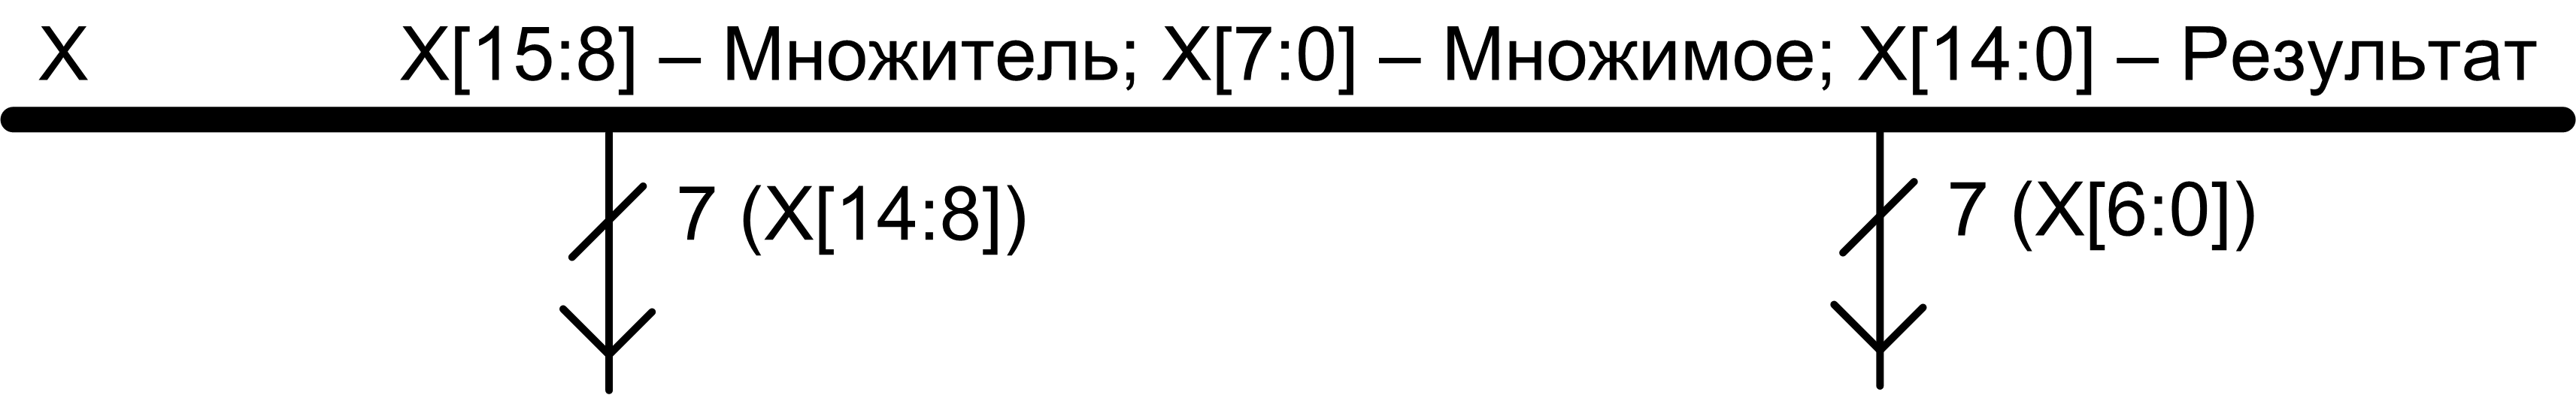
\includegraphics{fig/bus}
    \caption{Изображение шин и жгутов}
    \label{fig::ch::practice::bus}
\end{figure}

Чтобы не рисовать множество параллельных сигнальных линий, в случае, когда передается группа бит, на схеме изображают \emph{жгут}. Жгут также изображается тонкой линией, на которой в произвольном месте (но не на концах) тонкими линиями рисуется тупоугольная стрелка, указвающая направление передачи, сверху от стрелки жгут перечеркивается косой чертой и справа указывается разрядность жгута. В случае когда требуется указать, какие разряды шины отведены в жгут, в скобках после разрядности перечисляются обозначения групп сигнальных линий в составе шины. На рисунке \ref{fig::ch::practice::bus} от шины $X$ отведены два жгута по $7$ разрядов каждый.

\emph{Сигналы} разделяют на осведомительные и управляющие. Управляющие сигналы обычно обозначаются: $Y0$, $Y1$, $Y2$,\ldots, а осведомительные --- $P0$, $P1$, $P2$,\ldots Если управляющий сигнал подается на вход элемента, а не на управление, то стрелку не рисуют.  На рисунке \ref{fig::ch::practice::controls} изображен $8$-и разрядный регистр (подробнее о регистрах см. раздел \ref{sss::ch::practice::regiter}), который управляется сигналами $Y0$, $Y1$. Седьмой разряд выхода регистра используется как осведомительный сигнал $P0$. На входные разряды с $0$ по $3$ подаются соответственно сигналы с $3$ по $6$ шины $X$. На вход $RG1[7:4]$ подается двоичное значение $(0011)_2$.

Управляющие сигналы подводятся стрелками, входящими в управляемый блок справа. Осведомительные отводятся с выходов стрелкой, направленной вниз или влево.

\begin{figure}[!ht]
    \centering
    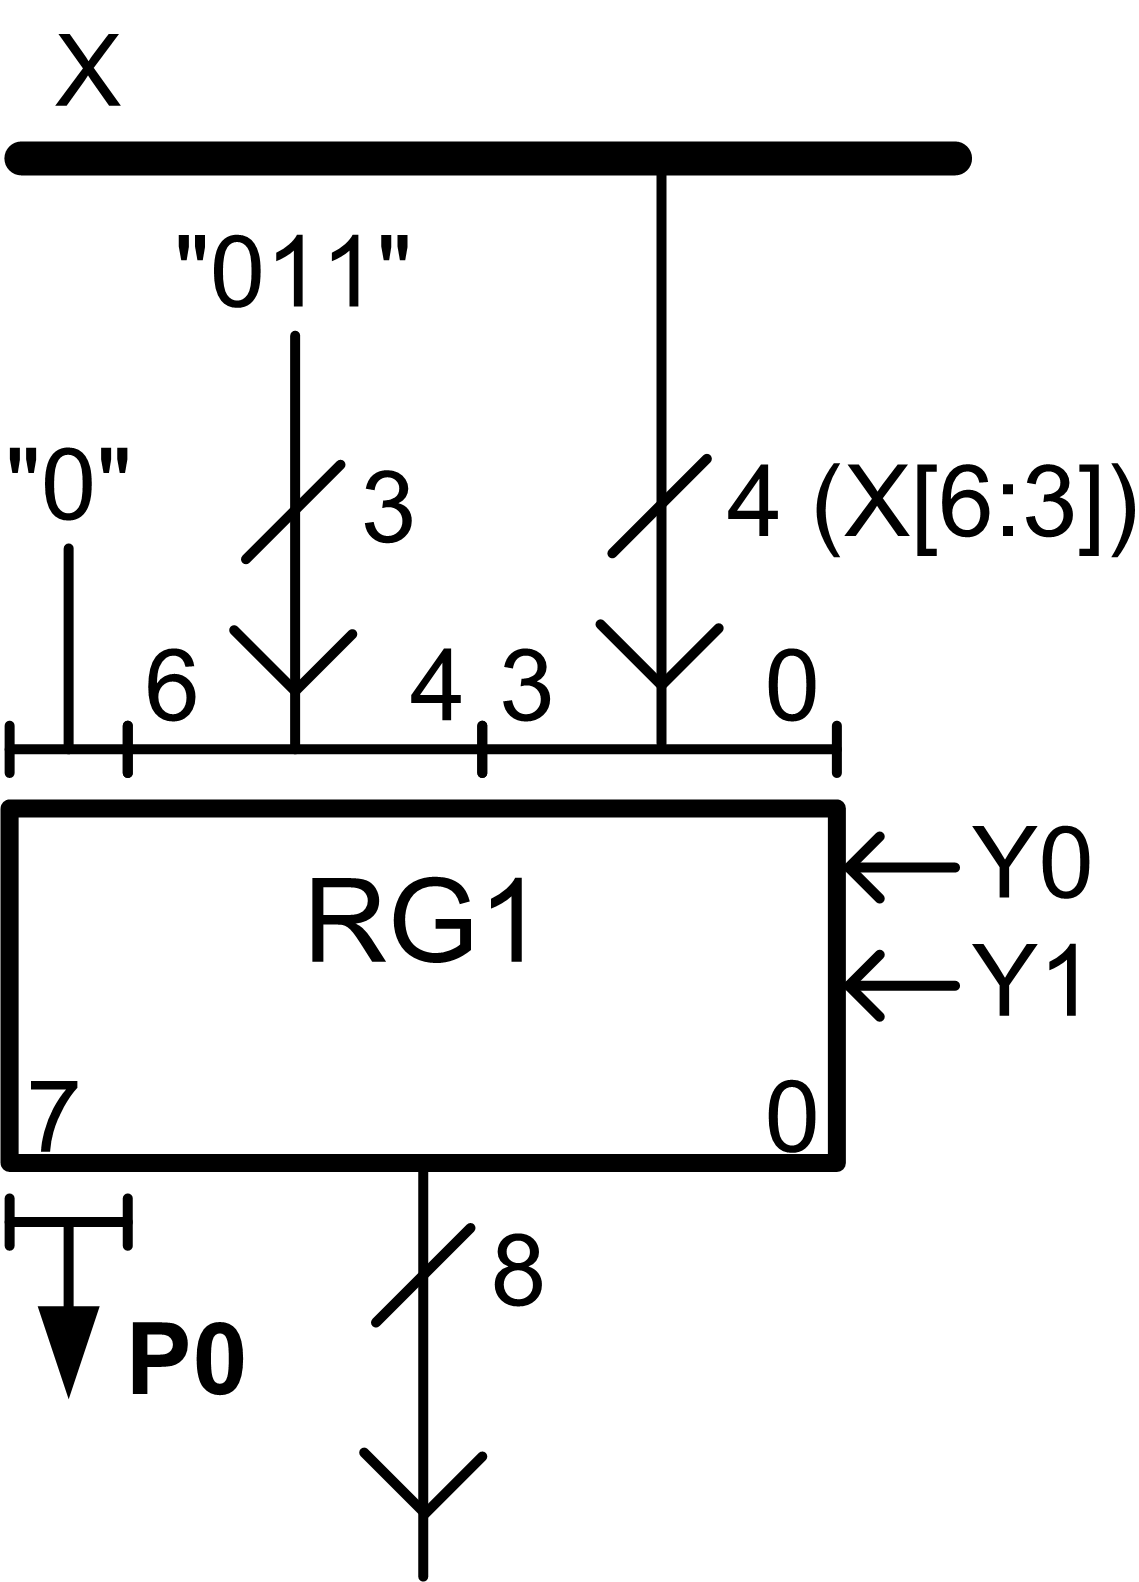
\includegraphics{fig/controls}
    \caption{Входы, выходы и управляющие сигналы регистра}
    \label{fig::ch::practice::controls}
\end{figure}

\begin{figure}[!ht]
    \centering
    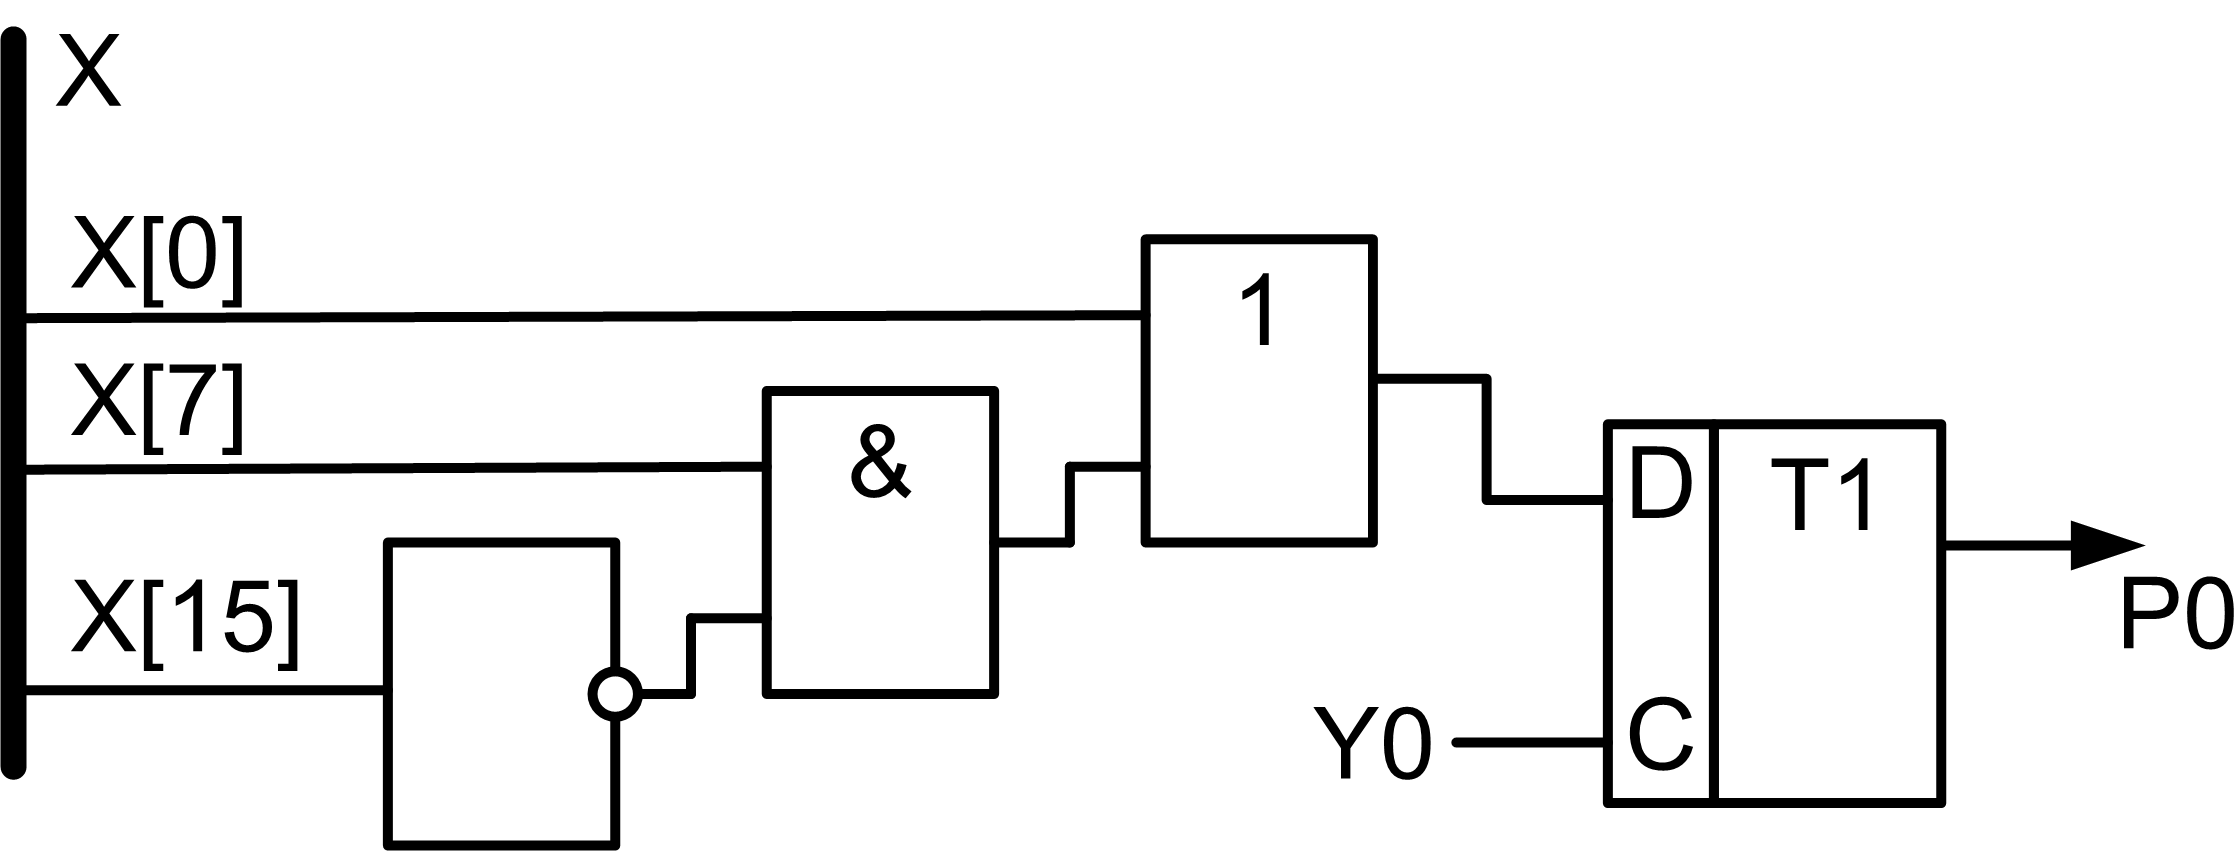
\includegraphics{fig/logic}
    \caption{Логическая схема}
    \label{fig::ch::practice::logic}
\end{figure}

Входы большинства элементов на схеме подводятся сверху, а выходы --- снизу. Исключением являются элементы логической схемы и триггеры (см. рисунок \ref{fig::ch::practice::logic}), в которой входы подаются слева, а выходы снимаются справа. В любом случае недопустимо разворачивать или переворачивать блоки.

Если о разрядности входов можно судить по разрядности выходов, то допустимо подписывать только разрядности выходов элементов.


\subsection{Элементы логики}

Элементы логики отличаются от элементов памяти тем, что представляют собой реализацию однотактной функции: выход формируется за один такт времени и зависит только от информации на входах. У элементов логики нет внутреннего состояния. Типичные элементы логики это: логические схемы (И, ИЛИ, НЕ, XOR, И-НЕ, и т.д.), мультиплексоры, сумматоры, шинные формирователи и т.д.


\subsubsection{Многовходовые логические функции}

На схемах элементы, реализующие многовходовую ассоциативную и комутативную логическую функцию (И, ИЛИ, XOR), допустимо изображать одним элементом, как на рисунке \ref{fig::ch::practice::bigLogic}.
\begin{figure}[!ht]
    \centering
    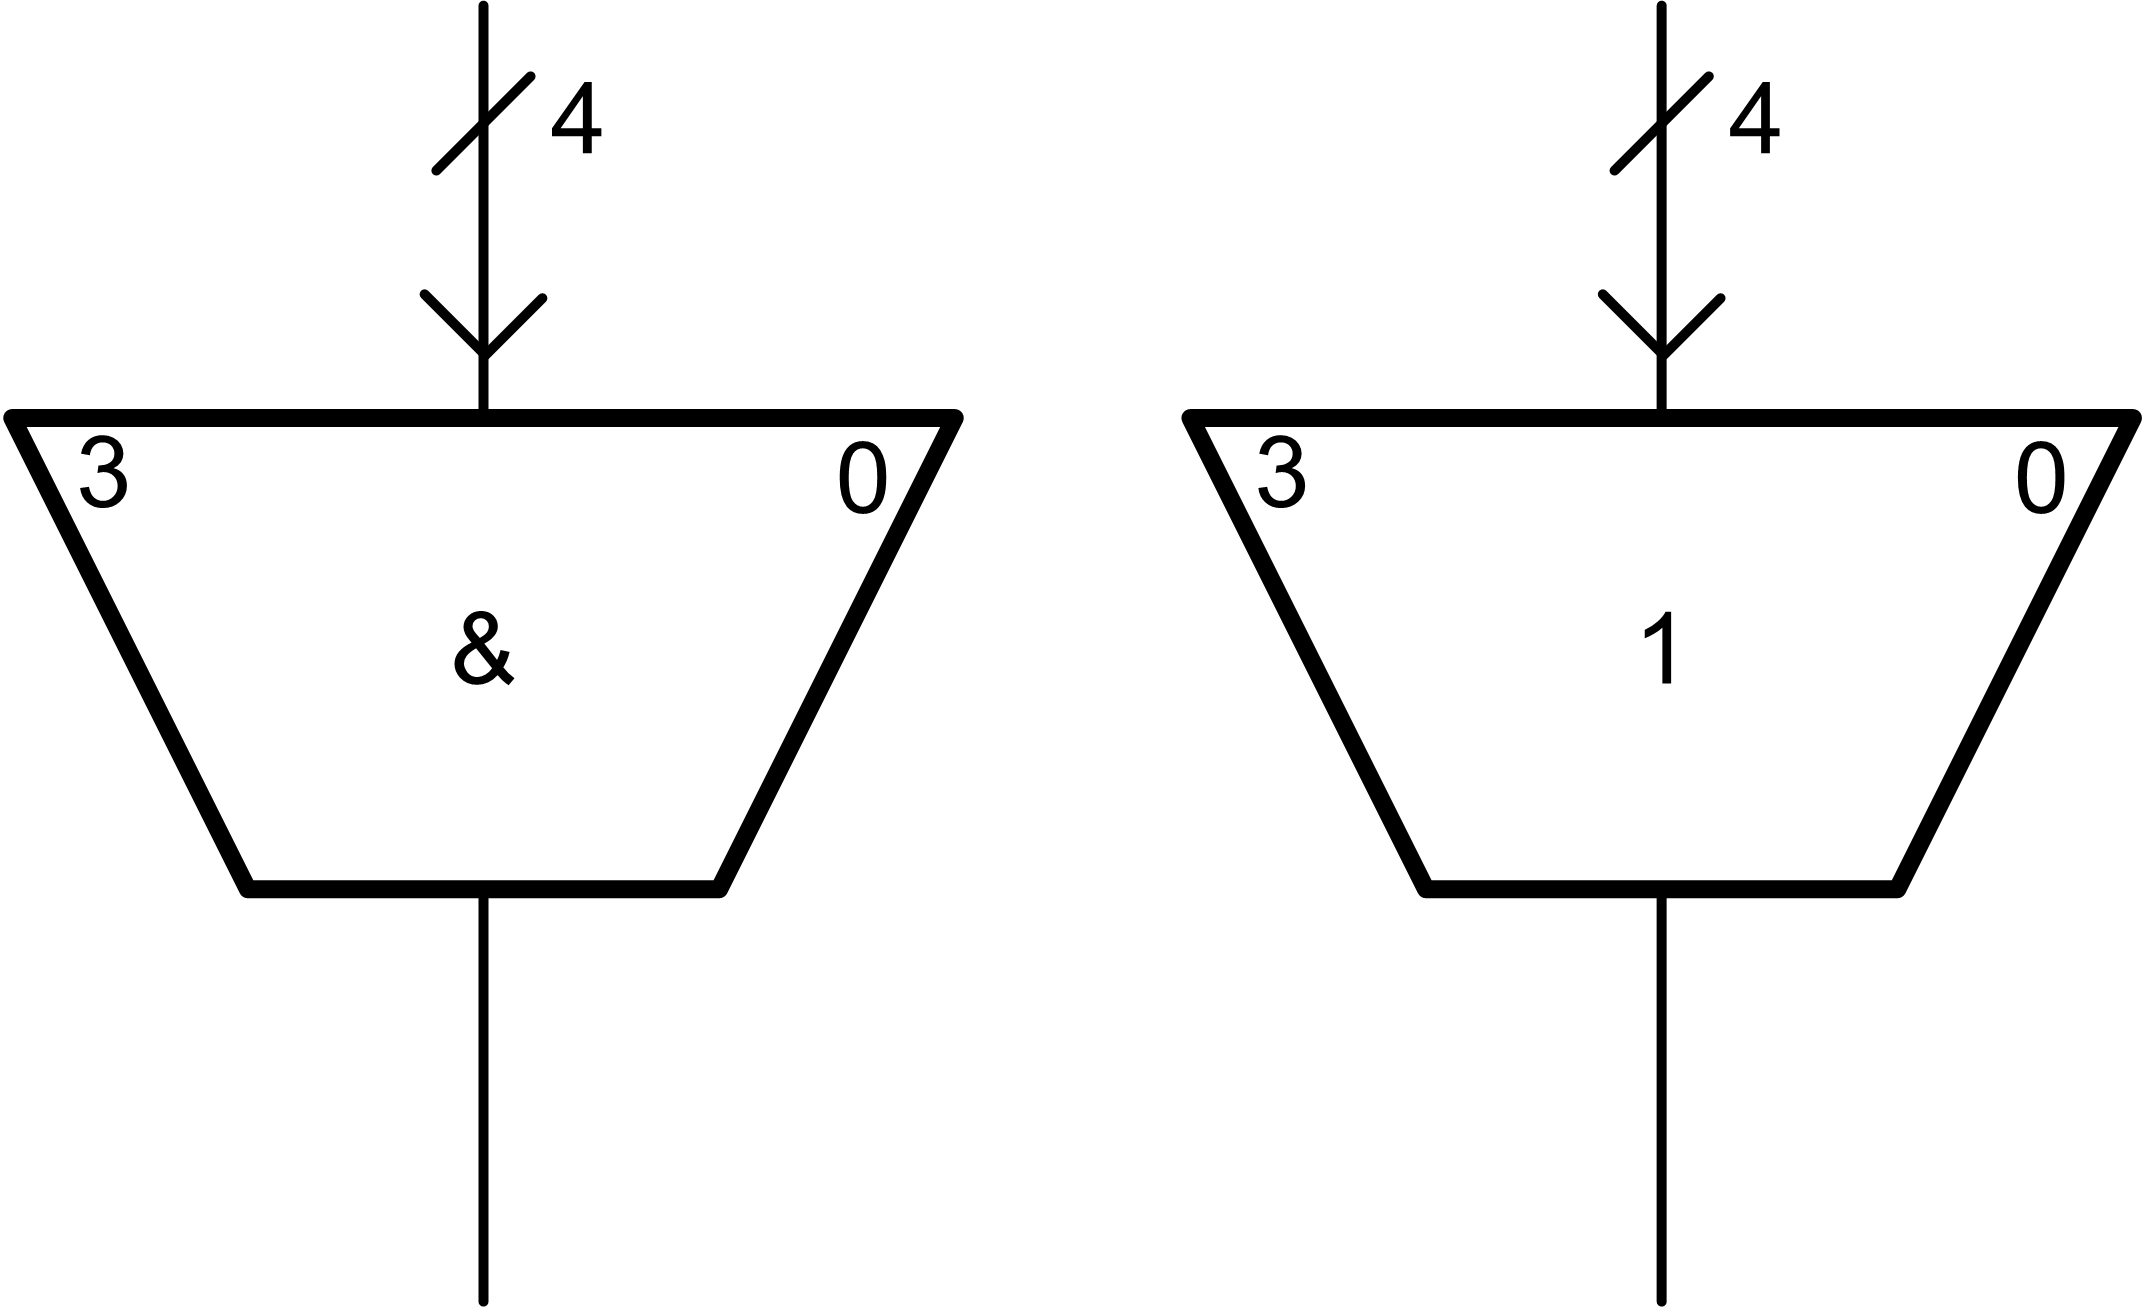
\includegraphics{fig/bigLogic}
    \caption{$4$-х входовые функции И, ИЛИ}
    \label{fig::ch::practice::bigLogic}
\end{figure}

Выход такого элемента --- одноразрядный.


\subsubsection{Инвертор}

На схемах многоразрядный инвертор изображается как рисунке \ref{fig::ch::practice::invertor}.
\begin{figure}[!ht]
    \centering
    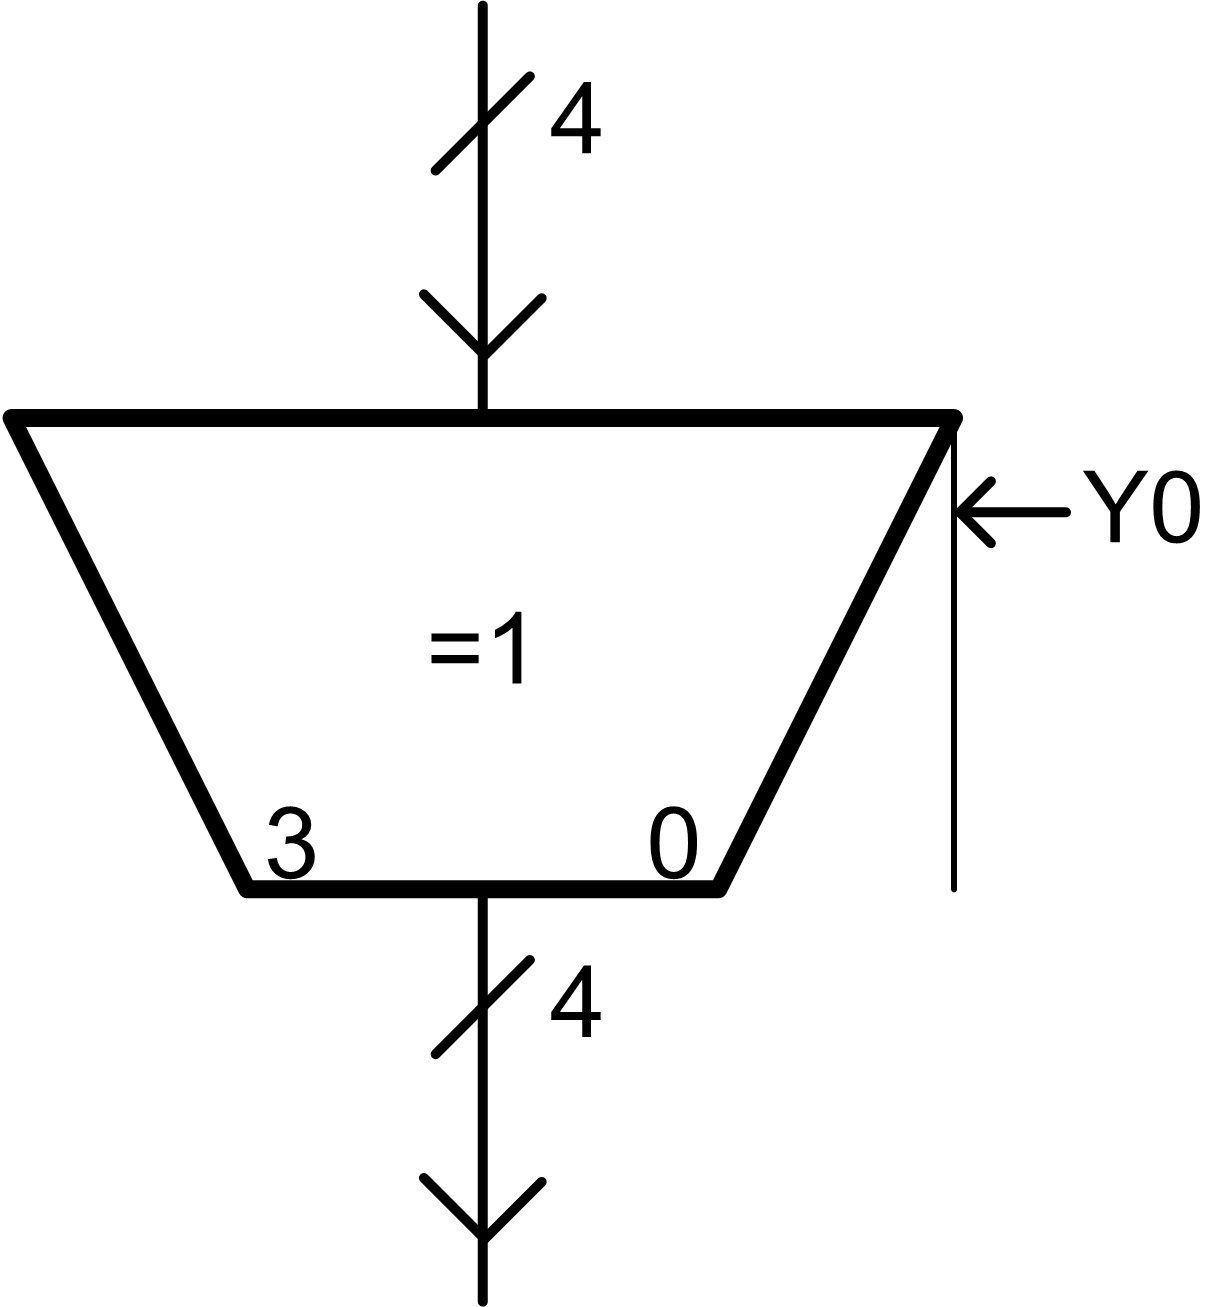
\includegraphics{fig/invertor}
    \caption{$4$-х разрядный инвертор}
    \label{fig::ch::practice::invertor}
\end{figure}

Если значение единственного управляющего сигнала 0, то разряды входа без изменений подаются на выход, иначе на выходе формируется поразрядная инверсия входа.

\subsubsection{Мультиплексор}

Условное графическое обозначение мультиплексора приведено на рисунке \ref{fig::ch::practice::mux}.
\begin{figure}[!ht]
    \centering
    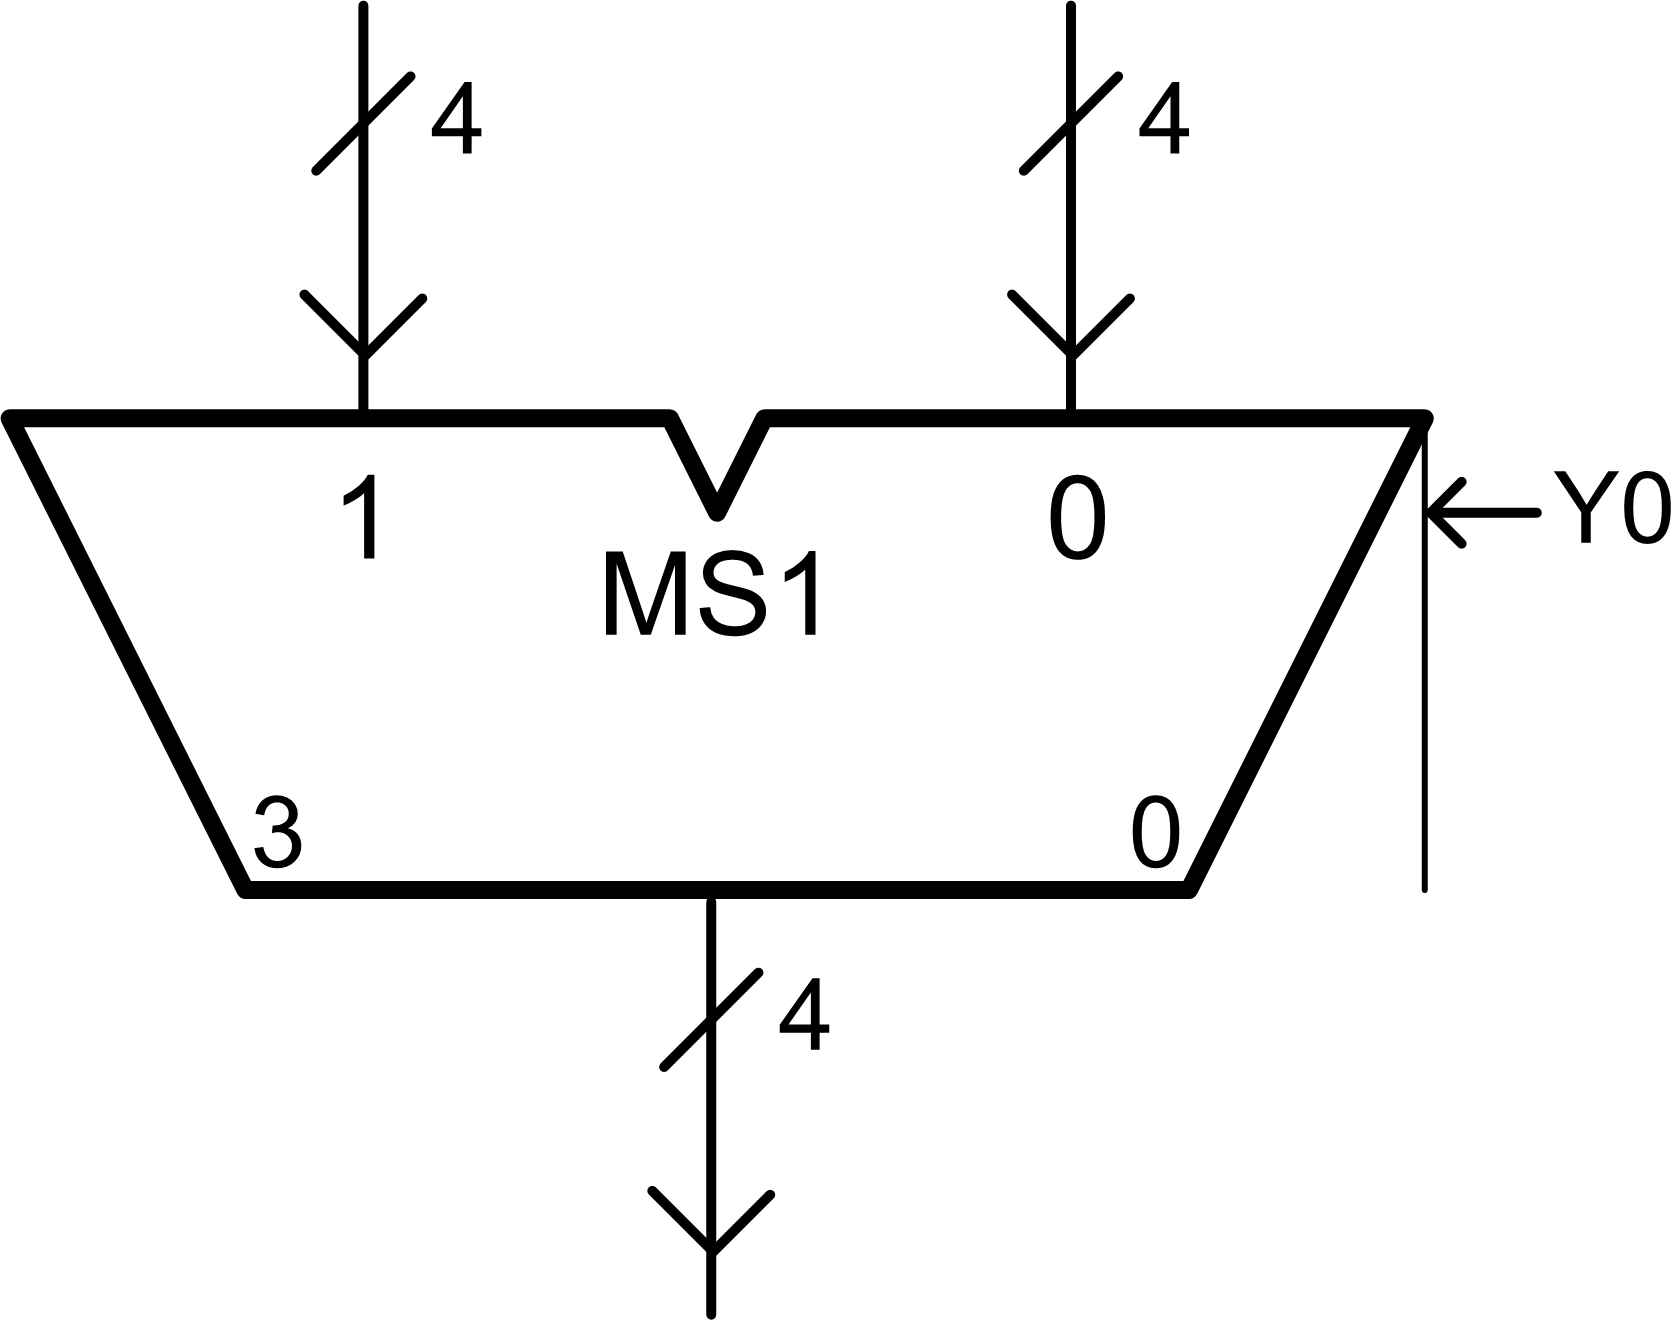
\includegraphics{fig/mux}
    \caption{Мультиплексор}
    \label{fig::ch::practice::mux}
\end{figure}

В зависимости от значения управляющего сиграла (на рисунке \ref{fig::ch::practice::mux} это $Y0$) на выход подается либо нулевое, либо первое входное плечо.

Мультиплексоры с большим количеством плеч могут быть получены на основе $2$-плечевых мультиплексоров каскадным подключением. Мультиплексор с произвольным количеством плеч рисуют упрощенно (см. рисунок \ref{fig::ch::practice::muxbig}). При этом самый верхний управляющий сигнал соответствует младшему разряду (LSB\footnote{LSB --- Least Significant Bit, Младший бит}) двоичного представления номера плеча, а самый нижний - старшему (MSB\footnote{MSB --- Most Significant Bit, Старший бит}). Например, чтобы выбрать 2-е плечо мультиплексора на рисунке \ref{fig::ch::practice::muxbig} нужно подать $Y1=1$, $Y0=0$.

\begin{figure}[!ht]
    \centering
    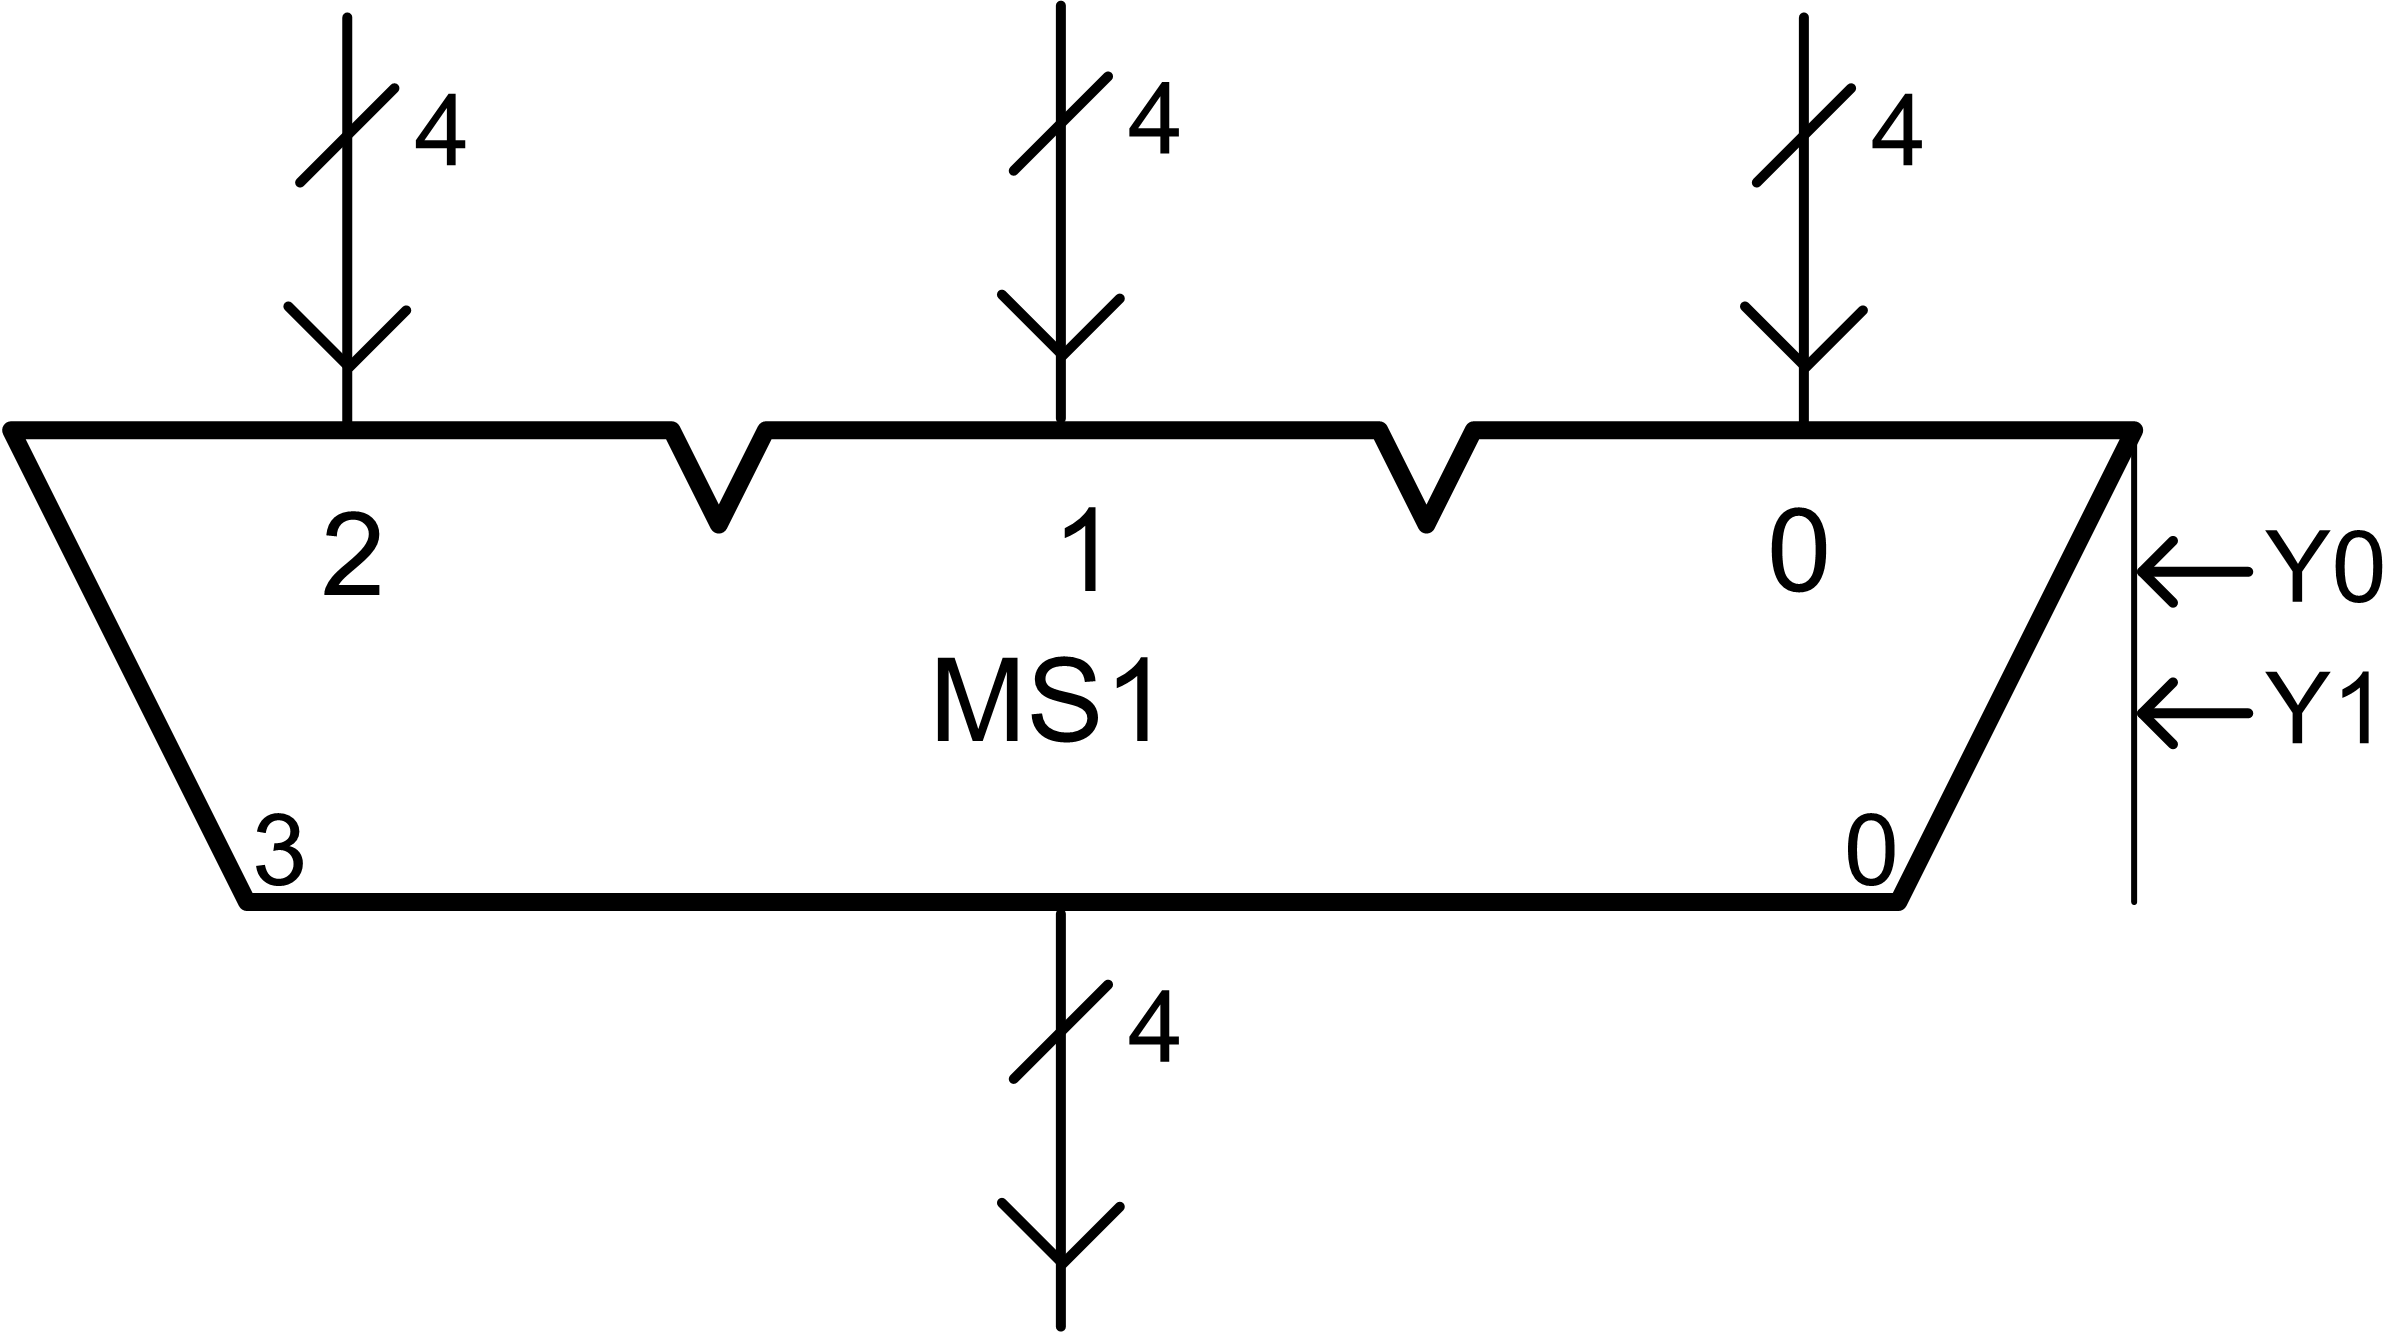
\includegraphics{fig/muxbig}
    \caption{Многоплечевой мультиплексор}
    \label{fig::ch::practice::muxbig}
\end{figure}


\subsubsection{Сумматор}

Условное графическое обозначение сумматора приведено на рисунке \ref{fig::ch::practice::summator}.
\begin{figure}[!ht]
    \centering
    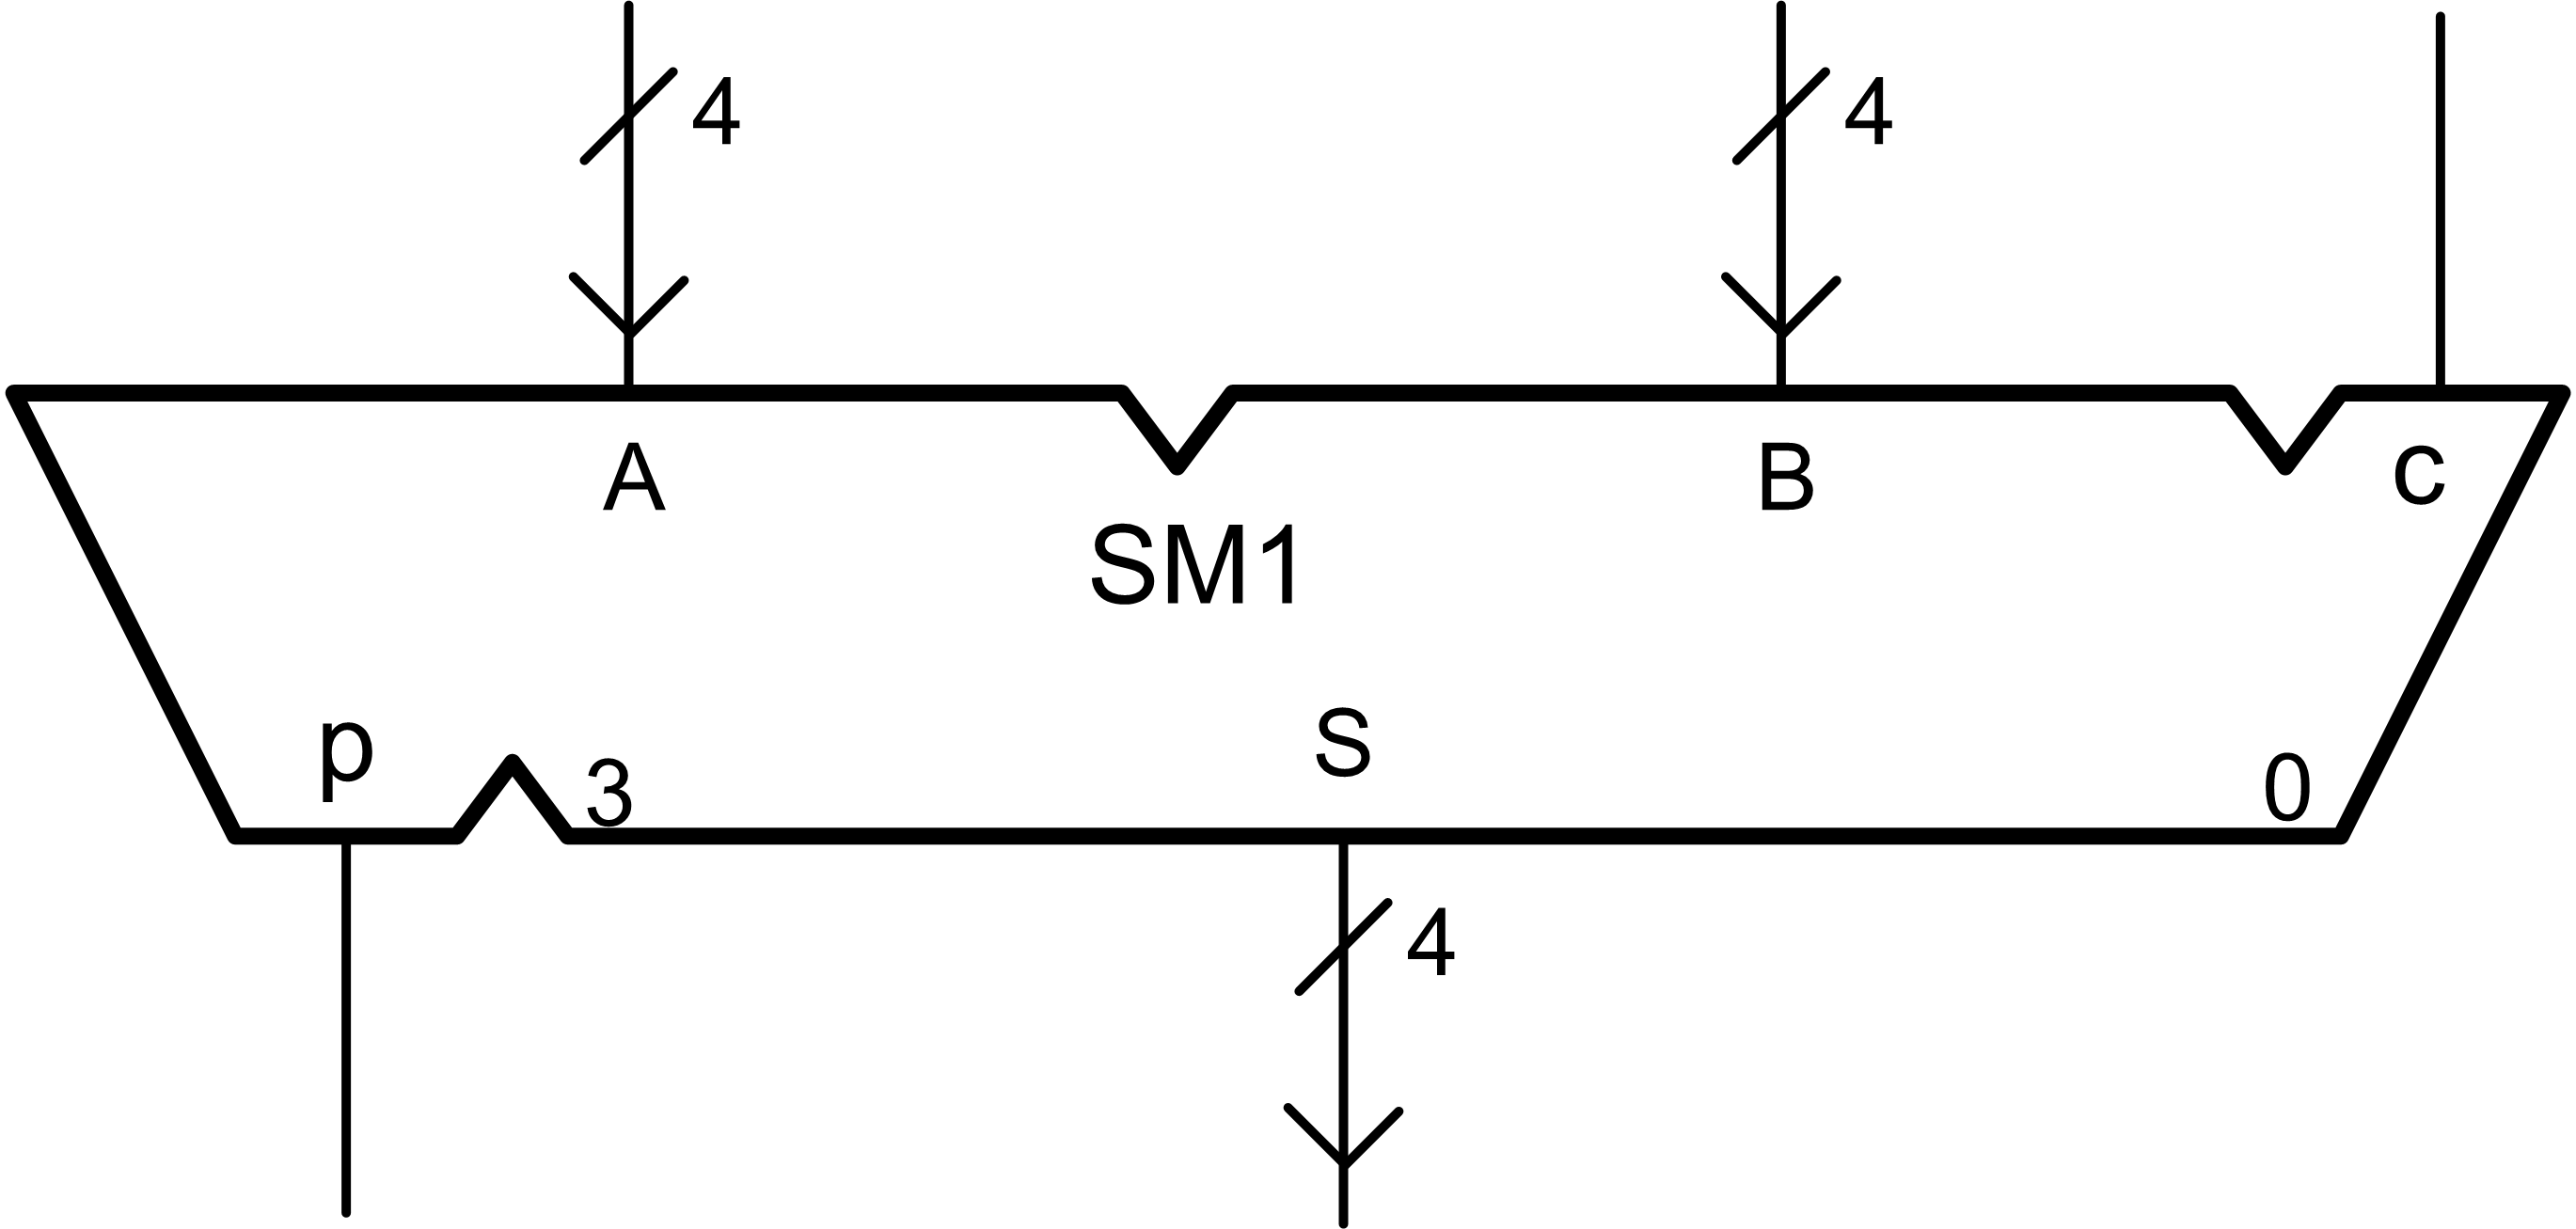
\includegraphics{fig/summator}
    \caption{Сумматор}
    \label{fig::ch::practice::summator}
\end{figure}

Сумматор выполняет арифметическое сложение $n$-разрядных входов (на рисунке \ref{fig::ch::practice::summator} $n=4$) входов $A$ и $B$ а также одноразрядного входа переноса в младшие разряды $c$. На выход $S$ выдаются младшие $n$ разрядов результата, а на выход $p$ --- бит переноса из старшего $(n-1)$-го разряда суммы $S$:
\begin{align*}
    S \equiv (A + B + c) \pmod{2^n};\\
    p = (A + B + c) \div{2^n}.
\end{align*}

В случае, если нужно получить сумматор большей разрядности на основе сумматоров меньшей разрядности, то выход переноса из старших разрядов младшего сумматора замыкают на вход переноса старшего сумматора (см. рисунок \ref{fig::ch::practice::summators}).
\begin{figure}[!ht]
    \centering
    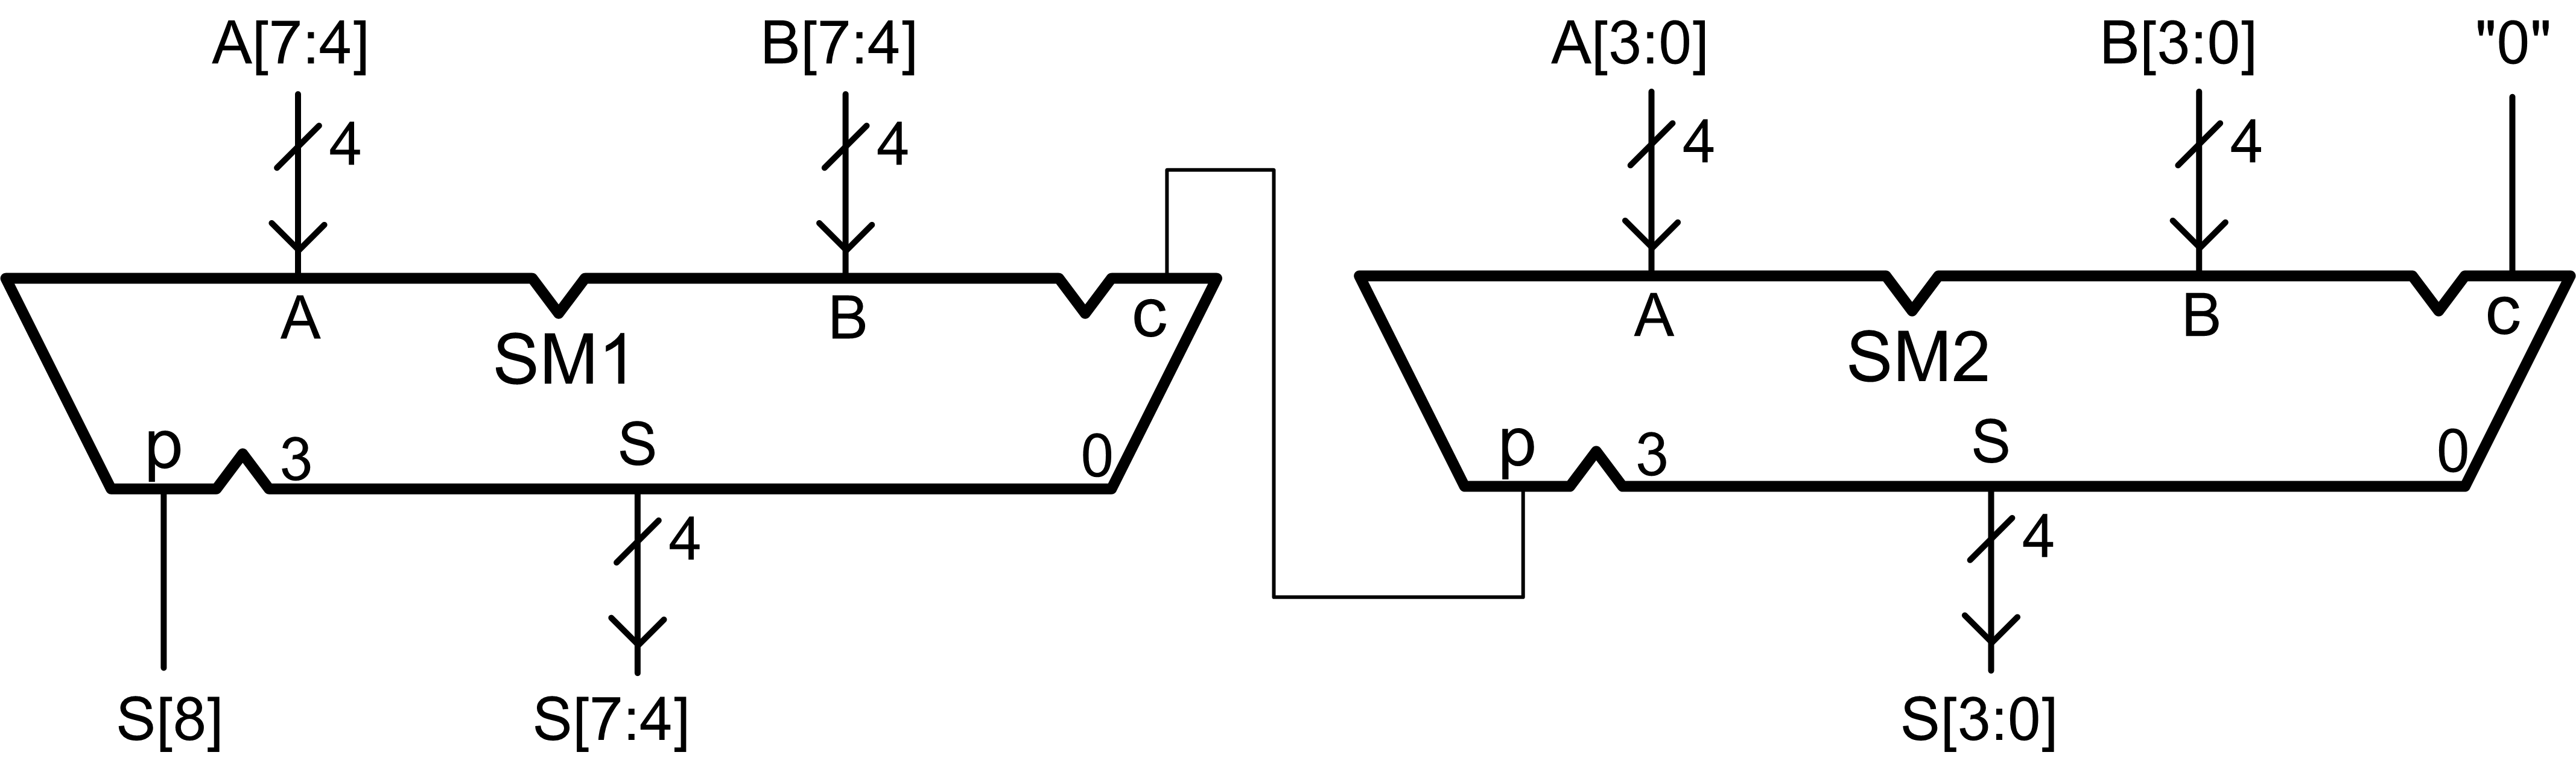
\includegraphics[width=.85\textwidth]{fig/summators}
    \caption{8-разрядный сумматор на основе двух 4-х разрядных}
    \label{fig::ch::practice::summators}
\end{figure}

На схемах сумматор любой разрядности рисуют одним элементом, если неважно, как этот сумматор устроен.


\subsubsection{Шинный формирователь}

Шинным формирователем устройство называется потому, что обычно его выходы подключены к шине. По управляюещму сигналу (на рисунке \ref{fig::ch::practice::zbuffer} сигнал $Y0$) шинный формирователь может отключать свои выходы от шины. Когда шинный формирователь подключен к шине, он выдает данные со входа на шину. Так как шина может быть общей для нескольких устройств, то использование шинных формирователей обязательно, чтобы гарантировать, что только одно устройство выдает на шину данные.

\begin{figure}[!ht]
    \centering
    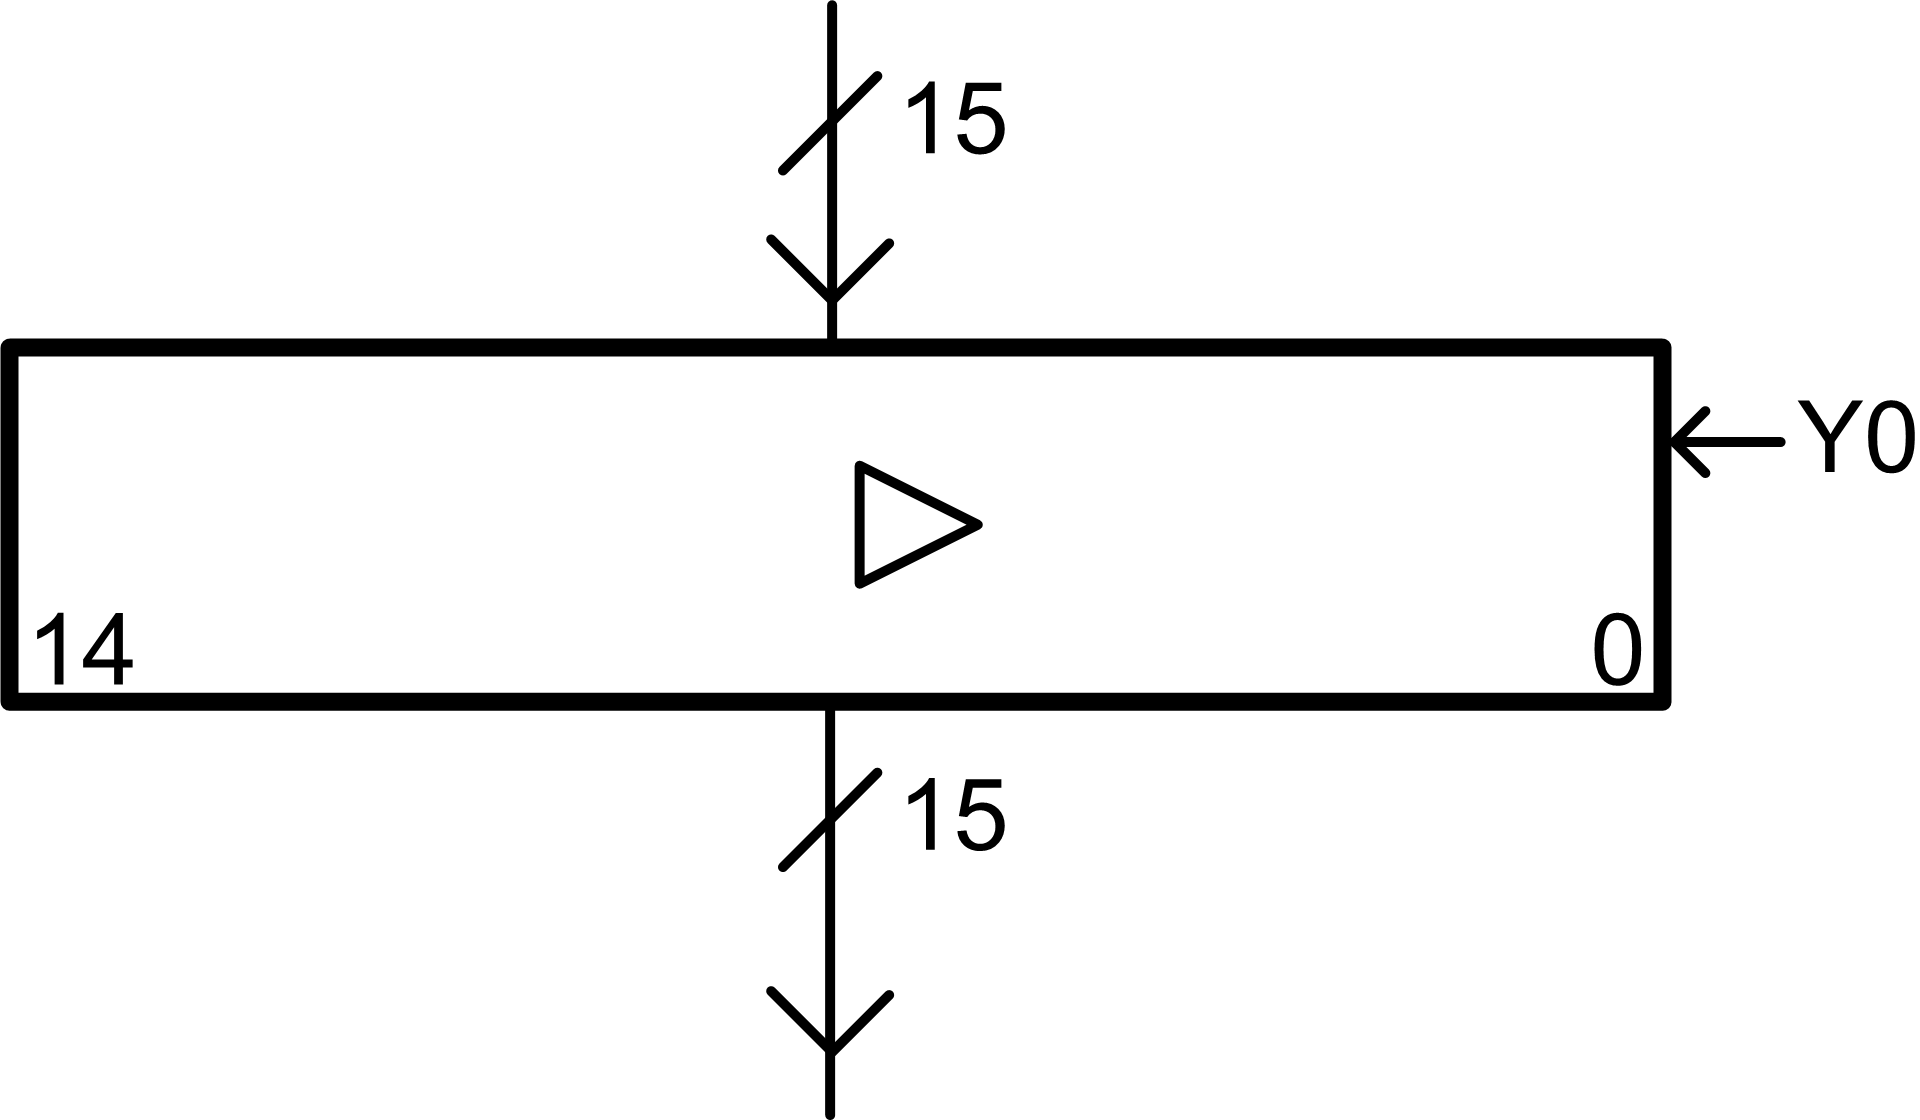
\includegraphics{fig/zbuffer}
    \caption{15-разрядный шинный формирователь}
    \label{fig::ch::practice::zbuffer}
\end{figure}


\subsection{Элементы памяти}

Элементы памяти могут сохрянять информацию (состояние) между тактами. Они обычно имеют управляющий сигнал, который управляет запоминанием информации со входов. Т.е. в течение такта такой элемент либо <<запоминает>> информацию со входов, либо хранит (или преобразует) ранее запомненную информацию.

\subsubsection{Регистры}
\label{sss::ch::practice::regiter}

Обычный регистр содержит автономную $n$-разрядную ячейку памяти и предназначен только для запоминания $n$ бит информации со входов. Помимо основной функции он может, например, выполнить сброс всех бит своей ячейки памяти в $0$ или $1$. На выходы регистра всегда выдается содержимое его внутренней ячейки памяти.

\begin{figure}[!ht]
    \centering
    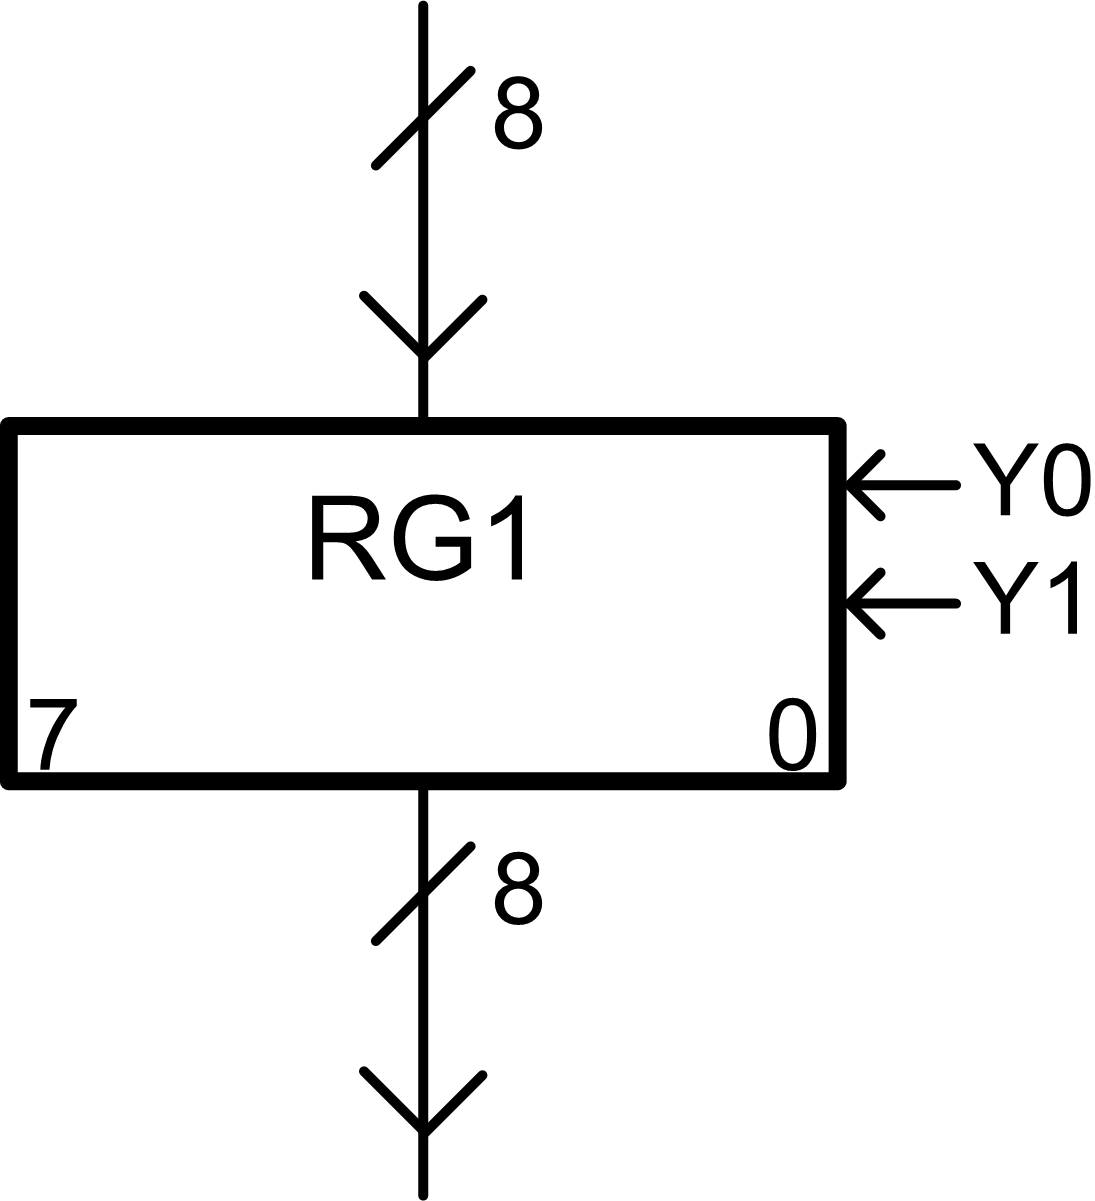
\includegraphics{fig/register}
    \caption{8-разрядный регистр}
    \label{fig::ch::practice::register}
\end{figure}

Например, на рисунке \ref{fig::ch::practice::register} изображен обычный регистр, расшифровка управляющих сигналов которого может быть следующей:
\begin{itemize}
    \item $Y0$ --- разрешение записи в $RG1$. Если данный сигнал подается в течение такта, то регистр <<запоминает>> информацию со входов и хранит до тех пор, пока $Y0$ вновь не будет подан в будущем.

    \item $Y1$ --- сброс всех разрядов внутренней ячейки памяти $RG1$ в $0$.
\end{itemize}

Управляющие сигналы регистра могут конфликтовать, например, состояние регистра не определено, если одновременно подать сигналы разрешения записи и сброса.

Сдвиговые регистры изображаются особым образом, в виде параллелограмма. Направление сдвига разрядов ячейки памяти обозначается стрелкой внутри регистра. Например, при сдвиге влево значение старшего разряда теряется, а в младший разряд заносится значение разряда со специального входа, который изображается боковой планкой с нужного края. 

\begin{figure}[!ht]
    \centering
    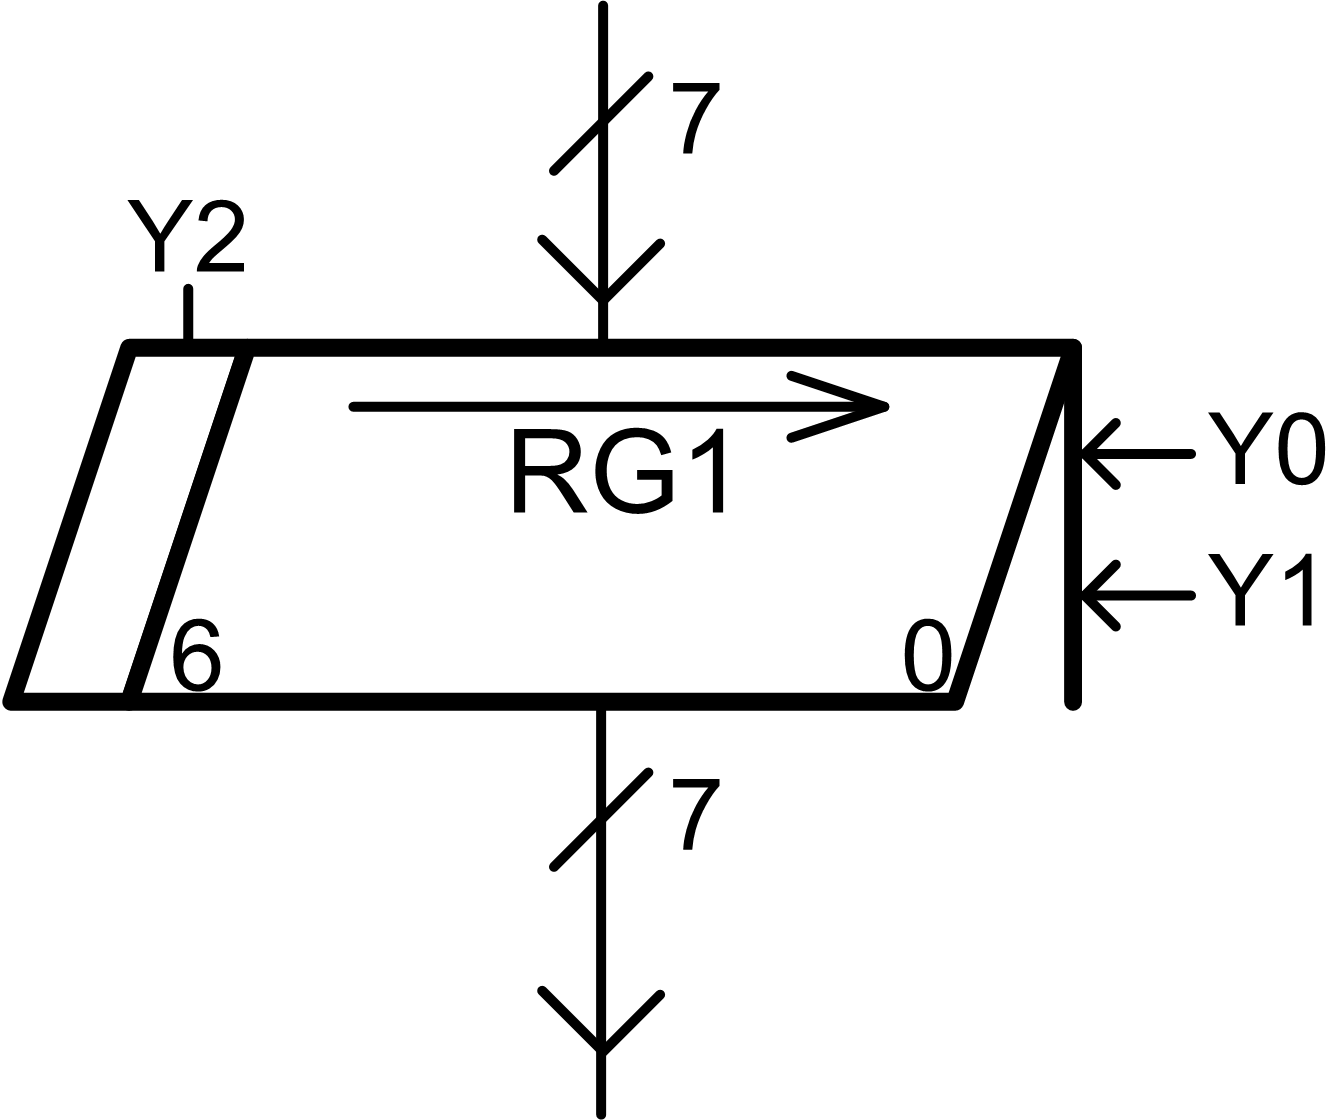
\includegraphics{fig/shiftregister}
    \caption{7-разрядный сдвиговый регистр}
    \label{fig::ch::practice::shiftregister}
\end{figure}

На рисунке \ref{fig::ch::practice::shiftregister} изображен сдвиговый регистр, расшифровка управляющих сигналов которого может быть следующей:
\begin{itemize}
    \item $Y0$ --- разрешение записи в $RG1$. Если данный сигнал подается в течение такта, то регистр <<запоминает>> информацию со входов и хранит до тех пор, пока $Y0$ вновь не будет подан в будущем.

    \item $Y1$ --- сдвиг $RG1$ вправо.
    
    \item вход $Y2$ определяет значение $6$-го разряда при сдвиге.
\end{itemize}


\subsubsection{Триггеры}

Триггер --- это одноразрядное запоминающее устройство. Триггеров существует несколько видов: D, RS, JK, \ldots В схемах будет использоваться D-триггер (см. рисунок \ref{fig::ch::practice::dtrigger}), который можно считать одноразрядным регистром: если на вход $C$ подается 1, то триггер <<запоминает>> бит информации со входа $D$, а если на вход $C$ подается 0, то триггер выдает ранее запомненный бит.

\begin{figure}[!ht]
    \centering
    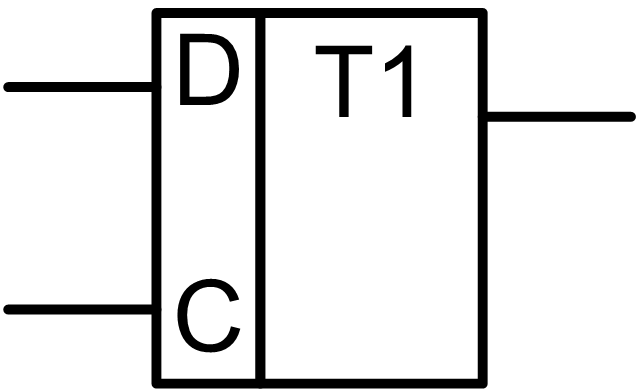
\includegraphics{fig/dtrigger}
    \caption{D-триггер}
    \label{fig::ch::practice::dtrigger}
\end{figure}

\section{Основы микропрограммного управления}
\label{ch::practice::programming}

Множительное устройство, ЦУУ и другие модули (см. рисунок \ref{fig::ch::practice::model}) работают автономно и каждый выполняет собственный алгоритм функционирования. Например, УЧ множительного устройства в бесконечном цикле выполняет алгоритм: принять задания от ЦУУ; выполнить умножение; выдать в ЦУУ результаты. ЦУУ, например, выполняет в бесконечном цикле алгоритм: считать очередную команду программы пользвателя из памяти; декодировать её; выдать необходимые задания исполнительным модулям; дождаться результатов, считать и сохранить их; выбрать следующую команду\ldots

УЧ модуля (в том числе и множительного устройства) представляет собой автомат, по тактам выполняющий алгоритм работы модуля. Существует несколько способов создания таких автоматов. В данном разделе будут рассморены математические основы функционирования управляющих автоматов, а затем особый вид таких автоматов --- \emph{микропрограммные}.

В математической основе выделяют два типа управляющих автоматов: автоматы Мили и автоматы Мура. Общим для автоматов обоих типов является:
\begin{itemize}
    \item Внутреннее состояние. Автомат в течение такта находится в одном из множества возможных внутренних состояний. По завершении такта, автомат переключается в новое состояние. Множество внутренних состояний 
    \[ 
        S=\{s_0,\ldots,s_{n-1}\}.
    \]
    
    \item Начальное состояние $s_0$. С этого внутреннего состояния автомат начинает свою работу.
    
    \item Набор значений (вектор) осведомительных сигналов
    \[
        P=(p_{m-1},\ldots,p_0).
    \]
	
	Новое внутреннее состояние, в которое перейдет автомат, определяется его текущим внутренним состоянием и значениями осведомительных сигналов, которые поступали ему в течение такта.
    
    
    \item Набор управляющих сигналов
    \[
        Y=(y_{k-1},\ldots,y_0).
    \]
	
	Автомат в течение такта формирует и выдает значения управляющих сигналов. В способе формирования  управляющих сигналов заключается главное отличие между автоматами Мили и Мура.
\end{itemize}

Если в $i$-м такте автомат находится в состоянии $s^{(i)}$, и поступают значения осведомительных сигналов $P^{(i)}$, то состояние $s^{(i+1)}$, в которое он перейдет в следующем такте, определяется функцией перехдов $\mathbf{S}$, а набор управляющих сигналов, которые выдаются в $i$-м такте $Y^{(i)}$ определяются функцией выходов $\mathbf{Y}$.

Для автомата Мили:
\begin{equation}
    \begin{aligned}
        s^{(i+1)}&=\mathbf{S}(s^{(i)}, P^{(i)});\\
        Y^{(i)}  &=\mathbf{Y}(s^{(i)}, P^{(i)}).
    \end{aligned}
    \label{eq::ch::practice::programming::Mili}
\end{equation}

Видно, что для автомата Мили векор управляющих сигналов $Y^{(i)}$ формируется на основе текущего состояния $s^{(i)}$ и вектора осведомительных сигналов $P^{(i)}$.

Для автомата Мура управляющие сигналы зависят только от текущего состояния:
\begin{equation}
    \begin{aligned}
        s^{(i+1)}&=\mathbf{S}(s^{(i)}, P^{(i)});\\
        Y^{(i)}  &=\mathbf{Y}(s^{(i)}).
    \end{aligned}
    \label{eq::ch::practice::programming::Moore}
\end{equation}

Работу автомата удобно изобразить на диаграмме переходов, которая представляет собой граф, вершинам которого соответствуют состояния, а дугам --- функция переходов $\mathbf{S}$. Начальное состояние $s_0$ обычно выделяется двойным контуром. Над дугой подписываются значения осведомительных сигналов, определяющих переход в следующее состояние. Так как управляющие сигналы в автомате Мили зависят от состояния автомата и осведомительных сигналов, то управляющими сигналами взвешиваются дуги. В автомате Мура управляющие сигналы зависят только от состояния, поэтому управляющими сигналами взвешиваются вершины.

Далее приводятся примеры диаграмм переходов автоматов, из раздела \ref{ss::ch::practice::software::example}, к этому разделу следует обратиться всем желающим понять назначение управляющих и осведомительных сигналов. Пока же --- это неважно.

\begin{figure}[!ht]
    \[
        {\xymatrix{
            *{}
                &*{}
                    &*{}
                        &s_3  \ar@{->}@/^/[dr]^(.3){*|\Machine{22h}} 
                            &*{}
                                &*{}
                                    &*{}
                                        &*{}
                                            \\
            *++[o][F=]{s_0}  \ar@{->}[r]^{p_0|\Machine{1h}}  \ar@{->}@(ur,ul)[]_{\bar{p}_0|\Machine{1h}}
                &s_1  \ar@{->}[r]^{*|\Machine{4h}}
                    &s_2  \ar@{->}[rr]^{\bar{p}_2|\Machine{12h}} \ar@{->}@/^/[ur]^{p_2|\Machine{18h}}
                        &*{}
                            &s_4  \ar@{->}[rr]^{p_1|\Machine{2h}} \ar@{->}@(r,u)[]_(.6){\bar{p}_1|\Machine{2h}}
                                &*{}
                                    &s_5  \ar@{->}@(d,d)[llllll]_{*|\Machine{41h}}
        }}
    \]
    \caption{Диаграмма переходов автомата Мили}
    \label{fig::ch::practice::MiliDiagram}
\end{figure}

На рисунке \ref{fig::ch::practice::MiliDiagram} приведена диаграмма автомата Мили. Далее приводится описание нескольких переходов.
\begin{itemize}
    \item Из начального состояния $s_0$, автомат переходит в состояние $s_1$, при $p_0=1$ (на схеме это обозначено как $p_0$); при этом выдается управляющий сигнал $y_0$ (на схеме вектор управляющих сигналов закодирован в 16-ичной СС: \Machine{1h}).
    
    \item Автомат остается в начальном состояниии если $\bar{p}_0$, при этом также выдается $y_0$.

    \item Из $s_1$ осуществляется переход только в $s_2$ --- осведомительные сигналы не важны (переход помечен $*$), при этом выдается управляющий сигнал $y_2$ (вектор \Machine{4h}).
    
    \item Из $s_5$ автомат безусловно возвращается в $s_0$ и выдает при этом набор сигналов $\{y_6,y_0\}$, т.е. вектор \Machine{41h}.
\end{itemize}

Из состояния $s_1$ автомат переходит только в состояние $s_2$, при этом значения осведомительных сигналов не важны и обозначены на схеме $*$, выдается управляющий сигнал $y_0$. И т.д.

\begin{figure}[!ht]
    \[
        {\xymatrix{
            *{} &*{}&*{}&*{}&*{}&*{}&*{}    \\
            *{}
                &*{}
                    &*{}
                        &s_5|\Machine{10h}    \ar@{->}@/^/[rrd]^{*} 
                            &*{}
                                &*{}
                                    &*{}
                                        \\
            *++[o][F=]{s_0|\Machine{1h}}  \ar@{->}[r]^{p_0}  \ar@{->}@(ur,ul)[]_{\bar{p}_0}
                &s_1|\Machine{4h}  \ar@{->}[r]^{*}
                    &s_2|\Machine{0h}  \ar@{->}[r]^{p_2}  \ar@{->}@/^/[ru]^{\bar{p}_2}
                        &s_3|\Machine{18h}  \ar@{->}[r]^{*}
                            &s_4|\Machine{20h}  \ar@{->}[r]^{*}
                                &s_6|\Machine{2h}  \ar@{->}[r]^{p_1} \ar@{->}@(ur,ul)[]_{\bar{p}_1}
                                    &s_7|\Machine{41h} \ar`d[dl]`_u[llllll]_{\bar{p}_0}[llllll]
                                                       \ar`u[uul]`[lllll]_{p_0}[lllll]
                                        %\ar@{->}@(d,d)[llllll]_{\bar{p}_0} \ar@{->}@(u,u)[lllll]_{p_0}
                                            \\
            *{} &*{}&*{}&*{}&*{}&*{}&*{}    \\
        }}
    \]
    \caption{Диаграмма переходов автомата Мура}
    \label{fig::ch::practice::MooreDiagram}
\end{figure}

На рисунке \ref{fig::ch::practice::MooreDiagram} приведена диаграмма автомата Мура. Далее следует описания нескольких переходов автомата.
\begin{itemize}
    \item Находясь в начальном состоянии, автомат выдает управлающий сигнал $y_0$ (вектор \Machine{1h}). Если выполняется условие $\bar{p}_0$, т.е. $p_0=0$, то автомат остается в начальном состоянии, в противном случае --- переходит в $s_1$.
    
    \item Из состояния $s_3$, в котором автомат выдает управляющие сигналы $\{y_4,y_3\}$, автомат безусловно переходит в $s_4$.
    
    \item Из состояния $s_5$ автомат может вернуться в начальное состояние или выполнить переход в $s_0$.
\end{itemize}

\emph{Микропрограммный} автомат в своем составе имеет два элемента --- микропроцессор и память \emph{микрокоманд}. Такие автоматы довольно удобны в обращении, так как позволяют задать алгоритм своей работы простой записью микропрограммы в память микрокоманд. Микрокоманда выполняется за один такт и сопровождается выдачей соответствующих управляющих сигналов.


\subsection{Микропрограммные автоматы}

Структура микропрограммного автомата Мили представлена на рисунке\footnote{Мы намеренно отступили от некоторых правил оформления схем --- например, мультиплексор MS1 в нашей схеме перевернут, а управление на MS2 подается слева} \ref{fig::ch::practice::Mili}, а Мура --- на рисунке \ref{fig::ch::practice::Moore}. 

\begin{figure}[!ht]
    \centering
    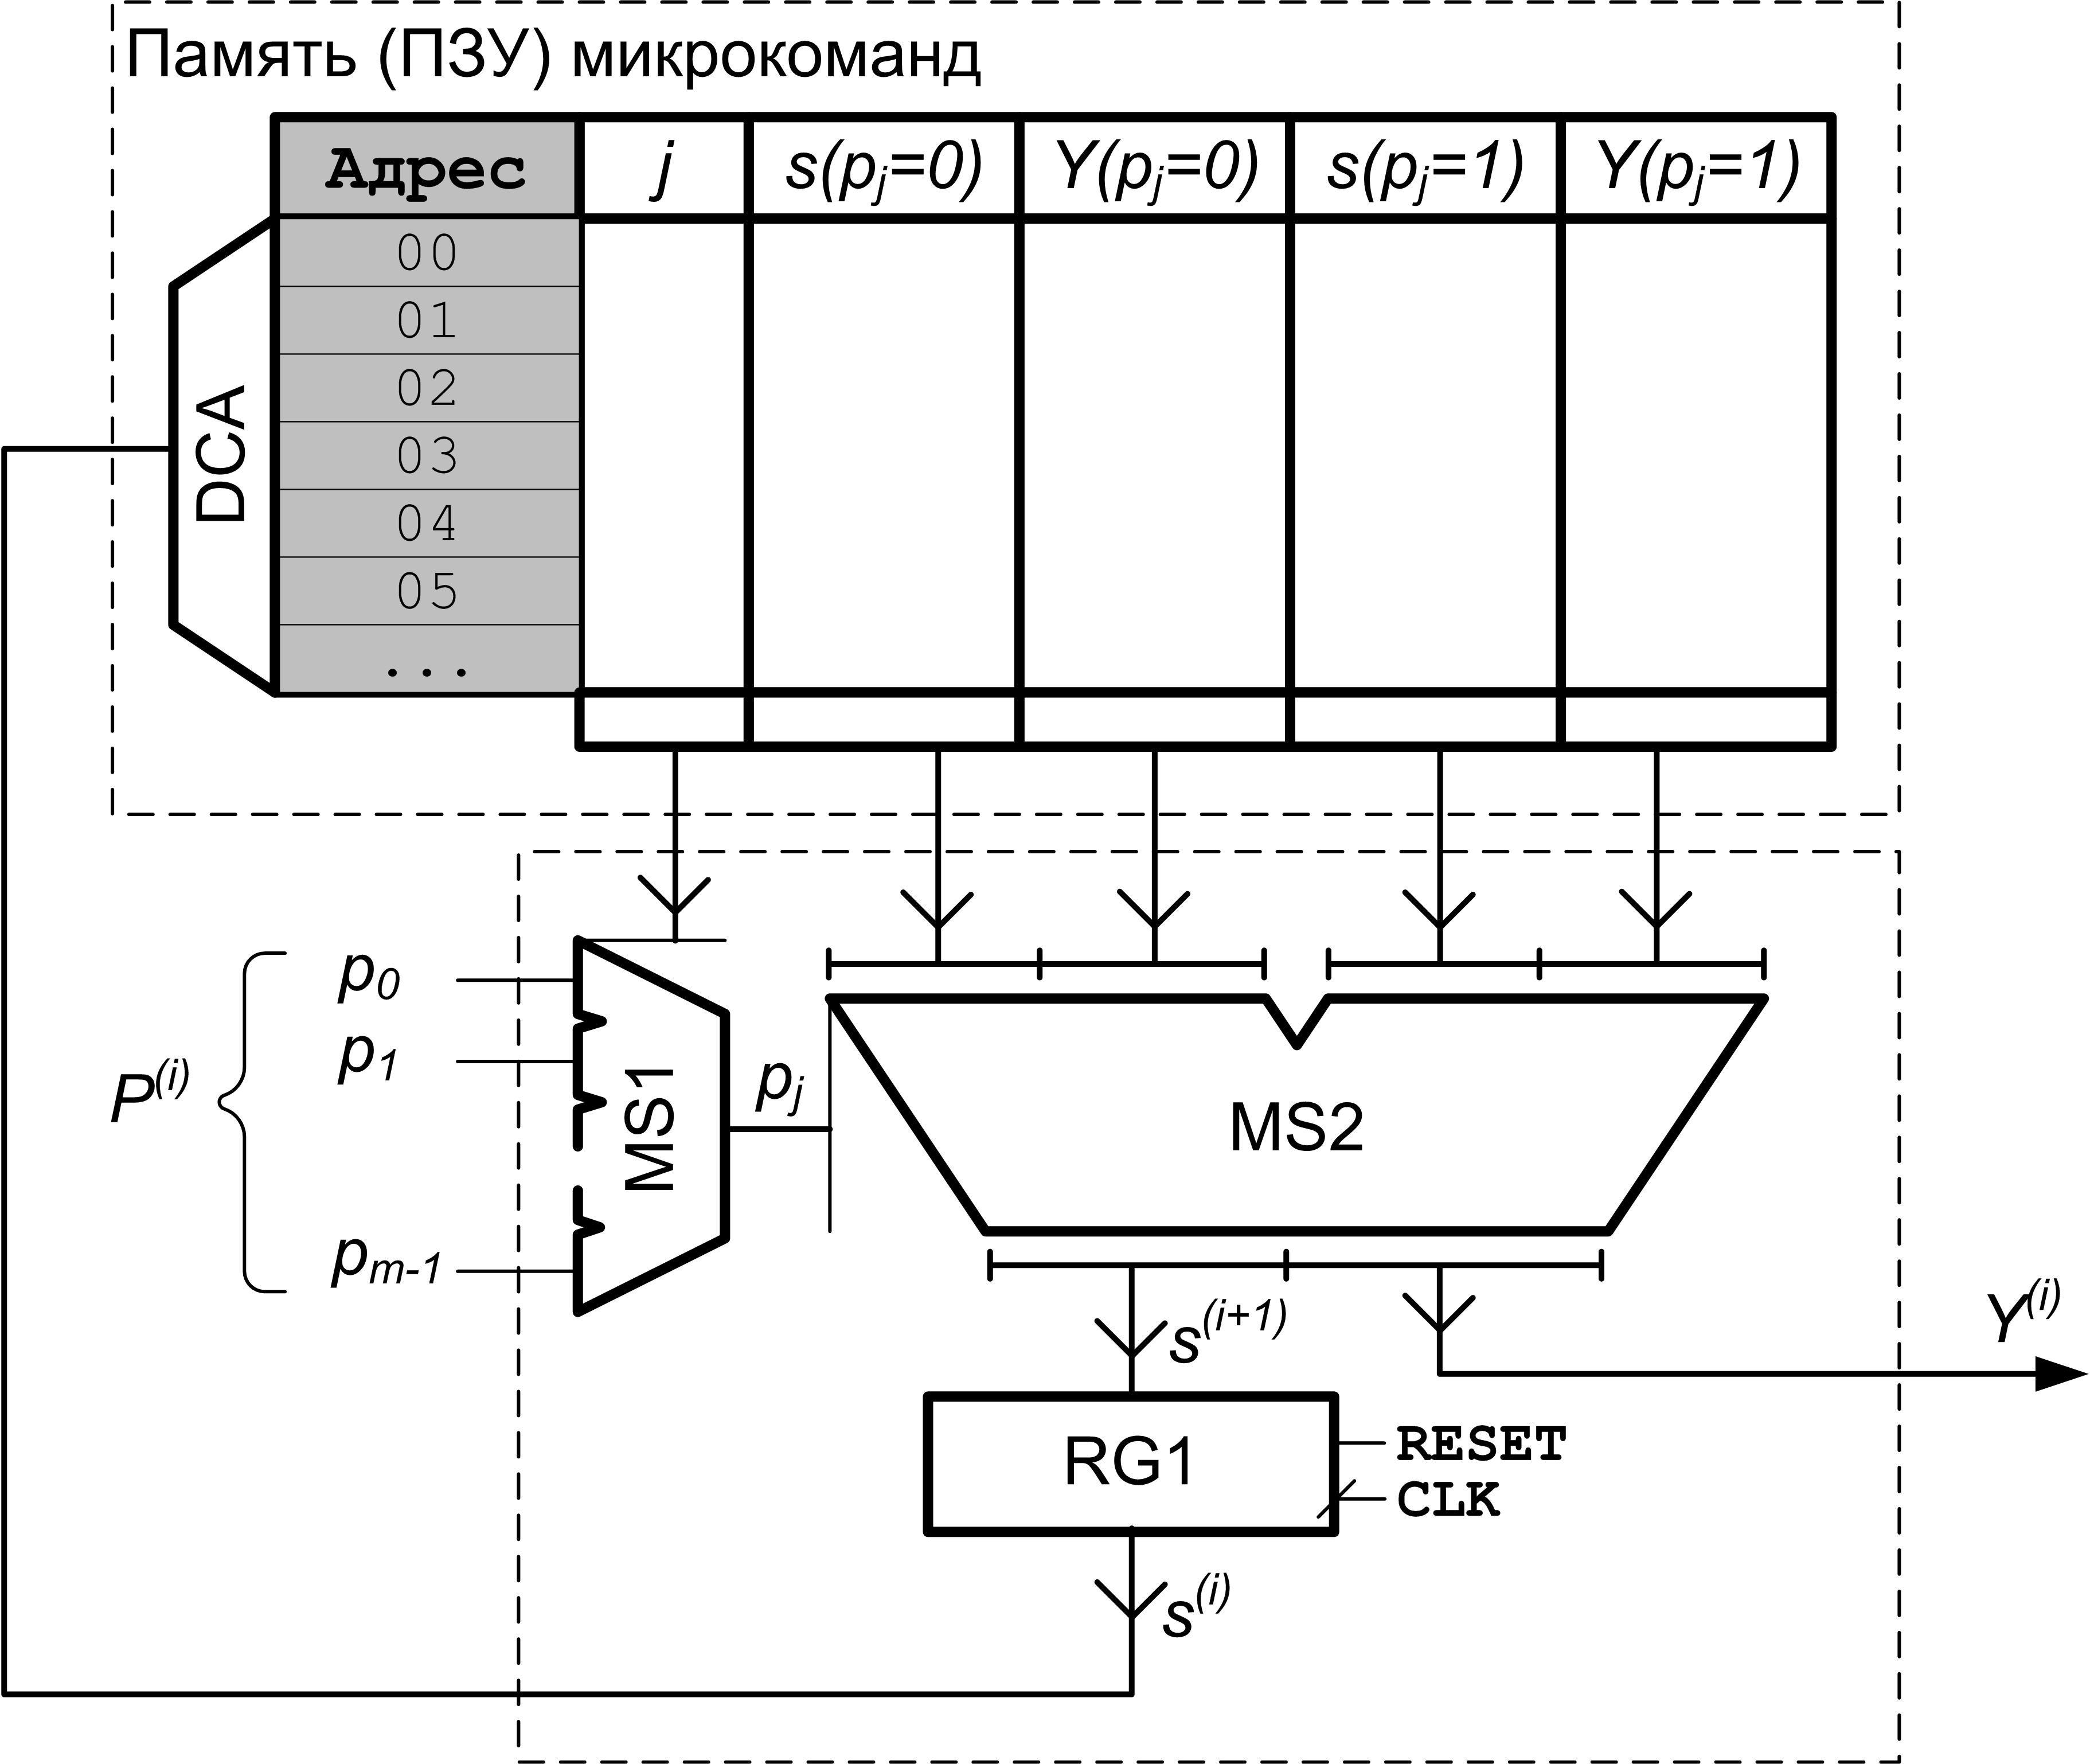
\includegraphics{fig/mili} 
    \caption{Автомат Мили}
    \label{fig::ch::practice::Mili}
\end{figure}

\begin{figure}[!ht]
    \centering
    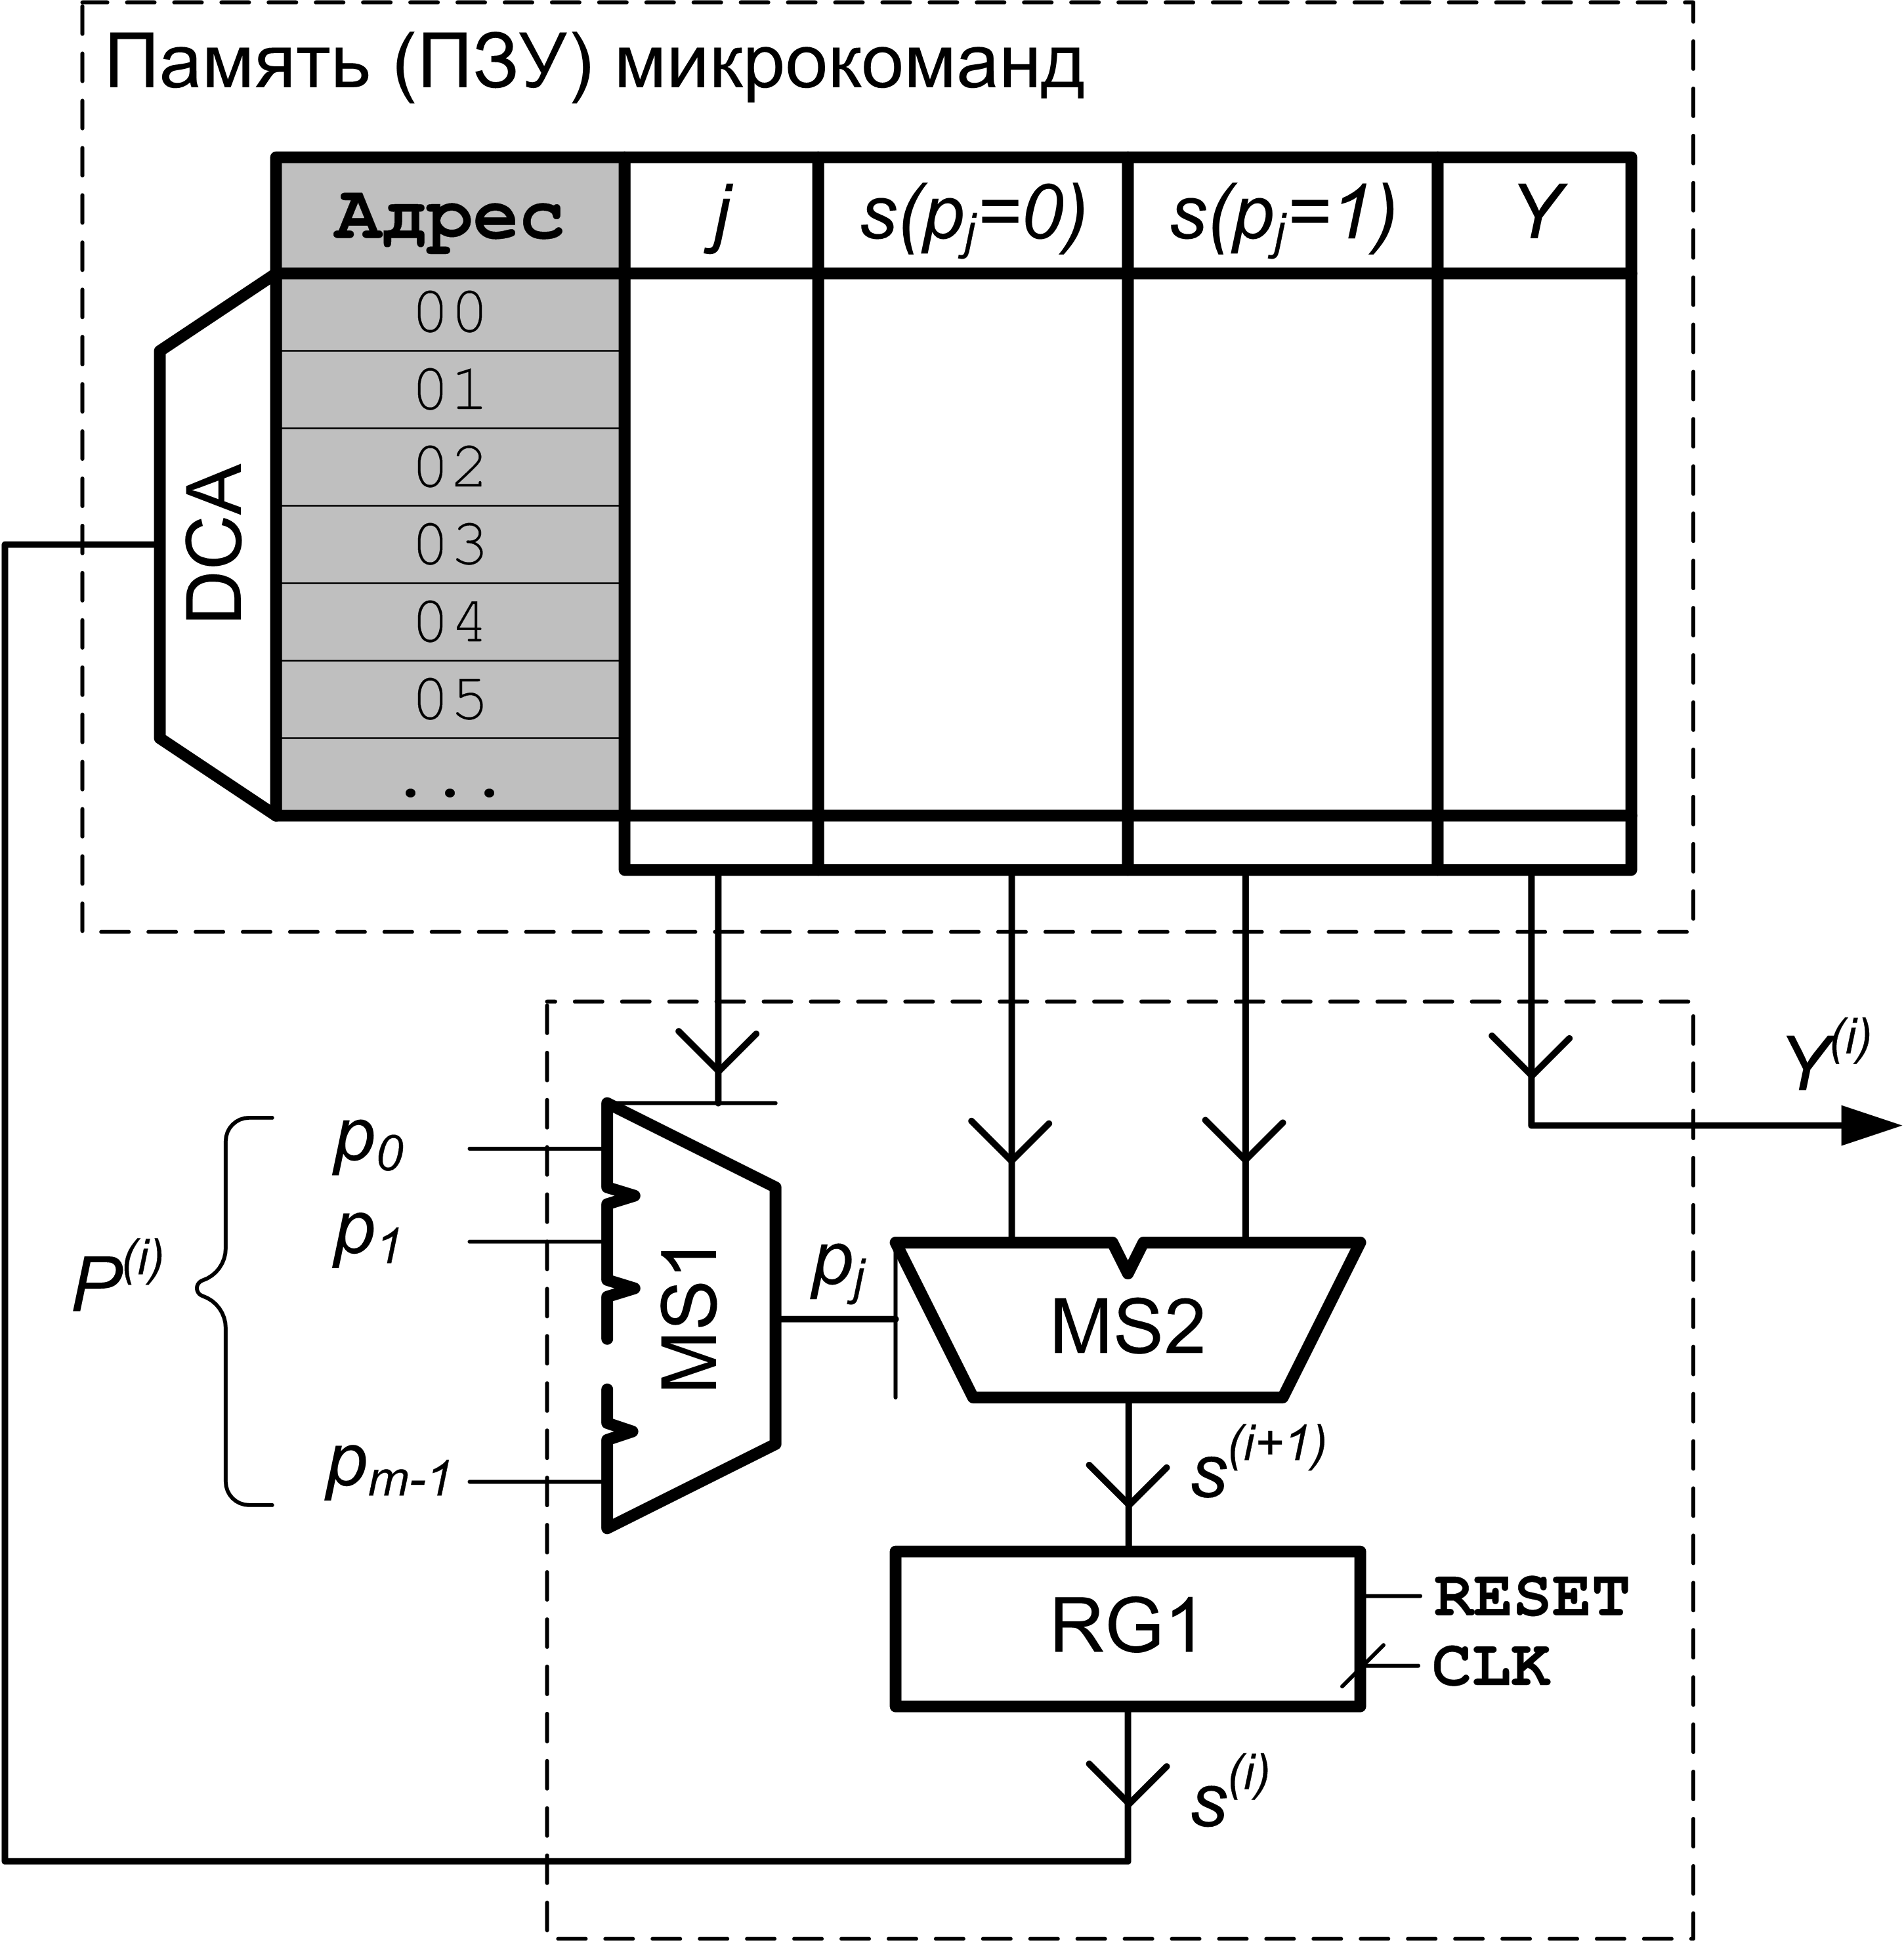
\includegraphics{fig/moore}
    \caption{Автомат Мура}
    \label{fig::ch::practice::Moore}
\end{figure}

В приведенных схемах микропрограммных автоматов выделены два блока --- <<Память (ПЗУ) микропрограмм>> и элементарное управляющее устройство. Текущему состоянию автомата $S^{(i)}$ соответствует адрес в памяти микропрограмм, то есть текущее состояние определяет адрес микрокоманды. Адрес (состояние) в течение такта снимается с выхода \Machine{RG1}. По завершению такта, в регистре \Machine{RG1} будет запомнено новое состояние, которое будет выдаваться в течение следующего такта. \Machine{RG1} переключается в каждом такте под управлением тактового сигнала \Machine{CLC}.

Ячейка памяти имеет для обоих автоматов общие части: 
\begin{itemize}
    \item поле $j$ --- выбор осведомительного сигнала (т.е. на управление \Machine{MS2} будет поступать значение осведомителного сигнала $p_j$);
    
    \item поле $S(p_j=0)$ --- новое состояние автомата, которое будет занесено в \Machine{RG1}, если $p_j=0$;
    
    \item поле $S(p_j=1)$ --- состояние, в которое перейдет автомат при $p_j=1$;    
\end{itemize}

Работа автомата начинается со сброса регистра \Machine{RG1} сигналом \texttt{RESET} в 0 --- автомат переходит в состояние $s_0$. 

Выход регистра \Machine{RG1} поступает на адресный вход памяти микрокоманд и через некоторое время значение ячейки памяти с указанным адресом поступает на выход модуля памяти. Значение поля $j$ управляет мультиплексором \Machine{MS1}, на выходе которого появляется значение осведомительного сигнала $p_j$, которое в свою очередь поступает на вход управления \Machine{MS2}. На выходе \Machine{MS2} появляется одно из двух состояний автомата: либо значение поля $S(p_j=0)$, либо --- поля $S(p_j=1)$. При переходе в следующий такт под управлением сигнала \Machine{CLC} регистр \Machine{RG1} запомнит новое состояние, сформировавшееся на выходе \Machine{MS2}.

В автомате Мили вектор управляющих сигналов снимается с выхода \Machine{MS2}, который осуществляет выбор из двух значений\footnote{
    На практике автомат Мили <<не прощает>> ошибок проектирования: когда значение сигнала $p_j$ меняется под воздействием управляющего сигнала в том же такте (такое бывает, когда значение $p_j$ снимается с выхода элемента логики, а не памяти, и соответсвенно может измениться в течение такта). Такое взаимовлияние может привести к <<гонкам>> осведомительных и управляющих сигналов и полной неопределенности в вопросе: <<в какое же из двух возможных состояний перейдет автомат Мили?>>
}, хранимых в памяти: $Y(p_j=0)$ и $Y(p_j=1)$;

В автомате Мура вектор управляющих сигналов определяется только текущим состоянием, поэтому снимается непосредственно с модуля памяти (поле $Y$).

В $i$-м такте работы управляющего устройства происходит следующее:
\begin{enumerate}
    \item Поступают осведомительные сигналы $P^{(i)}$. Эти осведомительные сигналы отражают изменения, произошедшие в предыдущем такте и в течение $i$-го такта не изменяются (так как снимаются обычно с выходов элементов памяти).
    
    \item Управляющее устройство формирует и выдает управляющие сигналы $i$-го такта. Также управляющее устройство определяет состояние $s^{(i+1)}$ в которое оно перейдет по завершении $i$-го такта. Значения управляющих сигналов стабилизируются, они распространяются по схеме и на сответствующих входях элементов памяти устанавливаются корректные значения.
    
    \item В конце такта (в зависимости от управляющих сигналов) в операционной части происходит защелкивание необходимых значений в элементах памяти. В частности, желательно сохранять в элементах памяти значения осведомительных сигналов.
\end{enumerate}

Одному такту работы схемы автомата Мили на рисунке \ref{fig::ch::practice::Mili} можно сопоставить фрагменты граф-схемы алгоритма, приведенные на рисунке \ref{fig::ch::practice::MiliAlg}. Состояния автомата выделены серыми кружками-пометками. Автомат Мили в том же такте реагирует (управляющими сигналами) на осведомительные сигналы.

\begin{figure}[!ht]
    \centering
    \begin{tabular}{c|c}
        \raisebox{-.5\height}{
            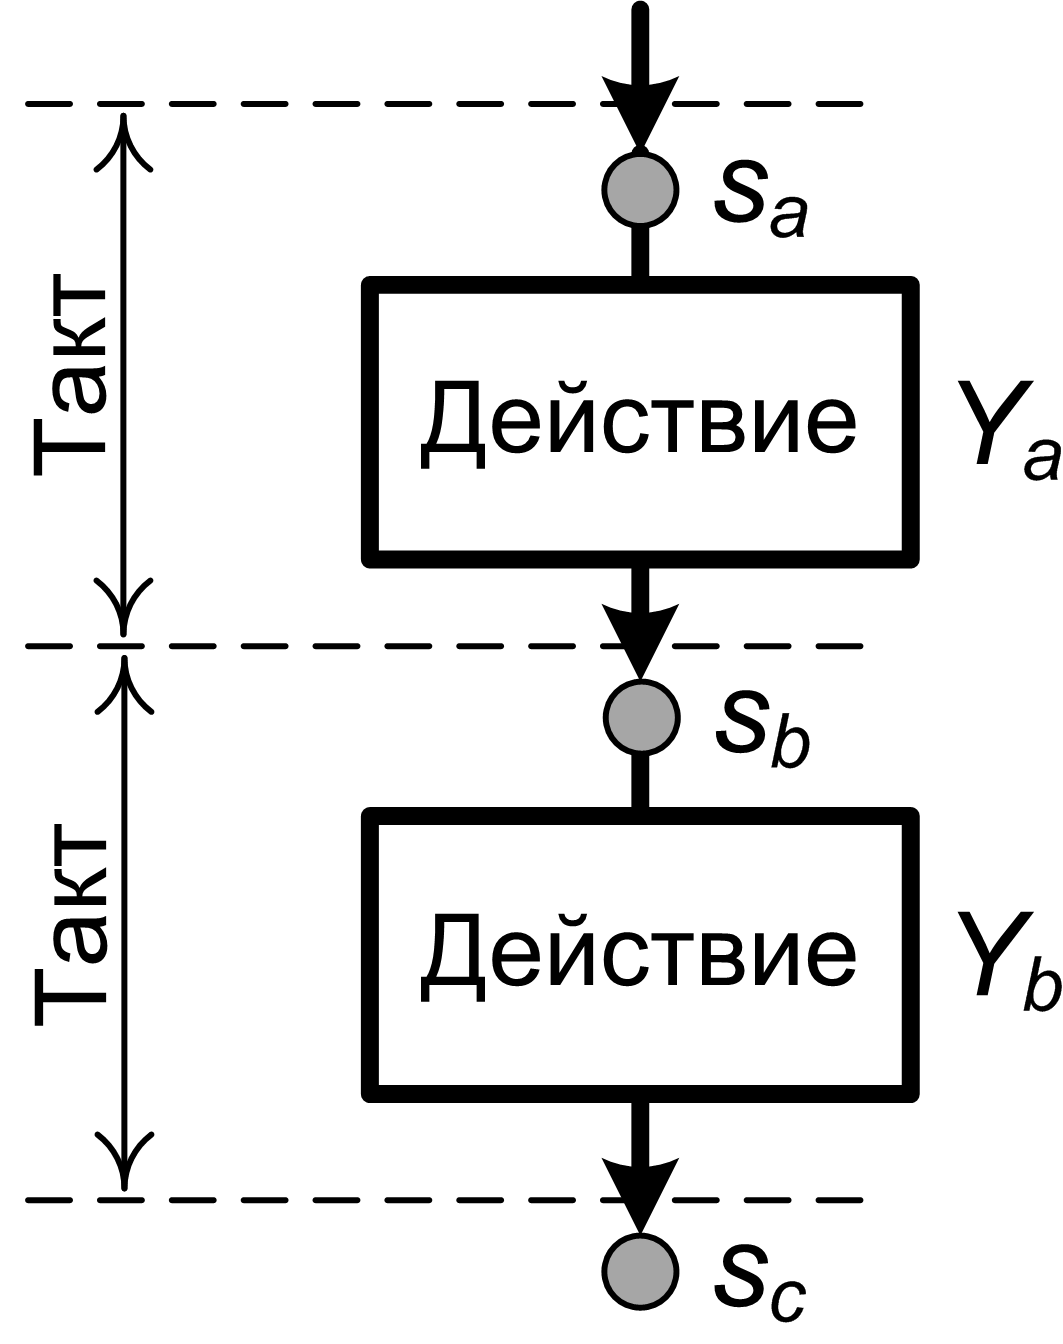
\includegraphics{fig/MiliAlgSeq}
        }
        &
			\raisebox{-.5\height}{
				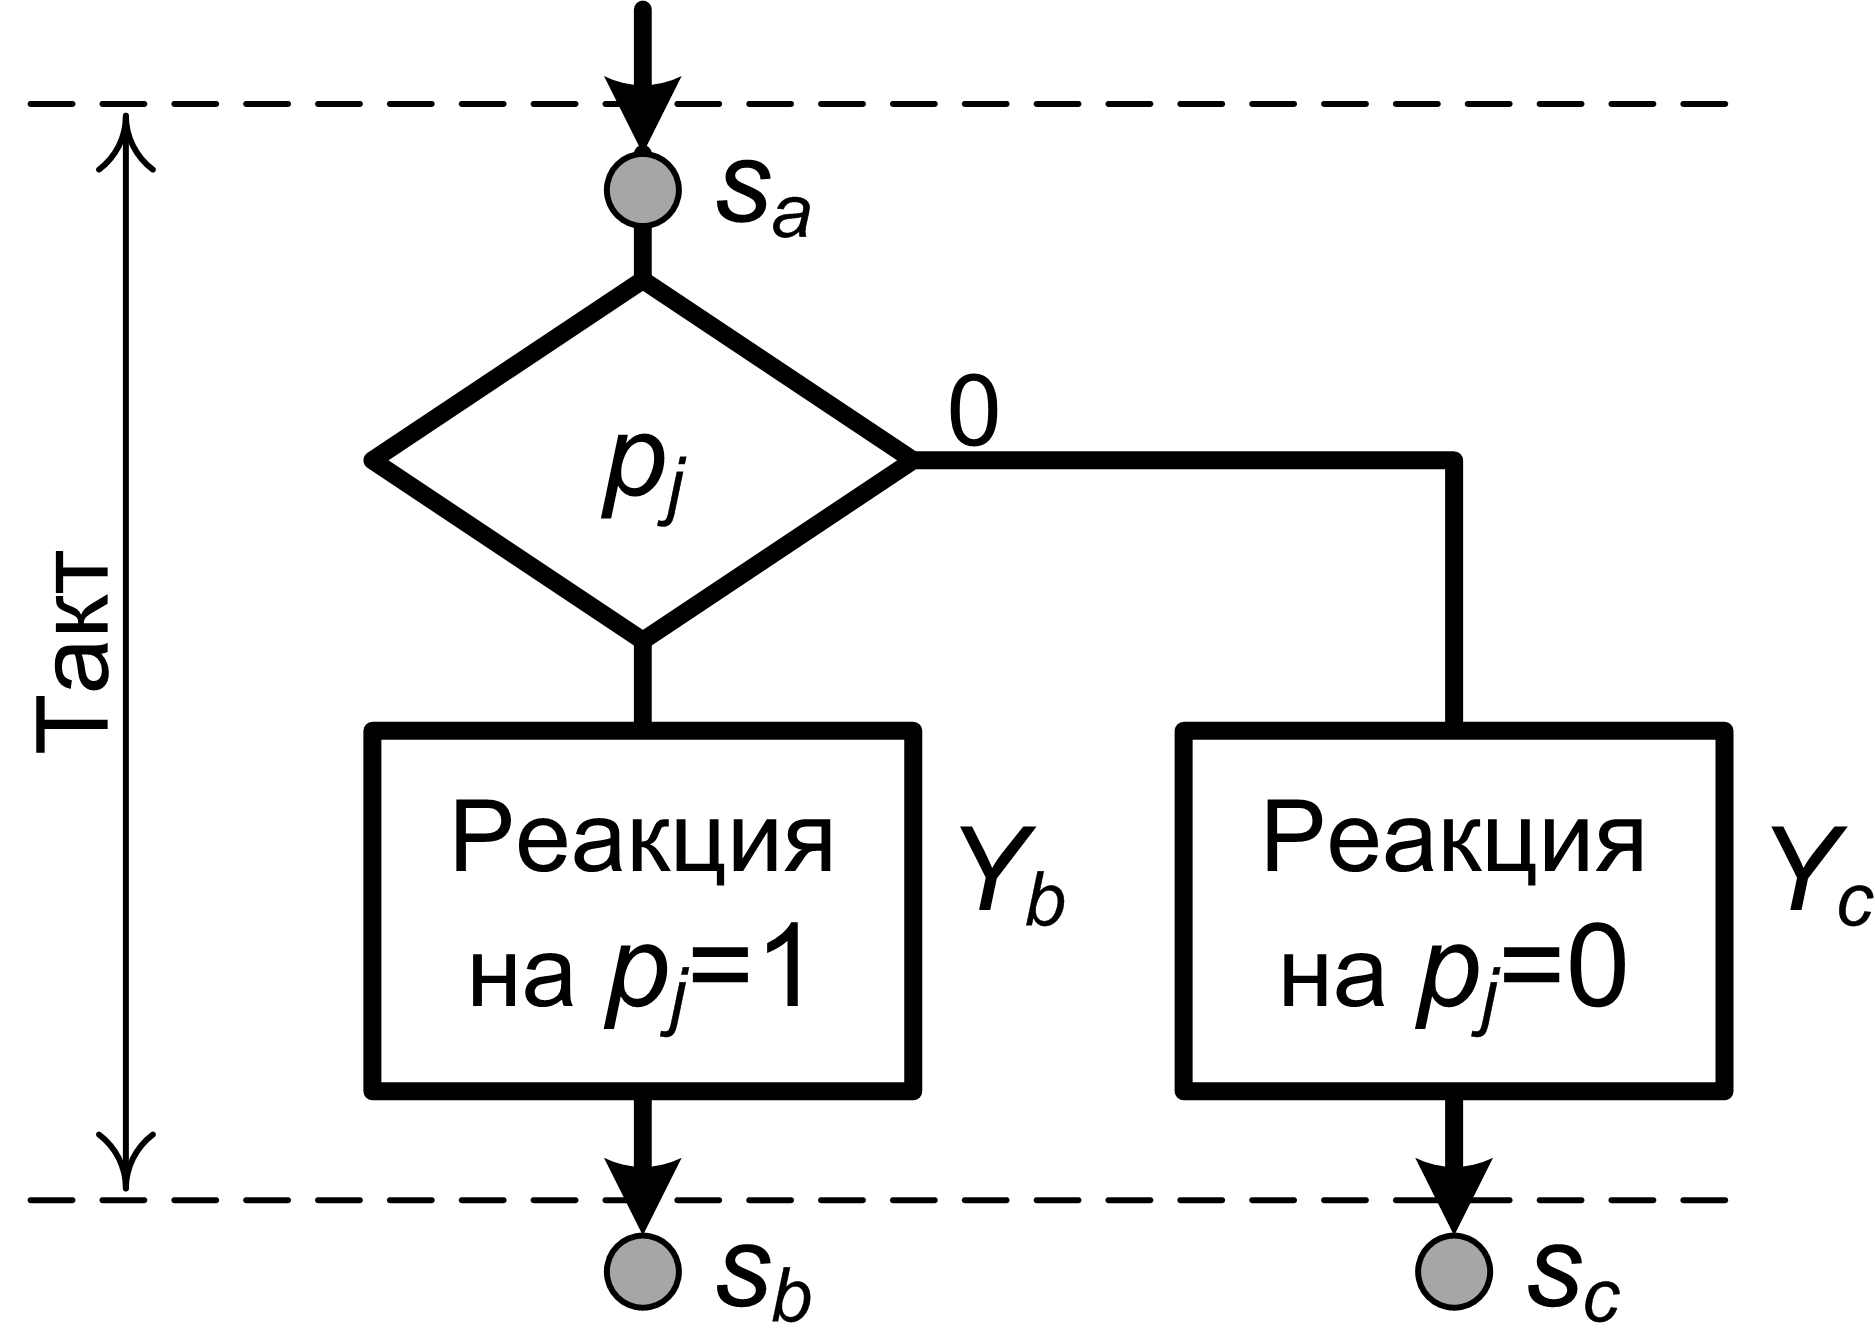
\includegraphics{fig/MiliAlgIf}
			} 
			\\
        {\xymatrix{
            S_a \ar@{->}[r]^{*|Y_a} 
                &S_b \ar@{->}[r]^{*|Y_b} 
					&S_c 
        }}
		&
			{\xymatrix{
				S_a \ar@{->}@/^/[r]^{\bar{p}_j|Y_c} 
					\ar@{->}@/_/[dr]_{p_j|Y_b} 
					&S_c \\
				*{} &S_b
			}}
			\\
    \end{tabular}
    \caption{Примеры фрагментов алгоритмов, реализуемых автоматом Мили за один такт}
    \label{fig::ch::practice::MiliAlg}
\end{figure}

Граф-схема, соответствующая такту работы автомата Мура (рис. \ref{fig::ch::practice::Moore}) приведена на рисунке \ref{fig::ch::practice::MooreAlg}. Автомат Мура реагирует на осведомительные сигналы только в следующем такте. 

\begin{figure}[!ht]
    \centering
    \begin{tabular}{c|c}
        \raisebox{-.5\height}{
            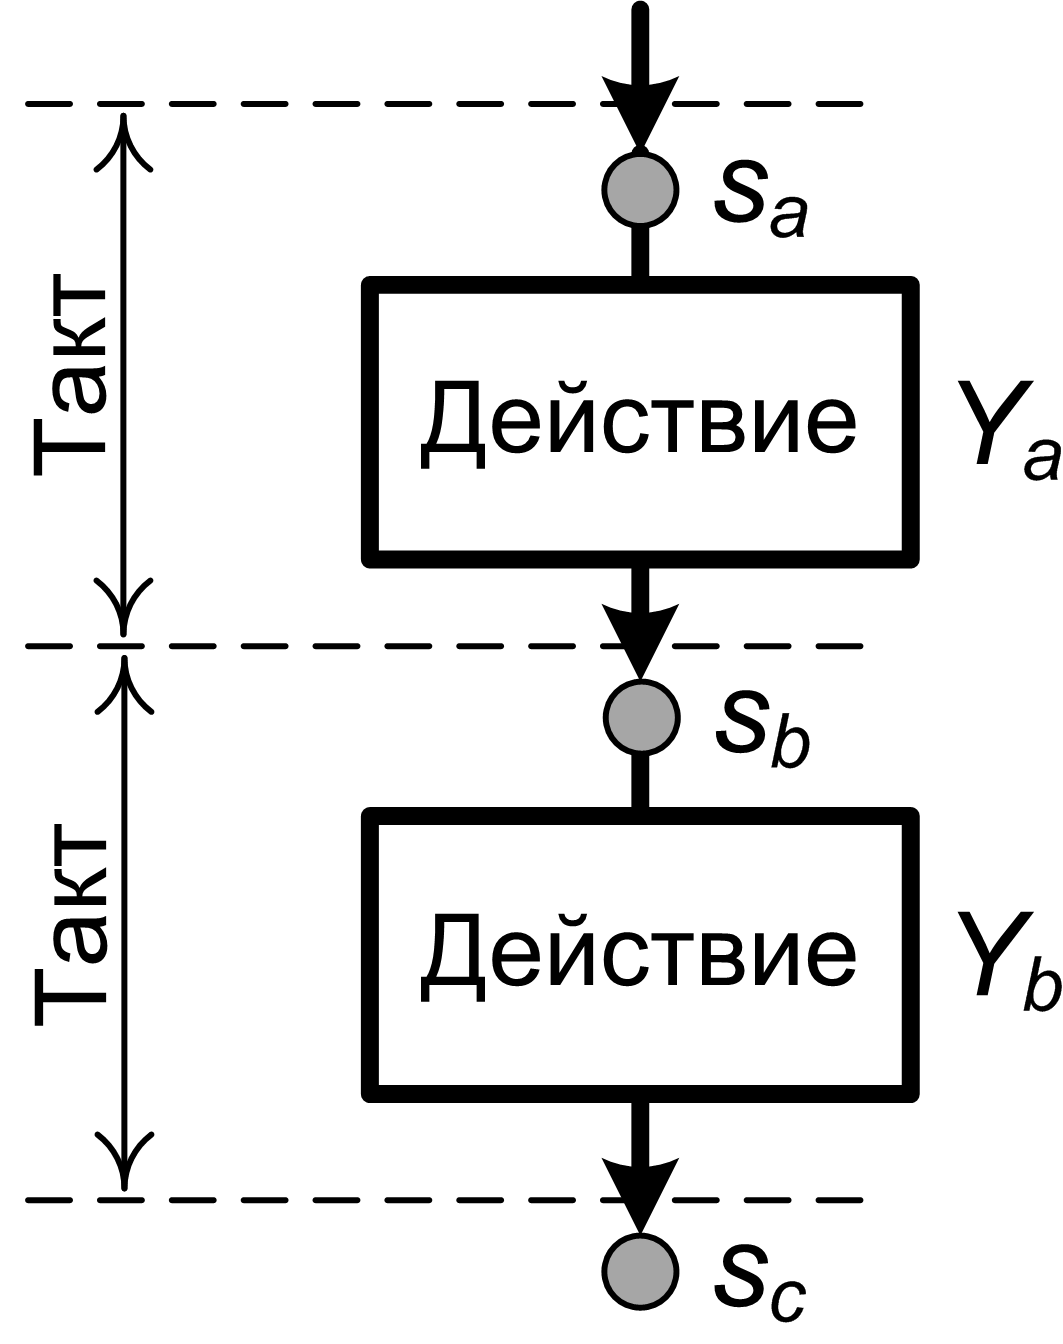
\includegraphics{fig/MooreAlgSeq}
        }
        &
			\raisebox{-.5\height}{
                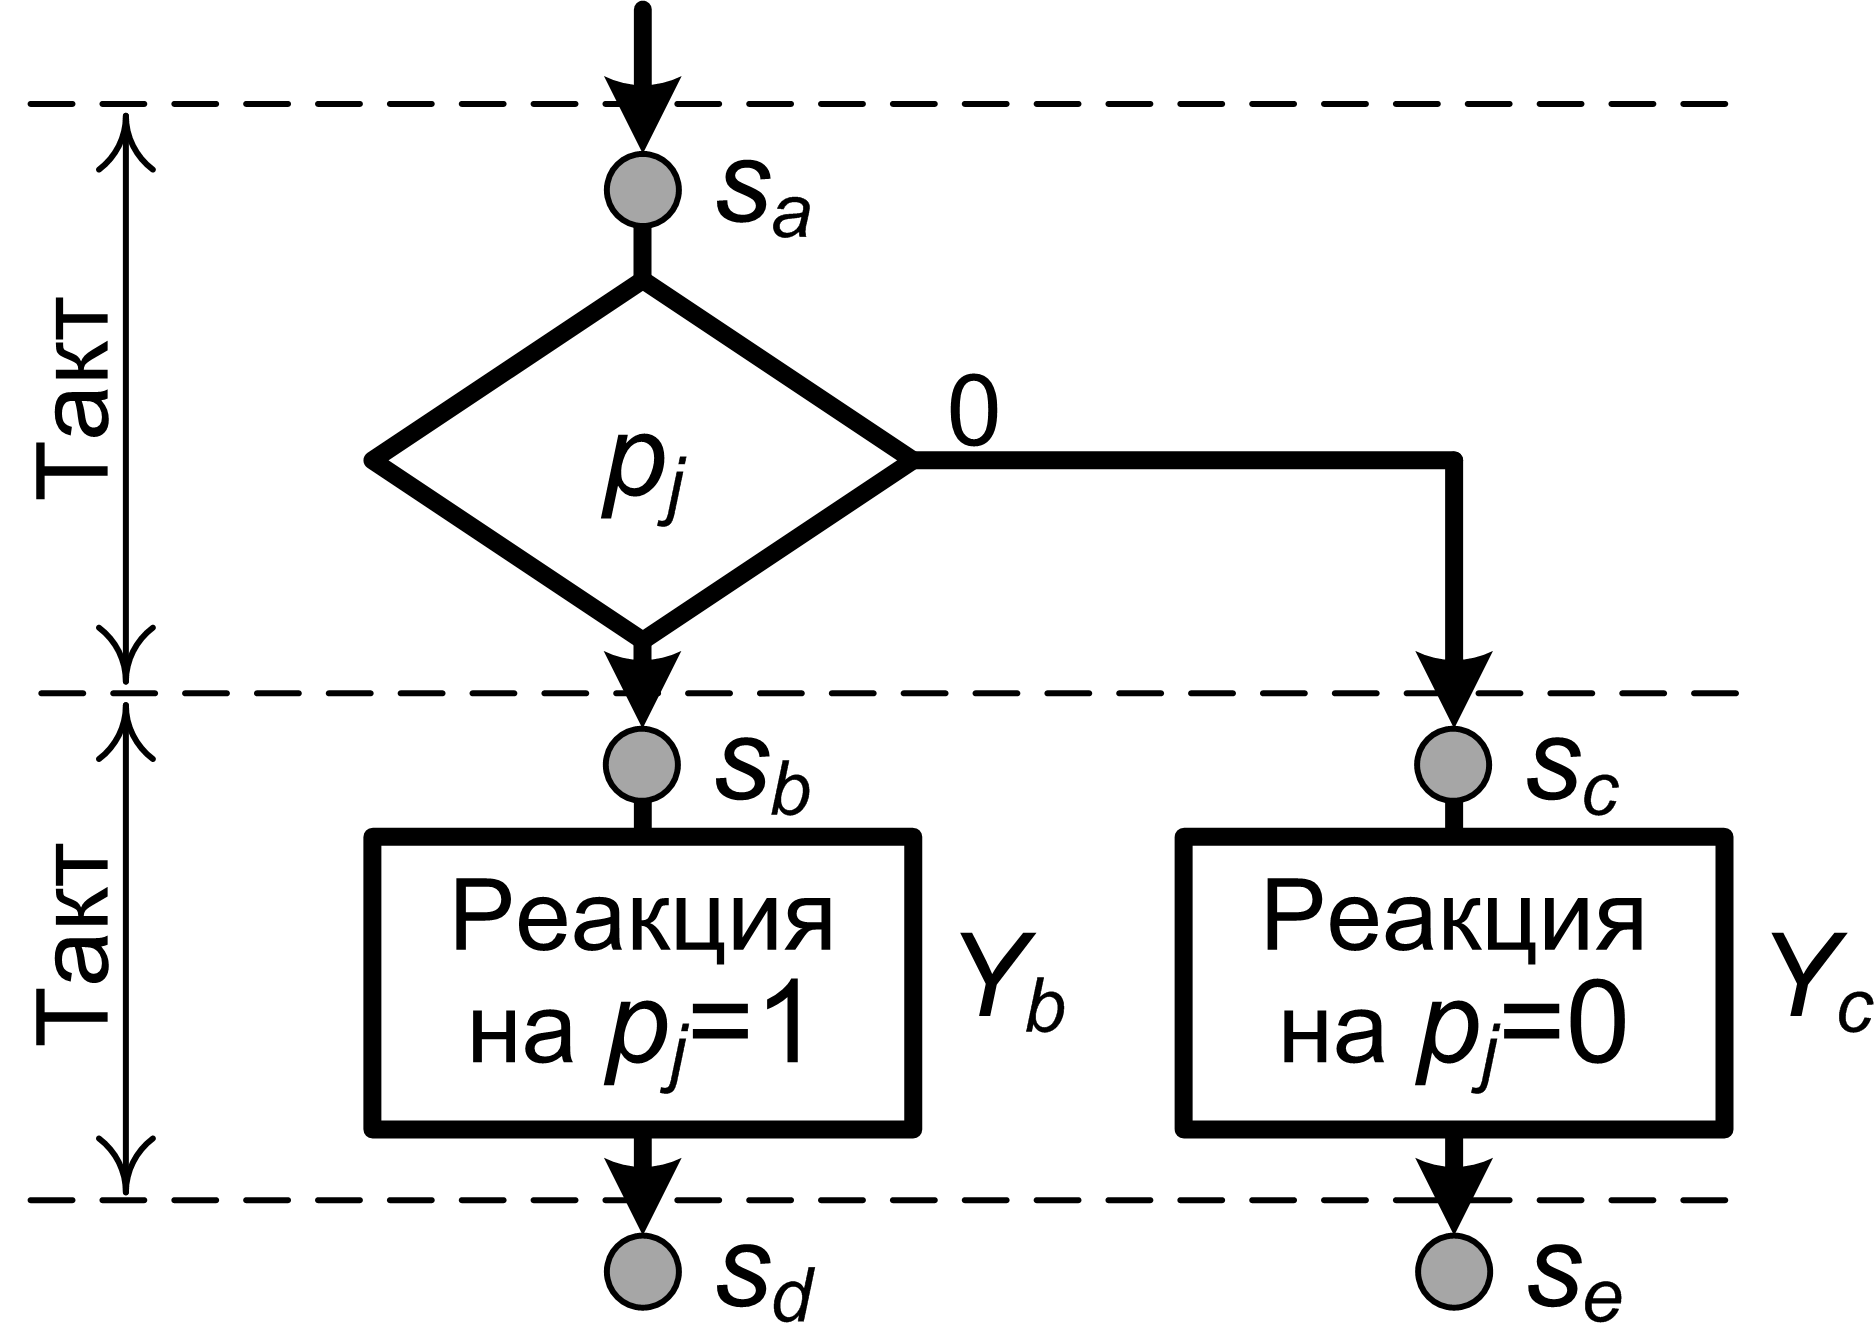
\includegraphics{fig/MooreAlgIf}
            }
			\\
        {\xymatrix{
            S_a|Y_a \ar@{->}[r]^{*} 
                &S_b|Y_b \ar@{->}[r]^{*} 
                    &S_c| \\
        }}
        &
            {\xymatrix{
                S_a|\Machine{0h} \ar@{->}@/^/[r]^{\bar{p}_j} 
                    \ar@{->}@/_/[dr]_{p_j} 
                    &S_c|Y_c \ar@{->}[r]^{*} 
                        &S_e|
                        \\
                *{} 
                    &S_b|Y_b \ar@{->}[r]^{*} 
                        &S_d|
            }}            
    \end{tabular}
    \caption{Примеры фрагментов алгоритма, реализуемых автоматом Мура за один такт}
    \label{fig::ch::practice::MooreAlg}
\end{figure}

Видно, что автомат Мура тратит отдельный такт на анализ осведомительного сигнала, при этом в таком такте, конечно могут выдаваться и управляющие сигналы (в приведенном примере на Рис. \ref{fig::ch::practice::MooreAlg} выдается \Machine{0h}). То есть, можно совместить вершину процесса и условную вершину в одном состоянии, если процесс на условие не влияет и тогда процесс и анализ условия \emph{совмещаются} во времени. В противном случае, если имелось в виду, что \emph{после} определенных действий, следует проанализировать осведомительный сигнал, то следует выделить два состояния (см. пример на рисунке \ref{fig::ch::practice::MooreAlgFictive}).
\begin{figure}[!ht]
    \centering
    \begin{tabular}{c|c}
        \raisebox{-.5\height}{
            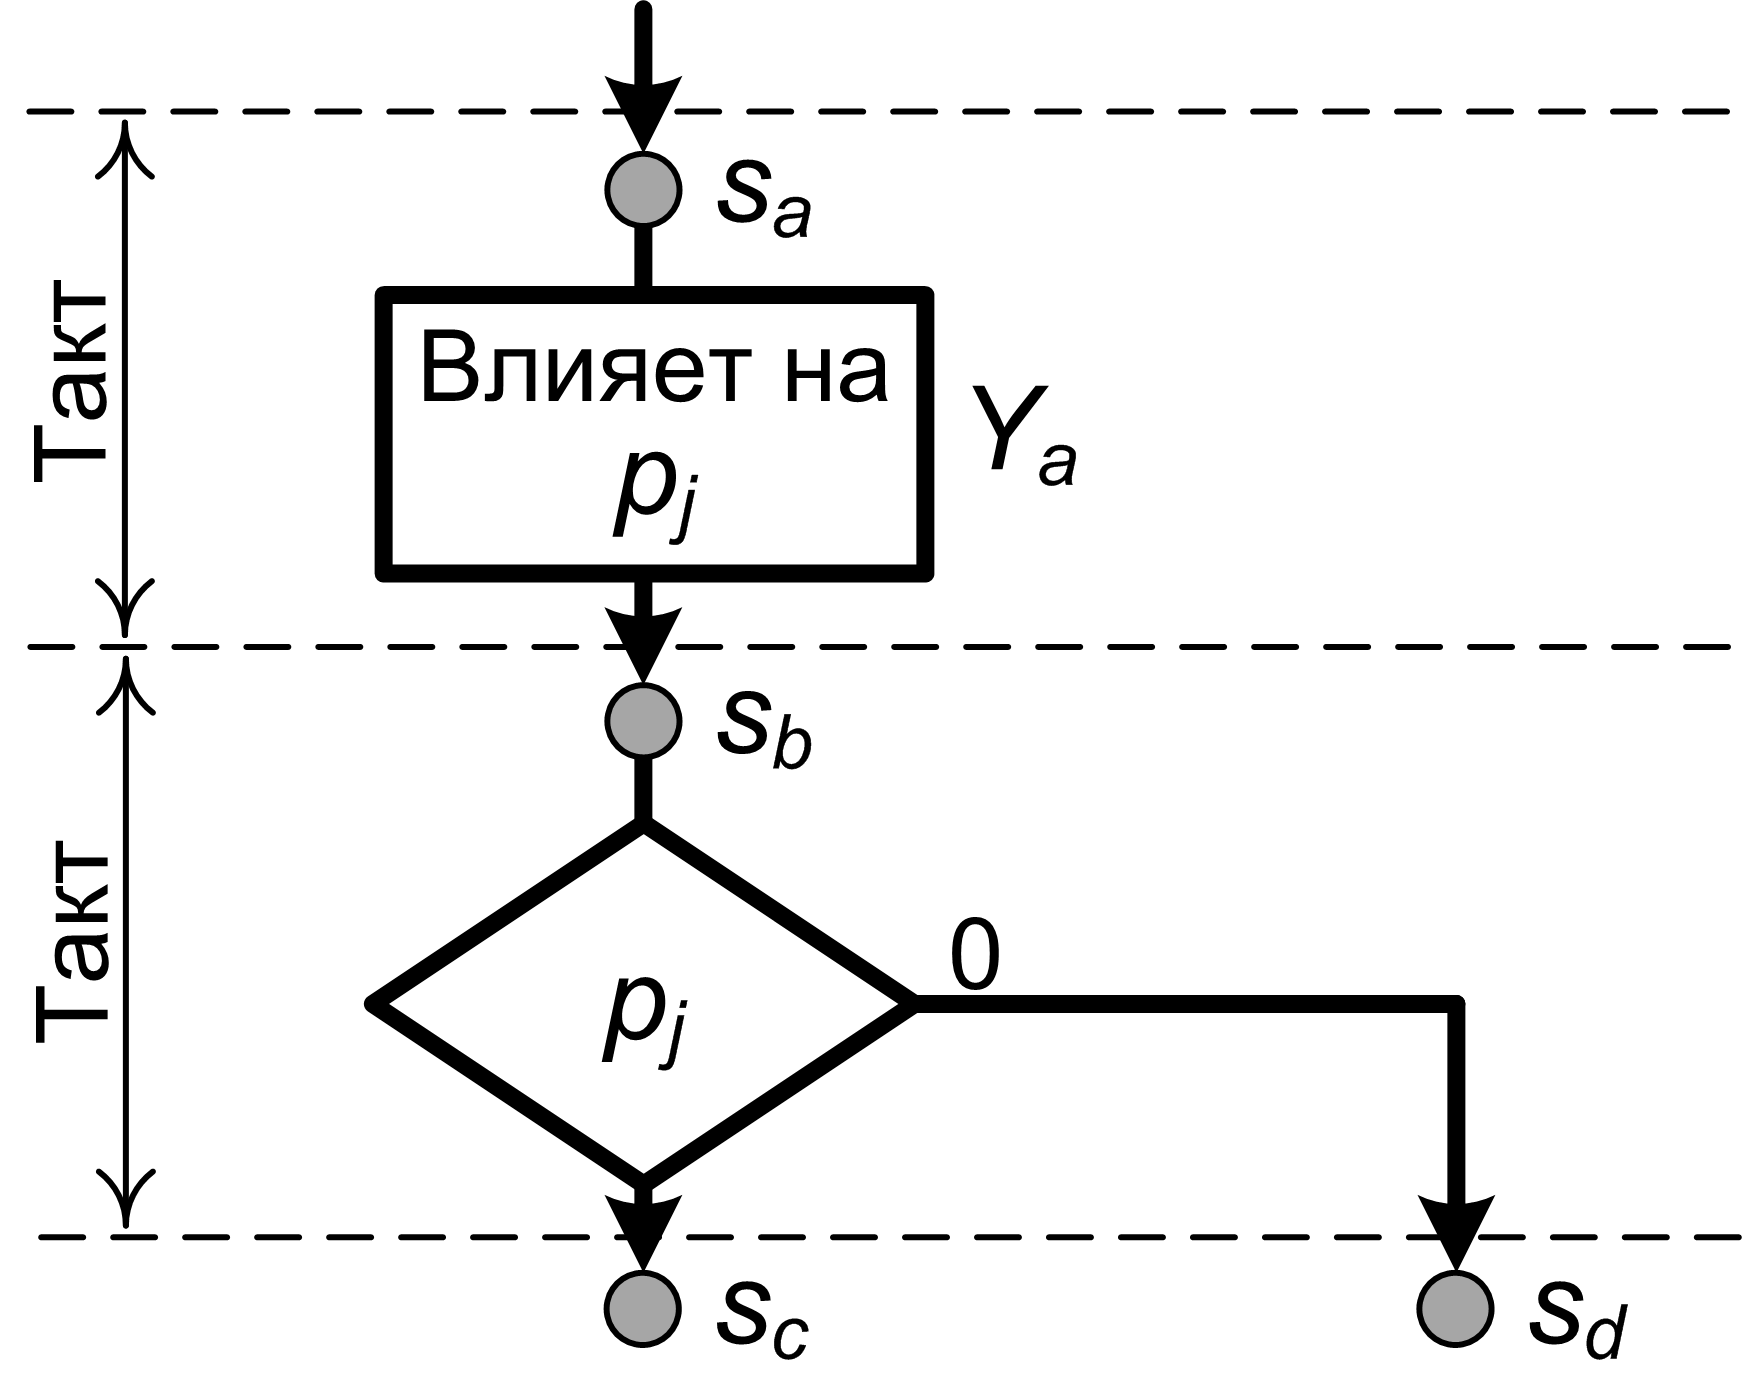
\includegraphics{fig/MooreIfTwo}
        }
        &
			\raisebox{-.5\height}{
                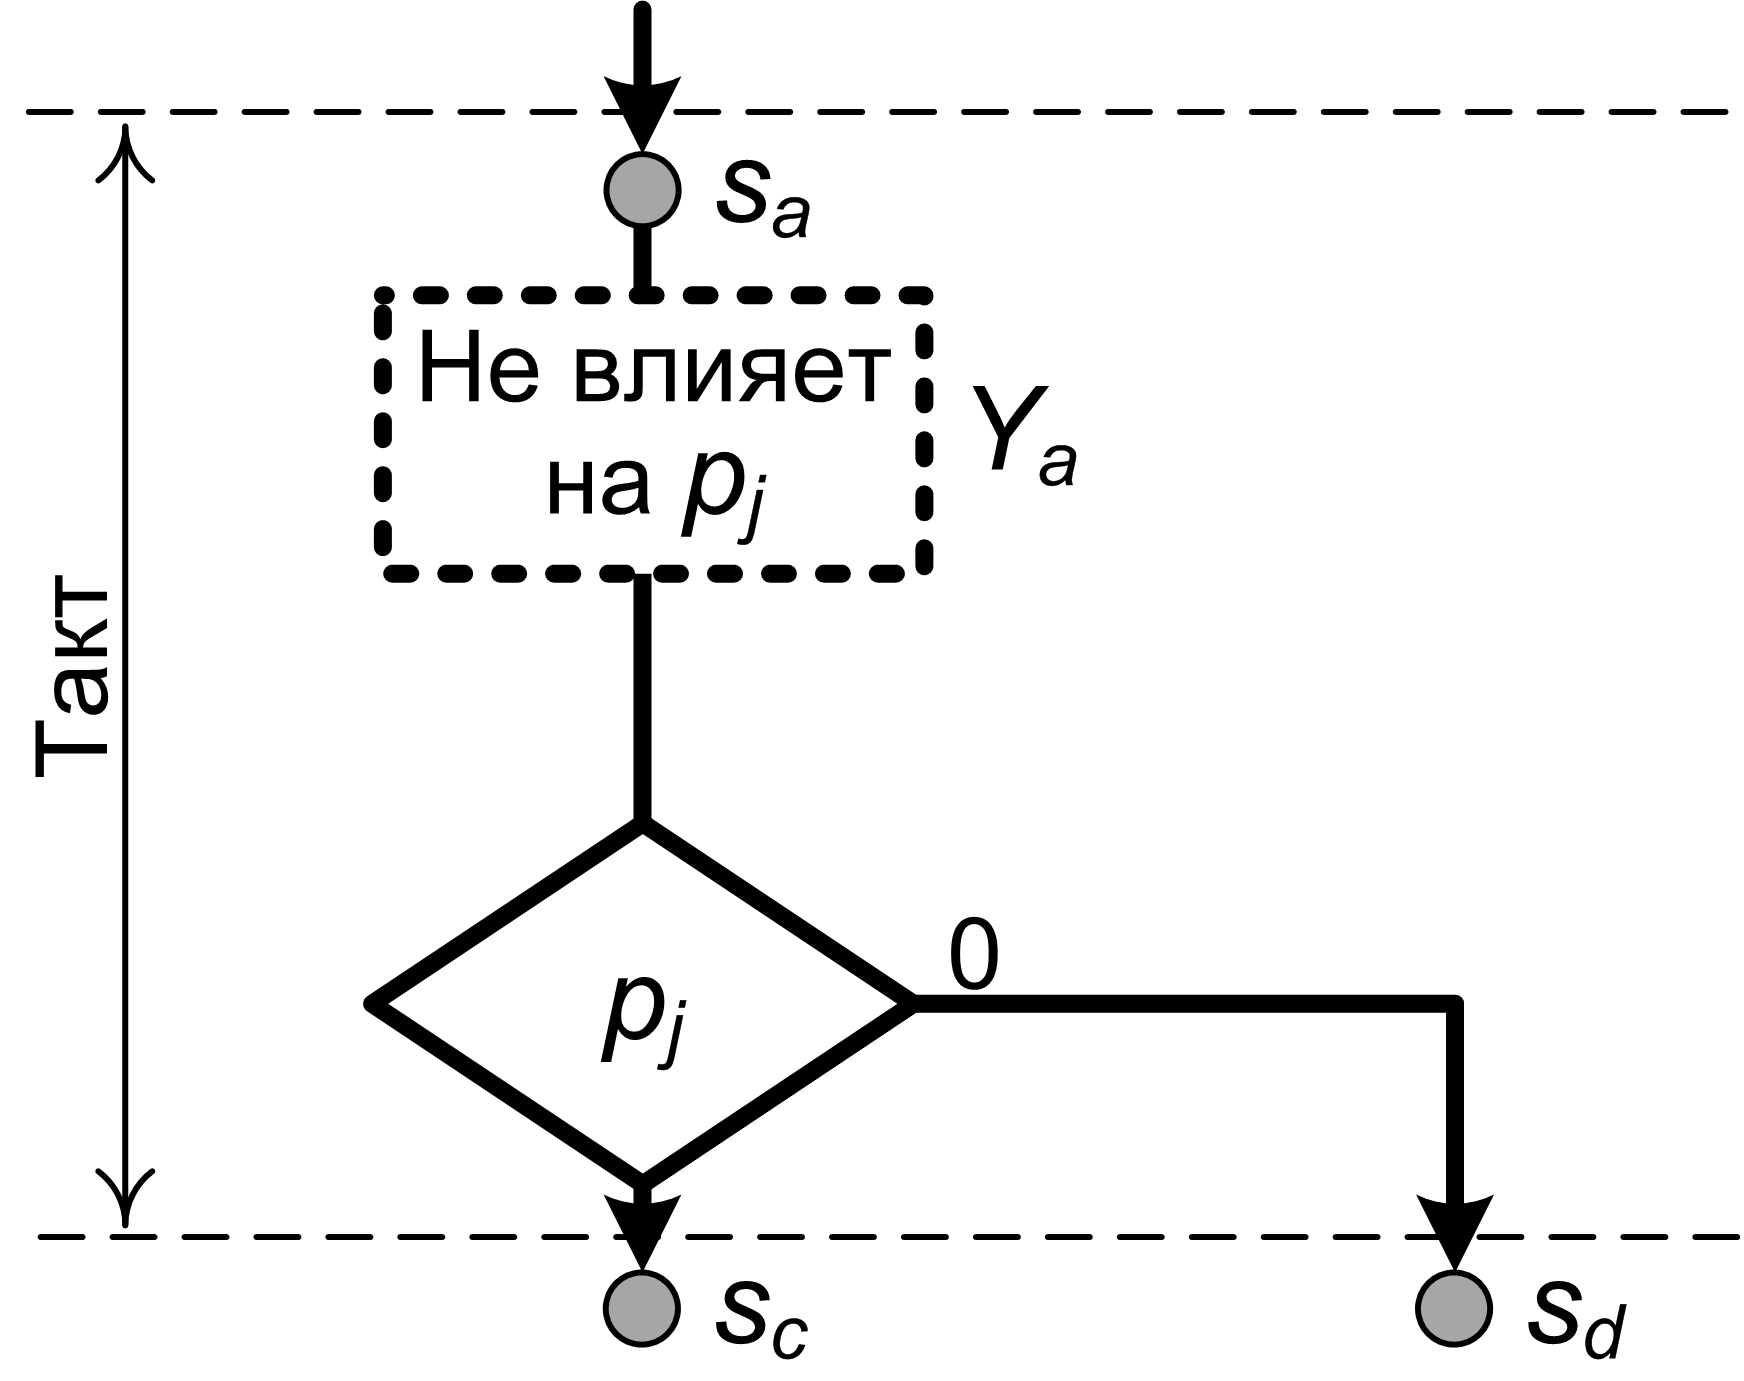
\includegraphics{fig/MooreIfOne}
            }
			\\
        {\xymatrix{
            S_a|Y_a \ar@{->}[r]_{*} 
                &S_b|\Machine{0h} \ar@{->}@/^/[r]^{\bar{p}_j}  
                                  \ar@{->}@/_/[dr]_{p_j} 
                    &S_d|
                    \\
            *{} 
                &*{}
                    &S_c|
        }}            
        &
            {\xymatrix{
                S_a|Y_a \ar@{->}@/^/[r]^{\bar{p}_j}  
                                      \ar@{->}@/_/[dr]_{p_j} 
                    &S_d|
                    \\
                *{}
                    &S_c|
        }}            
    \end{tabular}
    \caption{Особенности выделения состояний автомата Мура}
    \label{fig::ch::practice::MooreAlgFictive}
\end{figure}


На указанные фрагменты можно разбить любую произвольную схему алгоритма. Также при составлении алгоритма следует учитывать указанные особенности автомата, выполняющего этот алгоритм. Детальное обсуждение особенностей находится за рамками данного курса, поэтому далее рассматривается пример микропрограммирования, который позволить понять суть микропрограммного управления.

\subsection{Соглашения о взаимодействии с ЦУУ}

Особенности взамодействия ОЧ множительного устройства и ЦУУ были изложены в самом начале раздела \ref{ch::practice}. Введем следующие обозначения сигналов:
\begin{itemize}
    \item $p_0\Machine{(TASK)}$ --- <<Задание на шине>> от ЦУУ;
    \item $p_1\Machine{(BUS)}$ --- <<Шина твоя>> от ЦУУ;
    \item $y_0\Machine{(READY)}$ --- <<Свободен>> в ЦУУ;
    \item $y_1\Machine{(RESULT)}$ --- <<Результат готов>> в ЦУУ;
    \item \Machine{CLK} --- тактовые импульсы, синхронизирующие все устройства вычислительной системы в целом;
    \item \Machine{X(DATA)} --- данные на шине данных, могут выдаваться как ЦУУ (исходные операнды), так и множительным устройством (результат).
\end{itemize}

Изменение сигналов принято изображать на временной диаграмме. Высокий уровень сигнала на диаграмме соответствует логической единице, низкий --- нулю.

\begin{figure}[!ht]
    \centering
    \includegraphics{fig/timings.1}
    \caption{Временная диаграмма получения задания}
    \label{fig::ch::practice::timingsTr}
\end{figure}

Состояние шины (жгута) изображается по особому: так как на диаграмме обычно нет места, чтобы изобразить все линии шины по отдельности, то состояние шины изображают как один сигнал (см. сигнал \Machine{X(DATA)}). Когда состояние шины не имеет значения (на рисунке \ref{fig::ch::practice::timingsTr} это такты 0 и 3), то рисуют линию посередине между высоким и низким уровнем. При этом по шине могут передаваться данные для других устройств.

Когда на шину поступают данные, которые важны, их изображают двумя линиями, проведенными на высоком и низком уровнях одновременно (такты 1, 2 на рисунке \ref{fig::ch::practice::timingsTr}), а если нужно указать значение двоичного вектора на шине, то между линиями пишут соответствующее шестнадцатиричное значение.

На рисунке \ref{fig::ch::practice::timingsTr} изображена временная диаграмма получения задания от ЦУУ. Устройства следуют следующим соглашениям.
\begin{enumerate}
    \item УЧ выдает в ЦУУ сигнал $y_0\Machine{(READY)}$. См. такт 1. Таким образом УЧ сообщает ЦУУ, что множительное устройство готово решать новую задачу. Сигнал будет удерживаться до тех пор, пока ЦУУ не даст задание. 
    
    \item Когда ЦУУ потребуется выполнить умножение, то оно, убедившись, что множительное устройство готово ($y_0=1$), выдает в УЧ сигнал $p_0\Machine{(TASK)}$. См. такт 3. В последующих тактах ЦУУ будет выдавать фрагменты задания $\Machine{D}_1,\ldots,\Machine{D}_n$. В общем случае, задание состоит из одного фрагмента.
    
    ЦУУ выдает сигнал $p_0\Machine{(TASK)}$ только в течение одного такта.
    
    \item УЧ \emph{должна} в следующем такте, после получения сигнала  $p_0\Machine{(TASK)}$ от ЦУУ снять сигнал $y_0\Machine{(READY)}$ и начать чтение с шины первого фрагмента задания. См. такт 4. Пока УЧ решает задачу, сигнал $y_0\Machine{(READY)}$ не должен выдаваться.
\end{enumerate}

На рисунке \ref{fig::ch::practice::timingsRr} изображена временная диаграмма выдачи результата в ЦУУ. 

\begin{figure}[!ht]
    \centering
    \includegraphics{fig/timings.2}
    \caption{Временная диаграмма выдачи результата}
    \label{fig::ch::practice::timingsRr}
\end{figure}

\begin{enumerate} 
    \item УЧ выдает в ЦУУ сигнал $y_1\Machine{(RESULT)}$. См. такт 1. УЧ будет ждать момента, когда ЦУУ освободит шину и будет удерживать этот сигнал, пока не получит разрешение на передачу. См. такты 1-3. Количество тактов, в течение которых ЦУУ освобождает шину, варьируется, и непоправимой ошибкой будет выдача результата на <<занятую>> шину.

    \item ЦУУ, убедившись, что результат готов, выдает в течение одного такта сигнал $p_1\Machine{(BUS)}$. См. такт 3.
    
    \item УЧ, приняв сигнал $p_1\Machine{(BUS)}$ в следующем такте \emph{должно} снять сигнал $y_1\Machine{(RESULT)}$ и начать выдавать первый фрагмент результата. См. такт 4.
    
    \item УЧ как можно раньше должно выдать в ЦУУ сигнал $y_0\Machine{(READY)}$. Обычно, сигнал $y_0\Machine{(READY)}$ выдается в том же такте, в котором выдается последний фрагмент результата. См. такт $(n+3)$.
\end{enumerate}


\subsection{Пример микропрограммирования}
\label{ss::ch::practice::software::example}

В качестве примера рассматривается задача получения дополнительного кода из прямого. Несомненно, эту задачу можно решить проще.

Операционная часть устройства приведена на рисунке \ref{fig::ch::practice::dcconverter}.

\begin{figure}[!ht]
    \centering
    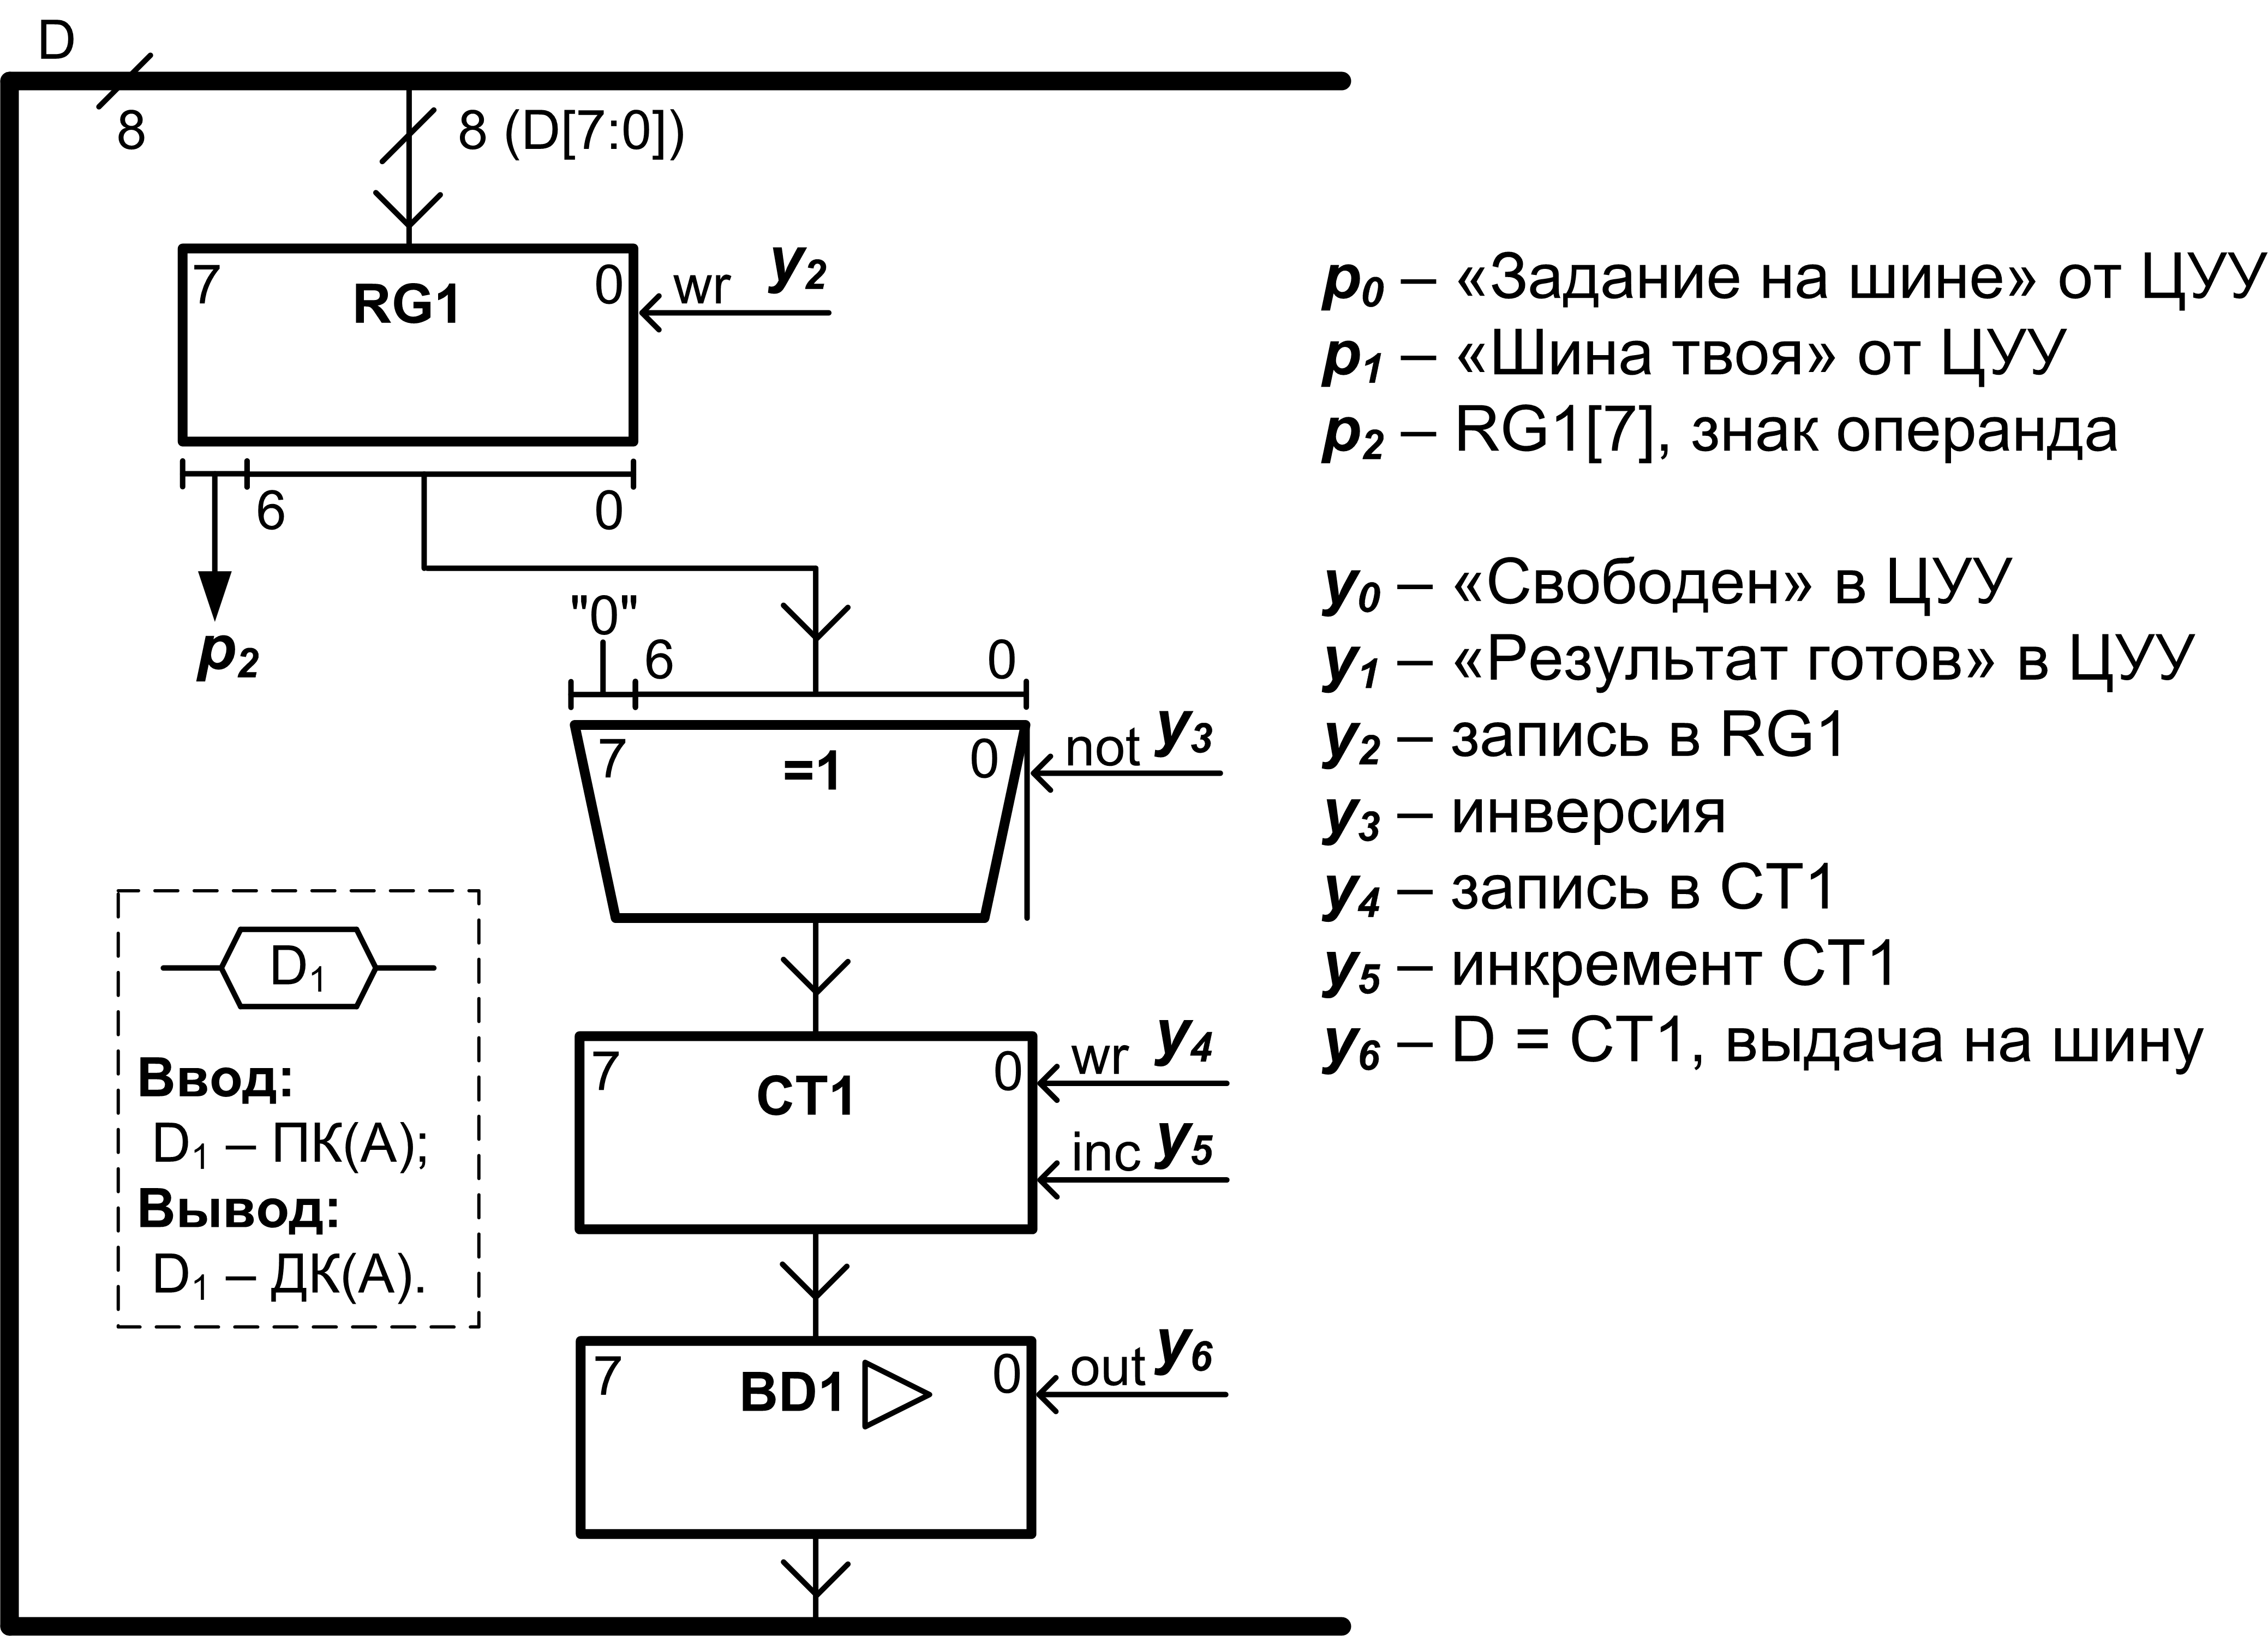
\includegraphics{fig/dcconverter}
    \caption{Операционная часть преобразователя $\Machine{ПК}\mapsto\Machine{ДК}$}
    \label{fig::ch::practice::dcconverter}
\end{figure}

Назначение осведомительных и управляющих сигналов следующее:
\begin{itemize}
    \item $p_0\Machine{(TASK)}$ --- <<Задание на шине>> от ЦУУ;
    \item $p_1\Machine{(BUS)}$ --- <<Шина твоя>> от ЦУУ;
    \item $y_0\Machine{(READY)}$ --- <<Свободен>> в ЦУУ;
    \item $y_1\Machine{(RESULT)}$  --- <<Результат готов>> в ЦУУ;
    
    \item $p_2$ --- \Machine{RG1[7]}, знак операнда;
    \item $y_2$ --- запись в \Machine{RG1}
    \item $y_3$ --- инверсия;
    \item $y_4$ --- запись в \Machine{CT1};
    \item $y_5$ --- инкремент \Machine{CT1};
    \item $y_6$ --- \Machine{X=CT1}, выдача результата на шину.
\end{itemize}

С помощью данной операционной части задачу можно решить так:
\begin{enumerate}
    \item получить задание и записать операнд в \Machine{RG1} ($y_2$); 
    \item если знак операнда $p_2=0$, то перейти к шагу \ref{en:ch::practice::dcconverter:positive}, иначе к шагу \ref{en:ch::practice::dcconverter:negative};
    \item \label{en:ch::practice::dcconverter:positive} записать модуль операнда в \Machine{CT1} ($y_4$); перейти к шагу \ref{en:ch::practice::dcconverter:end};
    \item \label{en:ch::practice::dcconverter:negative} записать инвертированный модуль операнда в \Machine{CT1} ($y_3,y_4$);
    \item инкрементировать \Machine{CT1} ($y_5$);
    \item \label{en:ch::practice::dcconverter:end} в \Machine{CT1} получен результат; выдать его в ЦУУ.
\end{enumerate}

В зависимости от управляющего автомата, в этот базовый алгоритм придется внести некоторые изменения. В следующих параграфах приводятся микропрограммные реализации данного алгоритма\footnote{Следует отметить, что приведенные реализации, как для автомата Мили, так и Мура, можно оптимизировать. Оптимизация не была сделана авторами с целью упростить изложение} с помощью автоматов Мили и Мура.


\subsubsection{Автомат Мили}

На рисунке \ref{fig::ch::practice::miliPcDcAlgo} изображен алгоритм\footnote{Строго говоря, это метод, а не алгоритм --- алгоритм обязан завершаться через конечное число шагов \cite{bib:knuth:artOfProgramming1}} работы преобразователя $\Machine{ПК}\mapsto\Machine{ДК}$ под управлением автомата Мили. Серыми кружками отмечаются состояния ($s_0$--$s_5$). 

\begin{figure}[!ht]
    \centering
    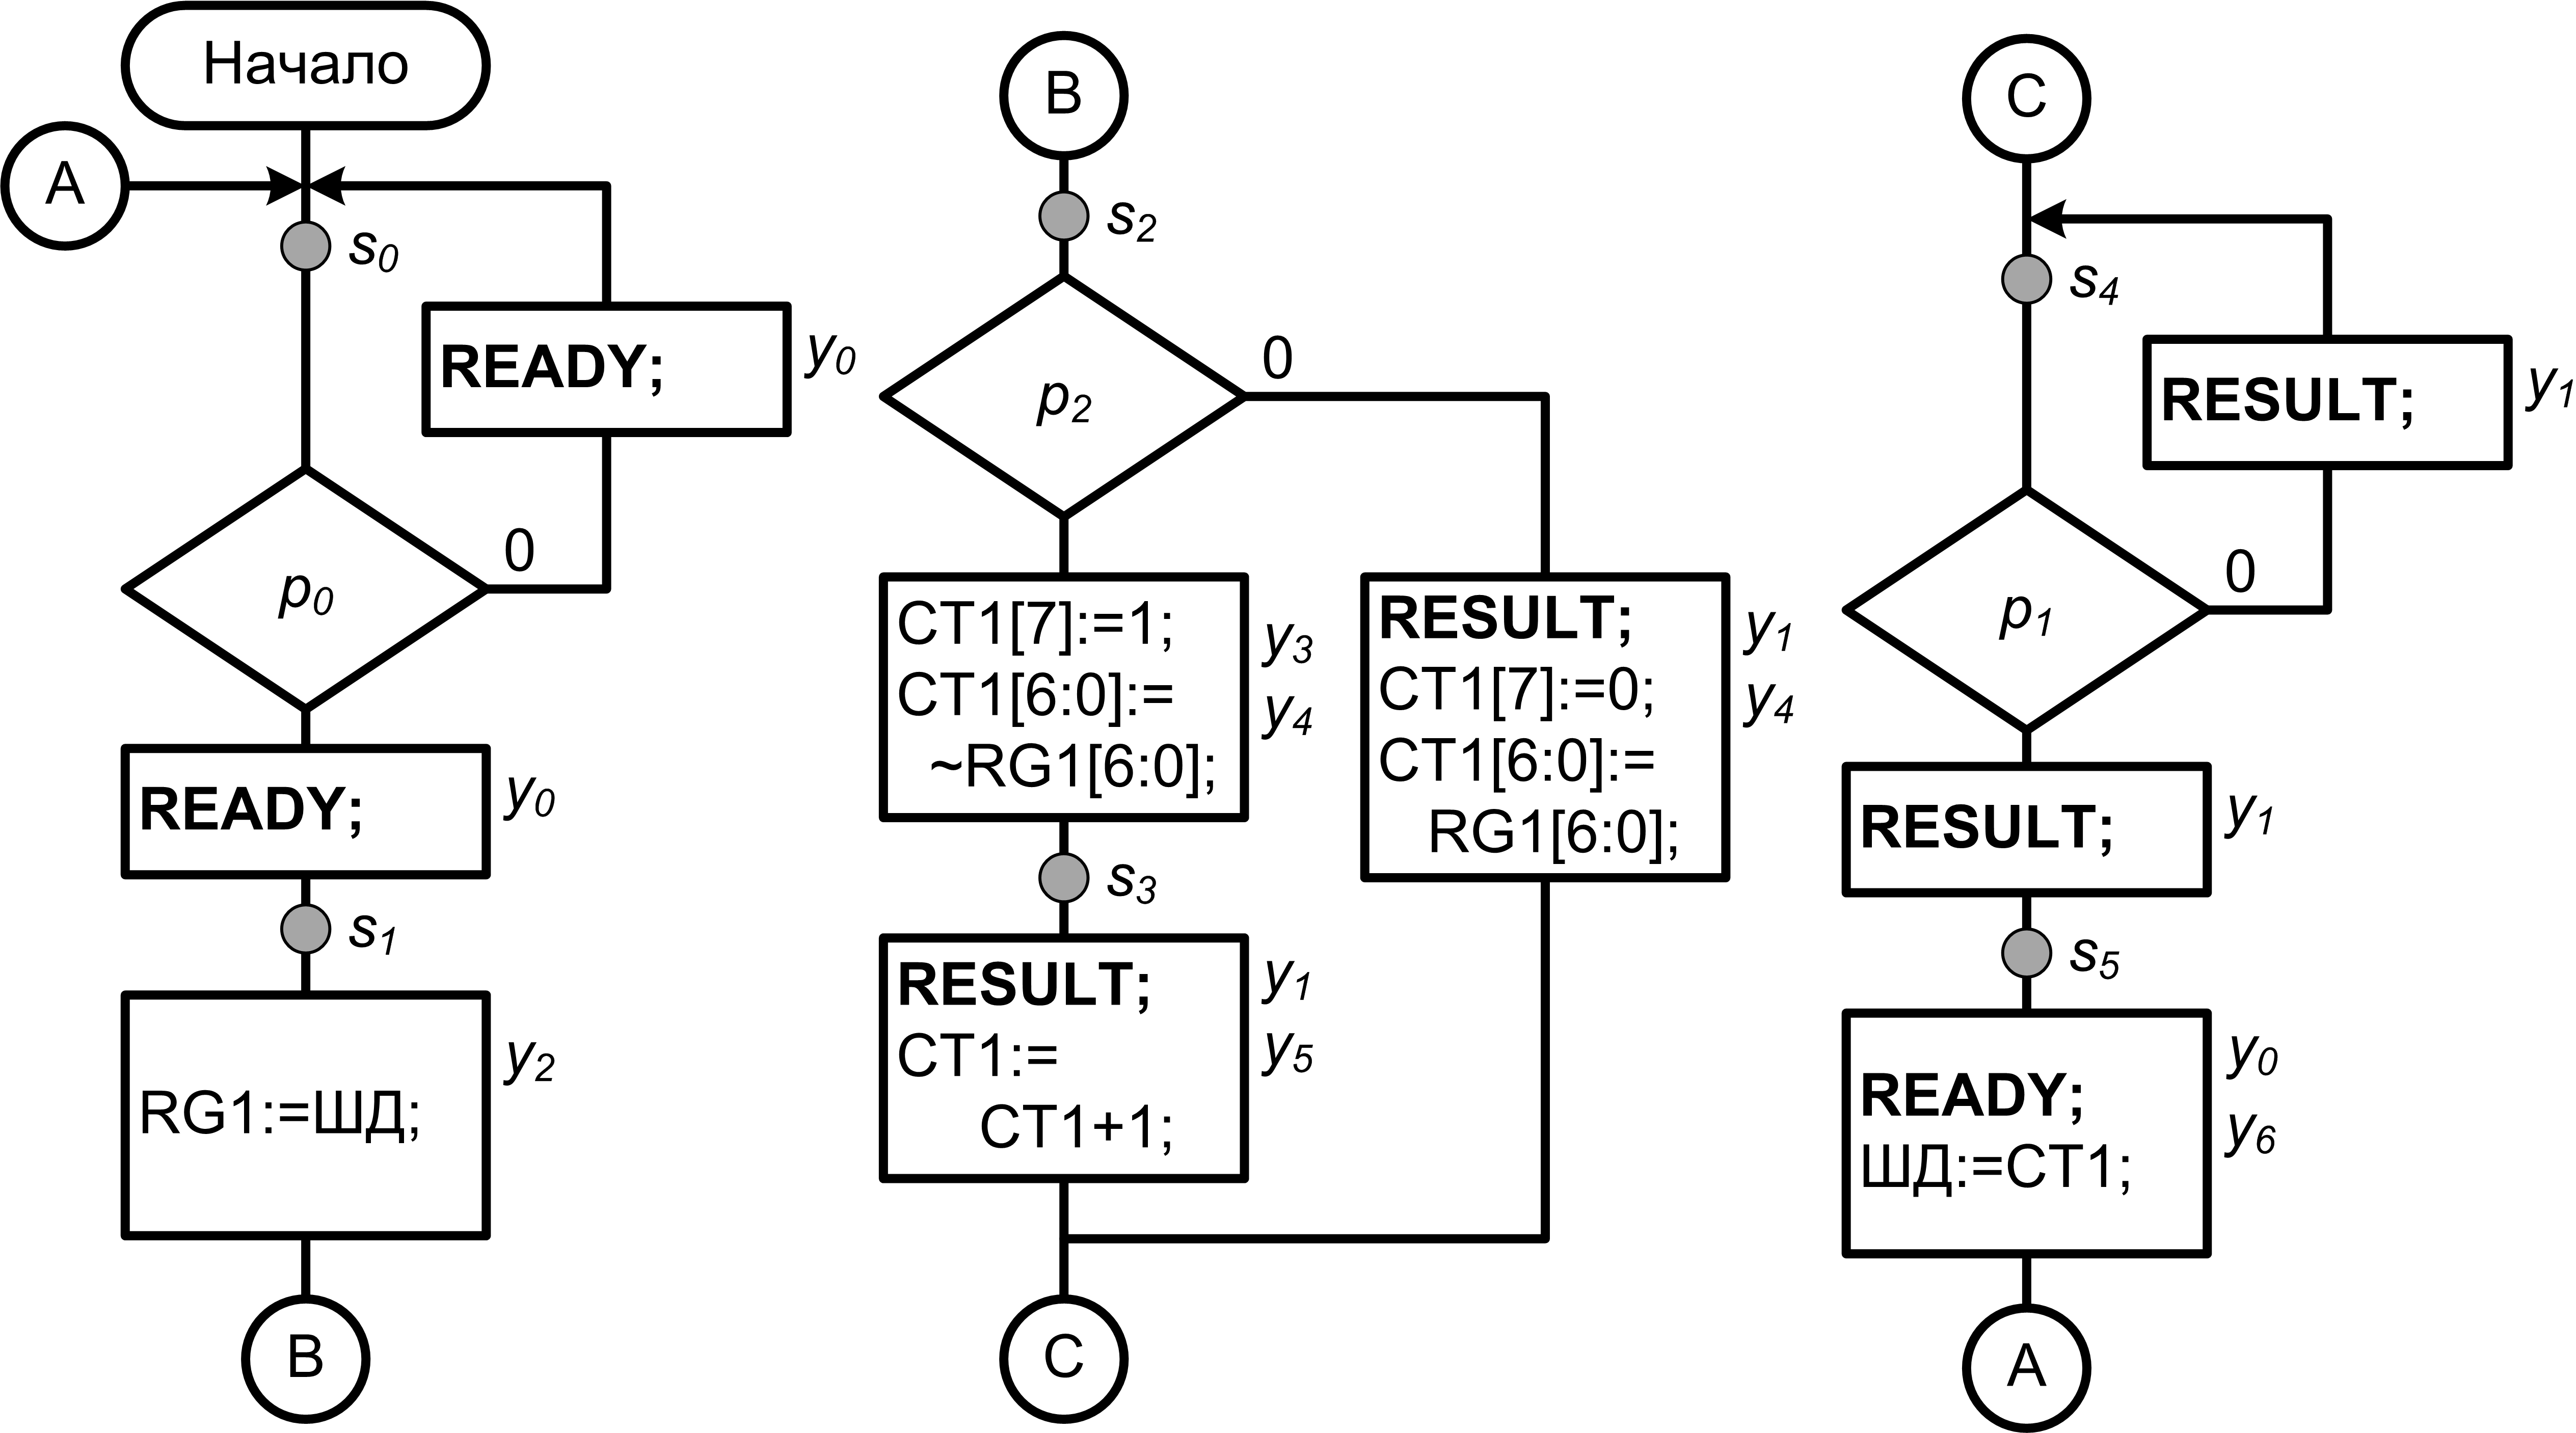
\includegraphics[width=\textwidth]{fig/miliPcDcAlgo}
    \caption{Алгоритм работы преобразователя $\Machine{ПК}\mapsto\Machine{ДК}$ под управлением автомата Мили}
    \label{fig::ch::practice::miliPcDcAlgo}
\end{figure}

Отметка состояния ставится над условной вершиной (см. рисунок \ref{fig::ch::practice::MiliAlg}). При отсутствии таковой, например, между двумя последовательными блоками процеса\footnote{Блок процесса обозначается на блок-схеме прямоугольником}, вводится фиктивная вершина условия с одинаковым исходом для истины и лжи. В данном примере фиктивные условные вершины введены для состояний $s_1$, $s_3$, $s_5$.

Также следует отметить, что сигнал $y_0\Machine{(ACK)}$ (<<Задание принял>>) выдается в следующем такте (при переходе из состояния $s_1$). Автомат мог среагировать на поступивший сигнал $p_0$ в текущем такте и выдать подтверждение приема задания, но это могло привести к гонкам\footnote{Потому что упрвляющий автомат ЦУУ, при поступлении подтверждения приема должен снять сигнал выдачи задания и, если он это сделает в текущем такте, то начнутся гонки сигналов $p_0$ и $y_0$} и нарушению соглашения приема задания, приведенного на рисунке \ref{fig::ch::practice::timingsTr}.

Соответствующая алгоритму диаграмма переходов автомата уже была приведена на рисунке \ref{fig::ch::practice::MiliDiagram}. Теперь несложно задать микропрограмму для автомата (рисунок \ref{fig::ch::practice::miliMcu}). Это можно сделать как по отмеченной граф-схеме, так и по диаграмме переходов.

\begin{figure}[!ht]
    \centering
    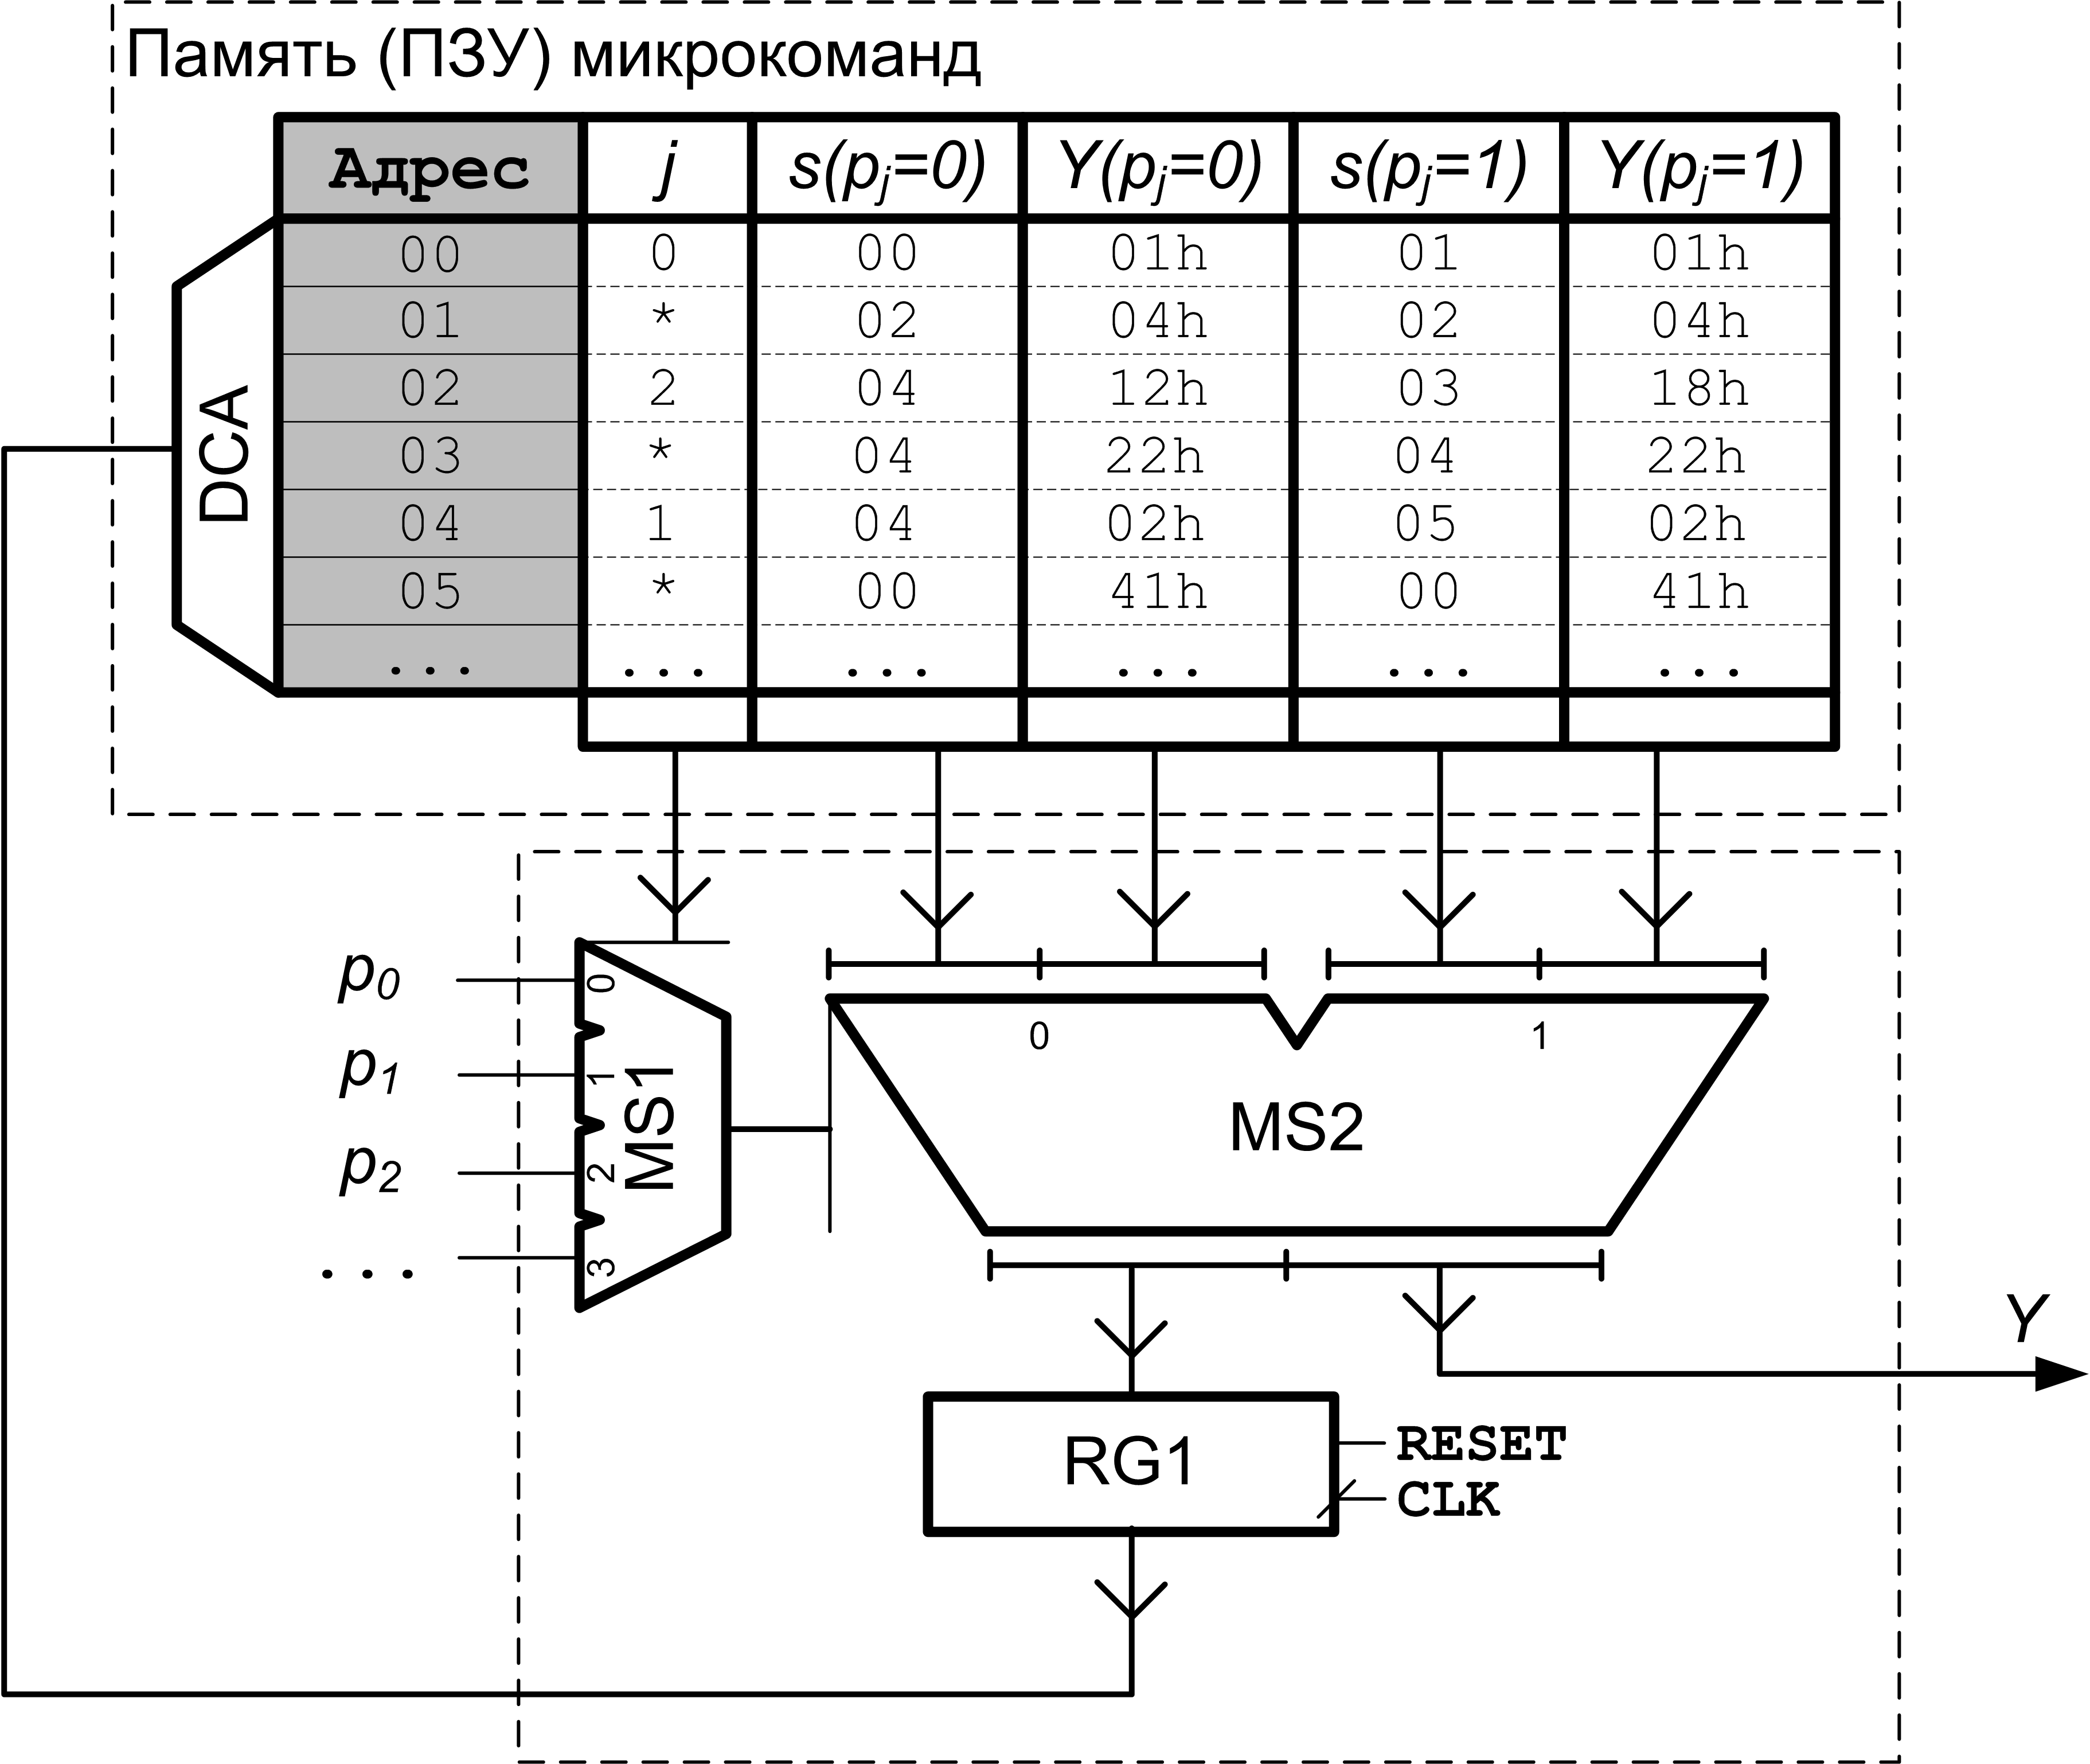
\includegraphics[width=.7\textwidth]{fig/miliMcu}
    \caption{Микропрограмма автомата Мили}
    \label{fig::ch::practice::miliMcu}
\end{figure}

Временная диаграмма работы преобразователя $\Machine{ПК}\mapsto\Machine{ДК}$ под управлением автомата Мили приводится на рисунке \ref{fig::ch::practice::timingsMili}.

\begin{figure}[!ht]
    \centering
    \includegraphics{fig/timings.3}
    \caption{Временная диаграмма работы преобразователя $\Machine{ПК}\mapsto\Machine{ДК}$ под управлением автомата Мили}
    \label{fig::ch::practice::timingsMili}
\end{figure}


\subsubsection{Автомат Мура}

Алгоритм работы преобразователя $\Machine{ПК}\mapsto\Machine{ДК}$, учитывающий особенности управляющего автомата Мура приведен на рисунке \ref{fig::ch::practice::moorePcDcAlgo}.

%todo особенности

\begin{figure}[!ht]
    \centering
    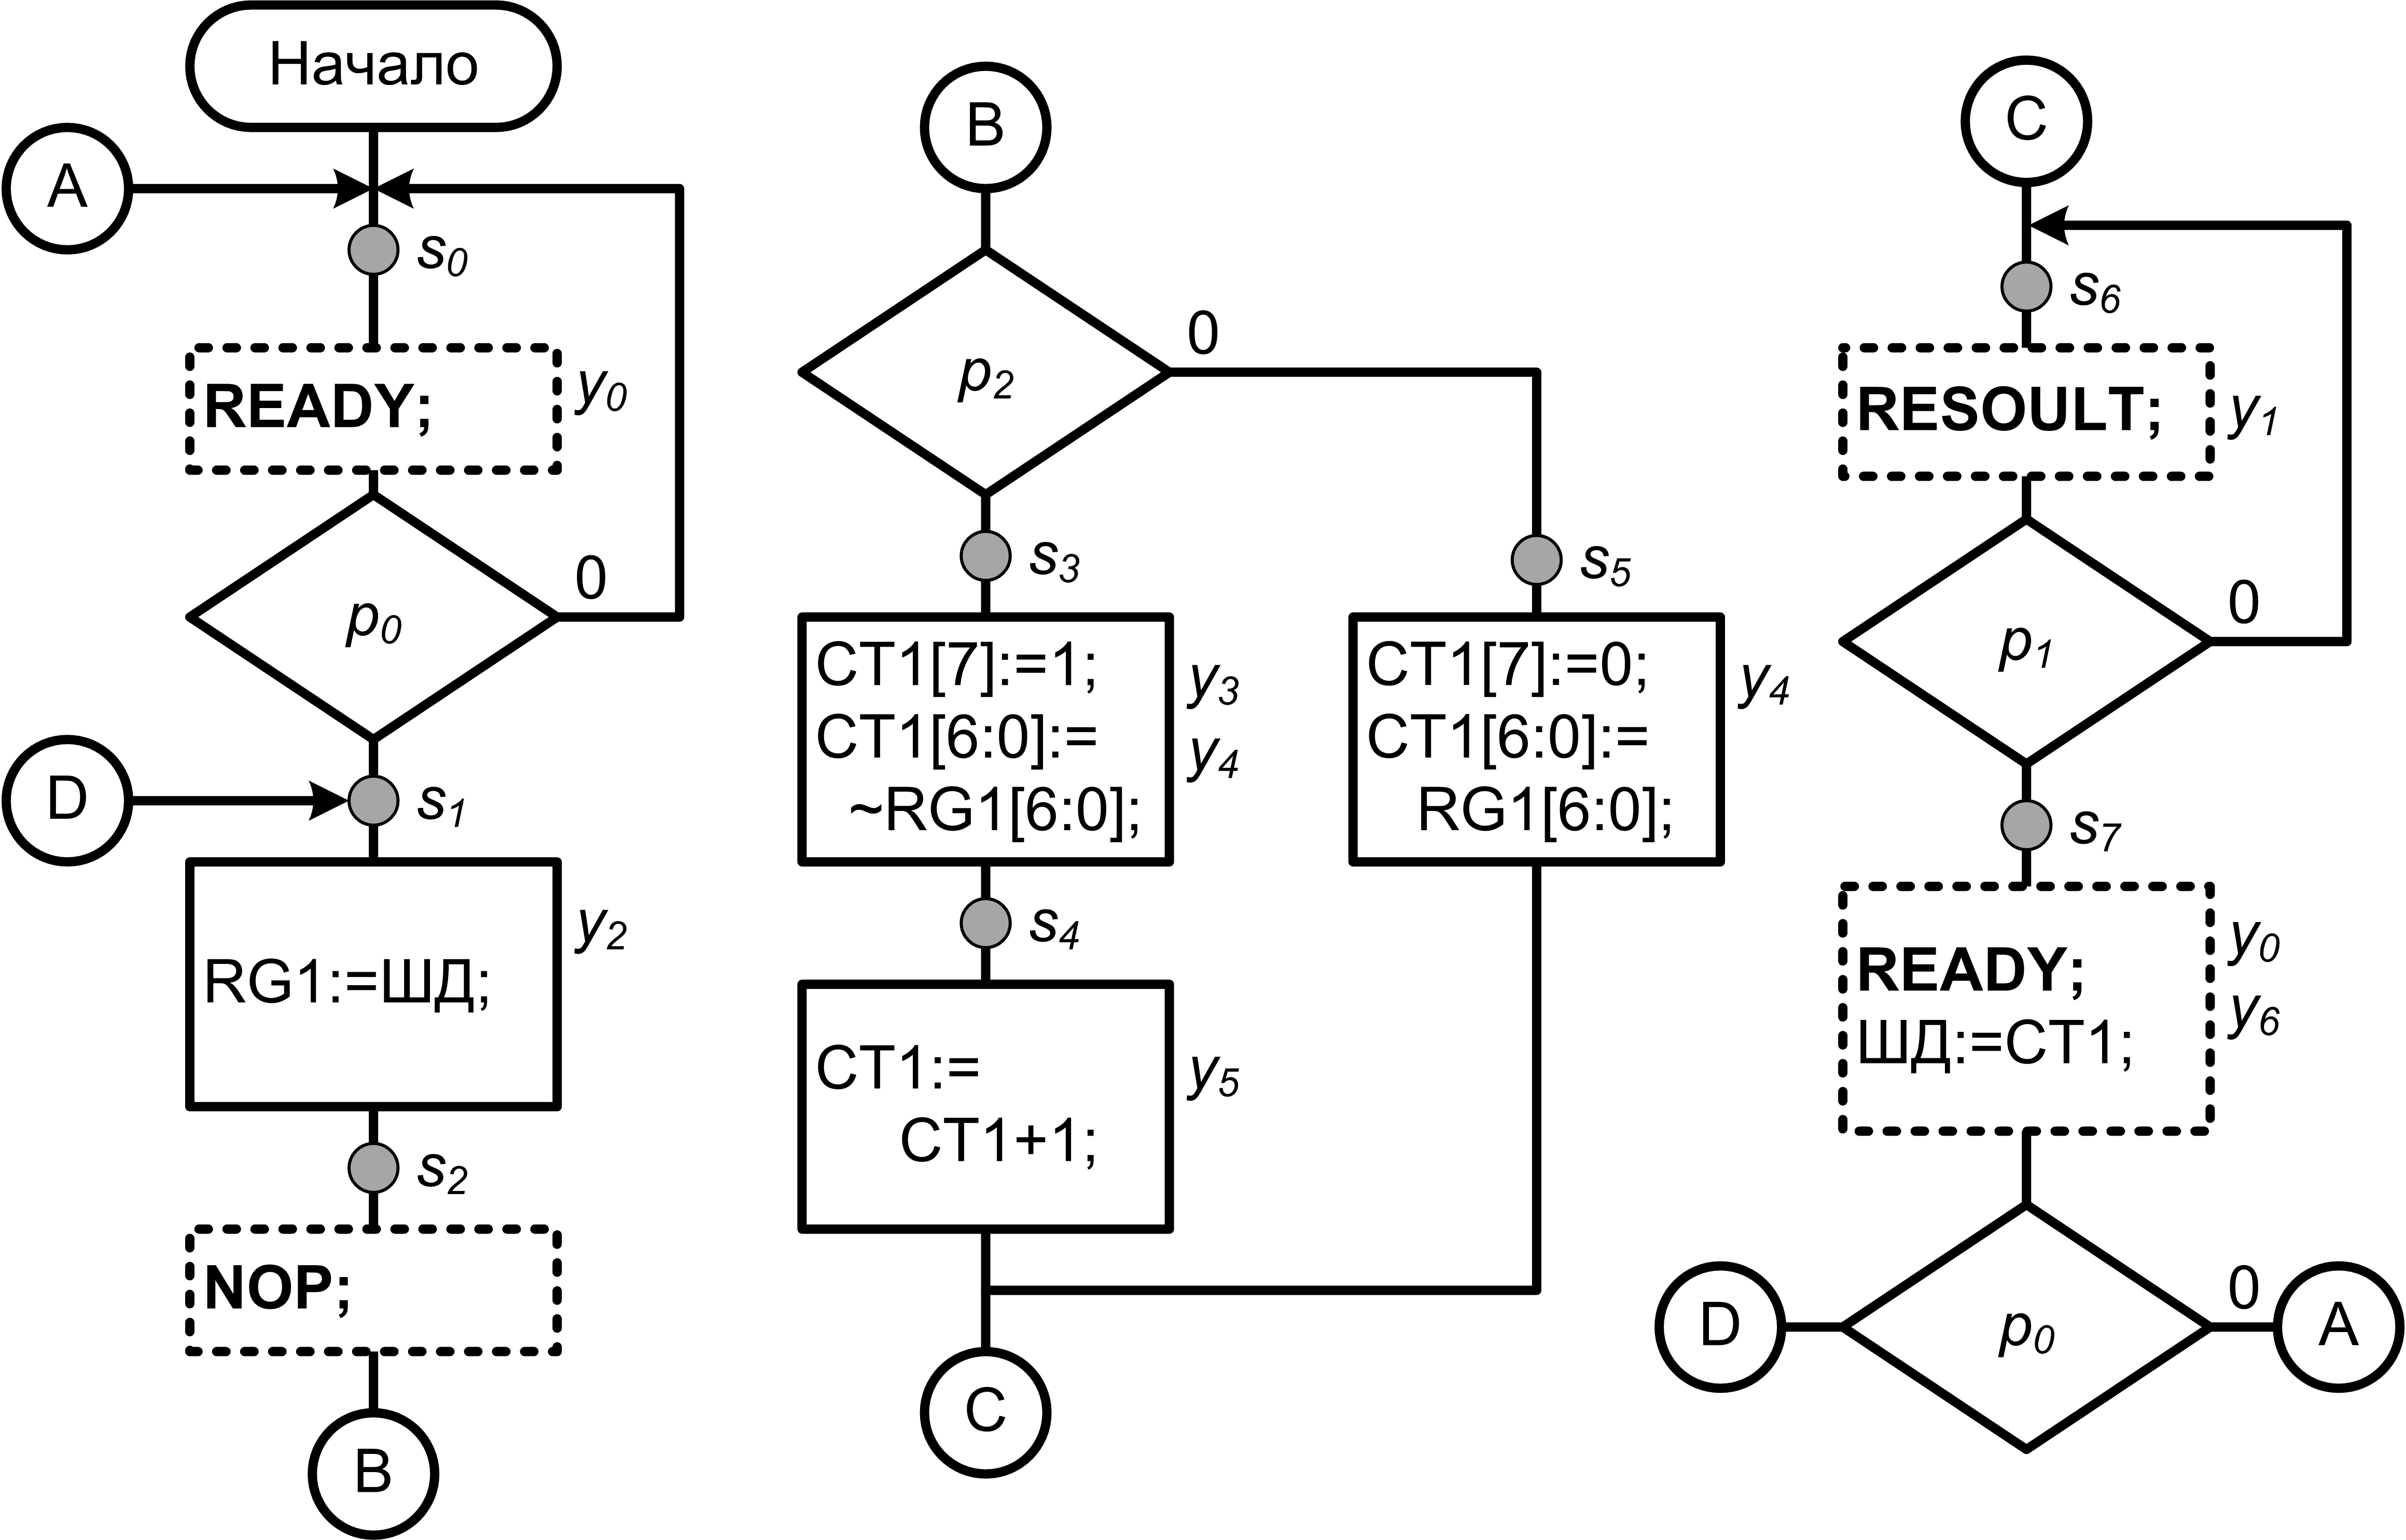
\includegraphics[width=\textwidth]{fig/moorePcDcAlgo}
    \caption{Алгоритм работы преобразователя $\Machine{ПК}\mapsto\Machine{ДК}$ под управлением автомата Мура}
    \label{fig::ch::practice::moorePcDcAlgo}
\end{figure}

Диаграмма состояний автомата Мура уже была приведена на рисунке \ref{fig::ch::practice::MooreDiagram}. Обычно у автомата Мура, эквивалентного автомату Мили, состояний больше, и времени (тактов) на работу он также тратит больше.

Прошивка памяти микропрограммного автомата Мура приводится на рисунке \ref{fig::ch::practice::mooreMcu}.

\begin{figure}[!ht]
    \centering
    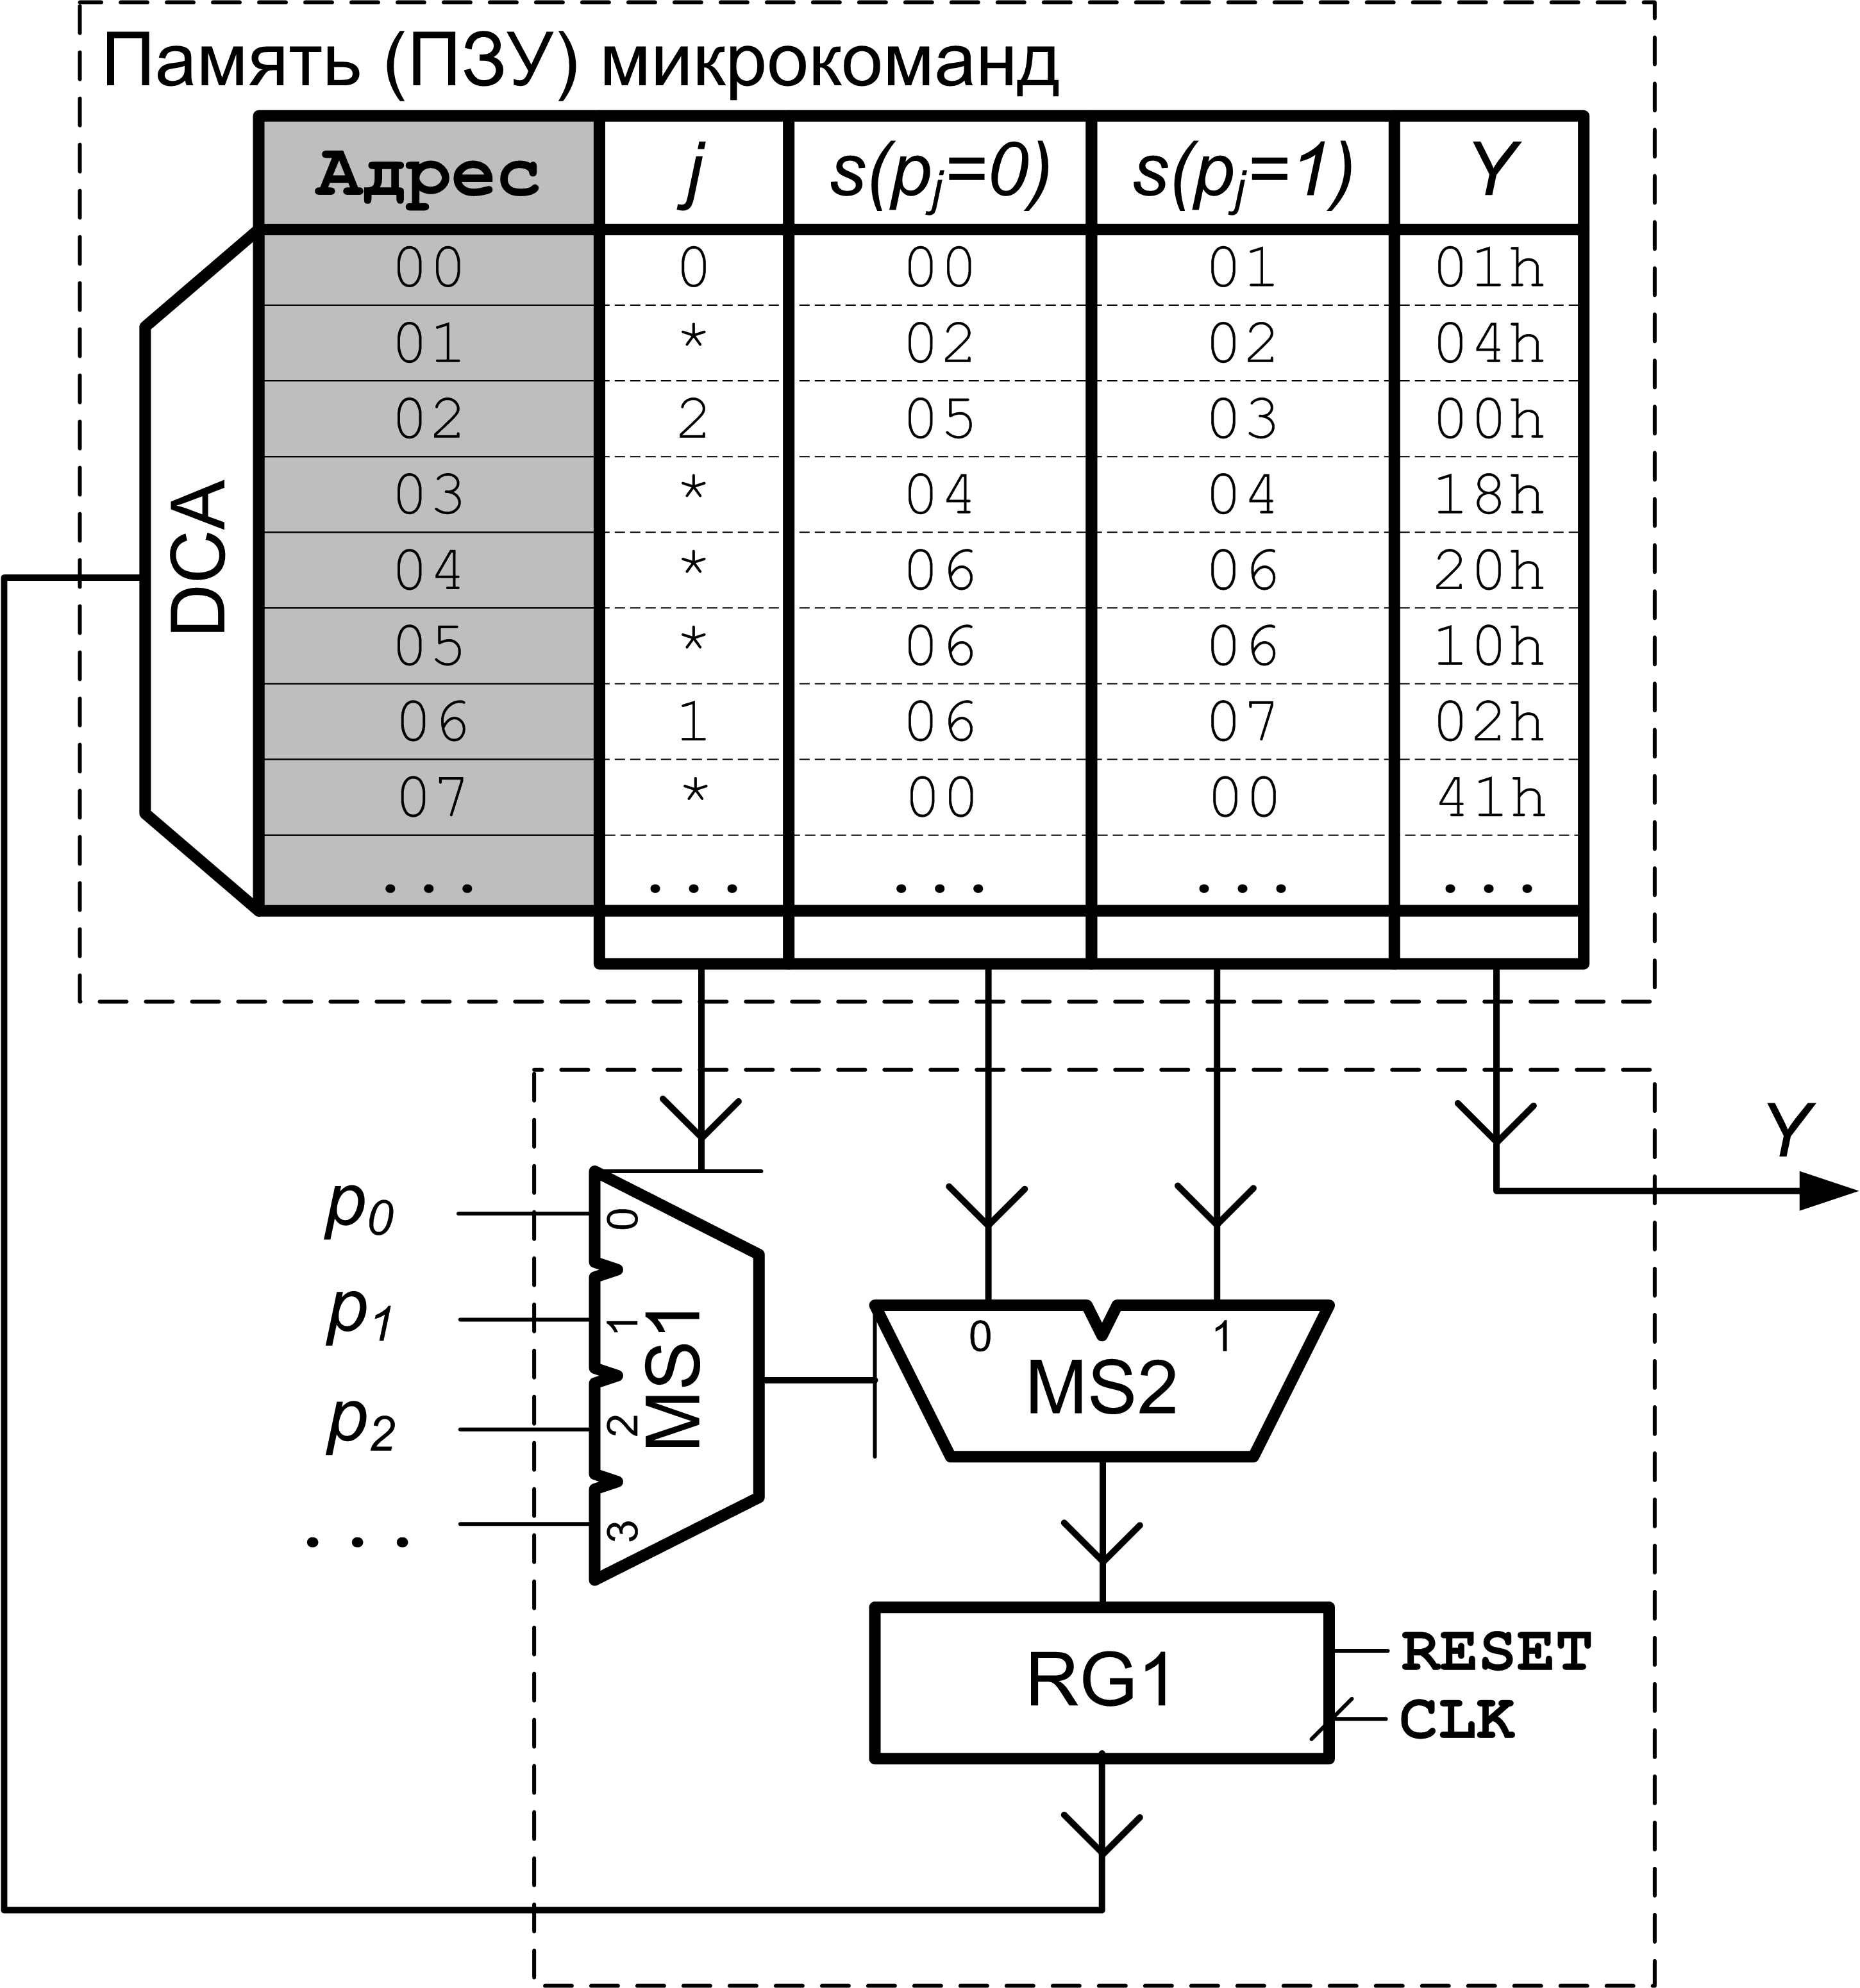
\includegraphics[width=.6\textwidth]{fig/mooreMcu}
    \caption{Микропрограмма автомата Мура}
    \label{fig::ch::practice::mooreMcu}
\end{figure}

Временная диаграмма работы автомата Мура приведена на рисунке \ref{fig::ch::practice::timingsMoore}.

\begin{figure}[!ht]
    \centering
    \includegraphics{fig/timings.4}
    \caption{Временная диаграмма работы преобразователя $\Machine{ПК}\mapsto\Machine{ДК}$ под управлением автомата Мура}
    \label{fig::ch::practice::timingsMoore}
\end{figure}



\section{Работа с лабораторной установкой <<Microcode>>}
\label{s::ch::practice::software}

Цель лабораторной установки <<Microcode>> --- закрепление теоретических основ реализации арифметических операций.

Поставленная цель достигается за счет того, что:
\begin{itemize}
    \item предлагается готовая операционная часть устройства (см. рисунок \ref{fig::ch::practice::model} и теорию в разделе \ref{ch::practice}), в структуре которой требуется разобраться и понять, как имеющимися средствами решить задачу (т.е. выполнить некоторую арифметическую операцию);

    \item моделируется работа центрального управляющего устройства, которое выдает задание и принимает результаты по определенным правилам;

    \item <<Microcode>> позволяет студенту задать собственные входные данные и выполнить пошаговое управление в режиме отладки;
    
    \item <<Microcode>> автоматически выполняет многократное тестирование правильности решения задачи по методу <<черного ящика>>;
    
    \item выполняемые <<Microcode>> тесты покрывают все ветки правильного алгоритма решения задачи (арифметической операции);
    
    \item тесты покрытия создаются <<Microcode>> на основе генератора случайных чисел;
    
    \item в <<Microcode>> заложена возможность генерации индивидуальных вариантов заданий, создаваемых за счет перестановки индексов управляющих сигналов $y$, что порождает $n!$ возможных уникальных вариантов кодирования, при среднем $n\ge 12$;
    
    \item в диалогах <<Microcode>> для ввода отладочных данных автоматически рассчитывается результат, а также выводятся десятичные представления числовых операндов, что дает возмножность глубже разобраться в форматах и кодах.
\end{itemize}


\subsection{Принципы работы <<Microcode>>}

Лабораторная установка <<Microcode>> позволяет загружать групу заданий. Например, в рамках одной группы могут быть загружены задания на умножение чисел различными способами (см. рисунок \ref{fig:mic:MicWindow}).

\begin{figure}
    \centering
    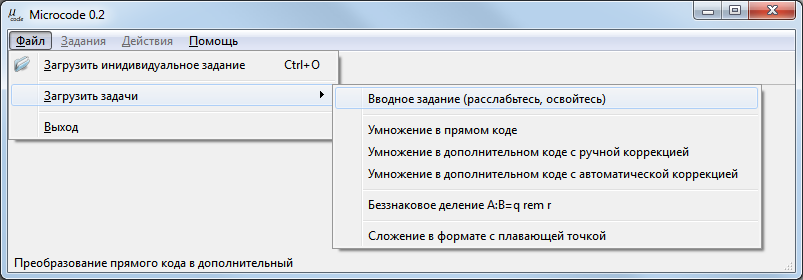
\includegraphics[width=\textwidth]{fig/MicWindow}
    \caption{Главное окно <<Microcode>> (русский язык интерфейса)}\label{fig:mic:MicWindow}
\end{figure}

Отдельное задание представляет собой вычислительное устройство, постороенное в соответствии с принципами, изложенными в разделе \ref{ch::practice} и способное выполнять ту или иную сложную вычислительную операцию, например, умножение или деление.

Пользователю предлагается готовая схема операционной части, в устройстве и назначении которой он должен разобраться, опираясь на изученную теорию. В распоряжении пользователя имеется набор управляющих сигналов, с помощью которых он может изменять состояние операционной части. Задача пользователя --- реализовать алгоритм работы сложной вычислительной операции.

У пользователя имеются следующие возможности реализовать алгоритм работы устройства:
\begin{itemize}
    \item вручную выполнить выдачу необходимых управляющих сигналов, предварительно задав наборы управляющих сигналов в ПЗУ микрокоманд;
    \item запрограммировать автомат Мили или Мура, заполнив таблицу ПЗУ микропрограмм.
\end{itemize}

Все значения в таблицы ПЗУ заносятся в шестнадцатеричной системе счисления. Управляющие сигналы кодируются двоичным вектором, который в ПЗУ вносится в шестнадцатеричном представлении, например, если требуется выдать сигналы $y_5,y_3,y_2,y_0$, то в соответствующей ячейке ПЗУ нужно записать значение \Machine{0x2D}.

По команде пользователя <<Microcode>> выполняет автоматическое тестирование составленного пользователем алгоритма. Чтобы составить корректный алгоритм, пользователь может использовать специальный режим отладки, в котором он может задать исходные данные и в пошаговом режиме отследить изменения, происходящие в операционной части.

Прохождение автоматических тестов является допуском к защите разультатов работы.


\subsection{Задания на лабораторные работы}

В рамках лабораторной работы студент выполняет задание, которое выдает преподаватель.

В лабораторной установке <<Microcode>> реализованы следующие задания: 
\begin{itemize}
    \item перевод прямого кода в дополнительный;
    \item умножение в прямом коде;
    \item умножение в дополнительном коде с ручной коррекцией;
    \item умножение в дополнительном коде с автоматической коррекцией;
    \item беззнаковое деление $A\div B = \DivAnswer{q}{r}$;
    \item сложение в формате с плавающей точкой.
\end{itemize}


\subsection{Выполнение задания}

После выбора группы заданий, становится активным пункт меню <<Задания>>(<<Tasks>>), позволяющий переключаться между заданиями в рамках группы (см. рисунок \ref{fig:mic:MicTaskWindow}). Менять группу заданий в дальнейшем нельзя.

\begin{figure}
    \centering
    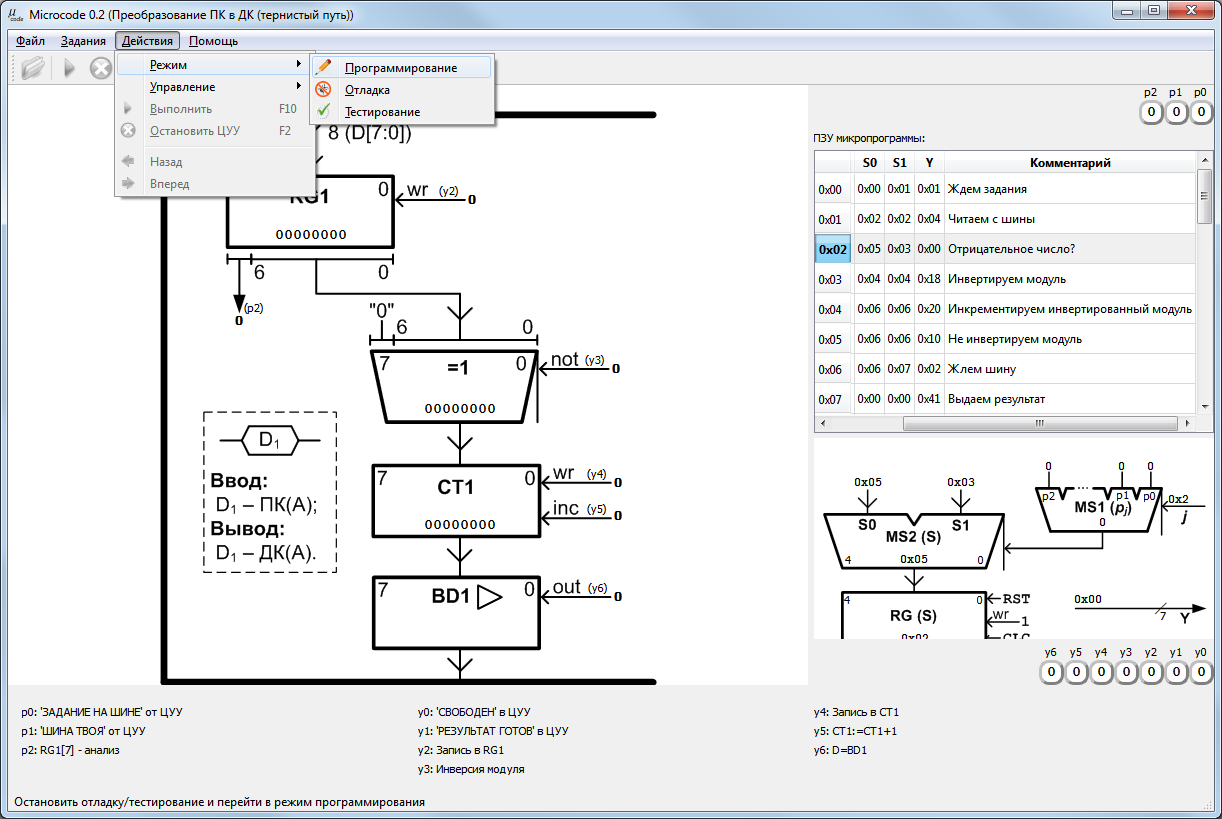
\includegraphics[width=\textwidth]{fig/MicTaskWindow}
    \caption{<<Microcode>> после загрузки заданий}\label{fig:mic:MicTaskWindow}
\end{figure}

Пункт меню <<Действия>> позволяет выполнить те или иные действия в текущем задании:
\begin{itemize}
    \item выбрать один из режимов работы: <<Программирование>> (
\includegraphics[width=16pt]{fig/microcode/image/programming.png}), <<Отладка>> (
\includegraphics[width=16pt]{fig/microcode/image/debug.png}) или <<Тестирование>> (
\includegraphics[width=16pt]{fig/microcode/image/autotest.png});
    \item выбрать управление: <<Ручное>> (
\includegraphics[width=16pt]{fig/microcode/image/manualgun.png}), 
                              <<Автомат Мили>> (
\includegraphics[width=16pt]{fig/microcode/image/miligun.png})
                              или <<Автомат Мура>> (
\includegraphics[width=16pt]{fig/microcode/image/mooregun.png});
    \item выполнять/останавливать шаги отладки или автотесты;
    \item перемещаться в отладочном режиме по истории тактов.
\end{itemize}

Режим работы <<Программирование>> (<<Programming>>) предназначен для редактирования ПЗУ управляющей части. Как только редактирование ячейки ПЗУ завершается, соответствующие управляющие сигналы распространаяются по схеме, но ошибки управления не выдаются, даже если они есть.

Режим <<Отладка>> (<<Debug>>) предназначен для пошагового выполнения придуманного студентом алгоритма управления. В момент переключения в этот режим студенту предлагается ввести исходные данные. После того, как данные будут введены, <<Microcode>> переключается в пошаговый (потактный) режим тестирования. В случае ручного управления (<<Управление/Ручное>> (<<MCU/Manual>>)) пользователь выбирает в таблице <<ПЗУ микрокоманд>> строку с нужной командой и нажимает кнопку <<Выполнить>> (<<Execute>>) или горячую клавишу <<F10>>, что приводит к переключению в следующий такт. В случае автоматического управления (<<Aвтомат Мили>> (<<Mili>>), <<Автомат Мура>> (<<Moore>>)) текущая ячейка ПЗУ микропрограммы (строка таблицы) подсвечивается. Если в процессе выполнения теста фиксируется ошибка, то тестирование прекращается, выводится соответствующее сообщение, и выполняется переход в режим программирования. Если алгоритм выполнен безошибочно и в ЦУУ корректно выдан правильный результат, то выводится информационное сообщение об успешном прохождении отладочного теста.

В режиме <<Тестирование>> (<<Autotest>>) выполняется тестирование на случайным образом генерируемых входных данных. Состояние операционной части при этом не отображается. При ручном управлении автотесты выполняются в пошаговом режиме, в противном случае --- в автоматическом.

В режимах отладки и тестирования фиксируются следующие ошибки, приводящие к прекращению теста:
\begin{itemize}
    \item выполняется чтение данных с <<пустой>> шины;
    \item выполняется выдача данных на <<занятую>> шину;
    \item нарушается протокол взаимодействия с ЦУУ, например, до выдачи результата, выдается сигнал <<Свободен>>;
    \item выдаются конфликтующие сигналы управления элементом памяти, например на регистр одновременно подаются управляющие сигналы сдвига и сброса.
\end{itemize}

Чтобы считать операнды, требуется выполнить следующие действия.
\begin{itemize}
    \item Выдавать сигнал <<Свободен>> ($y_0$, $Y=\Machine{0x0001}$) в течение некоторого числа тактов (не более 6), пока осведомительный сигнал <<Задание на шине>> ($p_0$) не установится в 1.
    \item Сигнал <<Задание на шине>> выдается ЦУУ в течение одного такта, в этом такте также нужно выдавать сигнал <<Свободен>>.
    \item ЦУУ, в течение одного или нескольких тактов, следующих после такта, в котором выдавался сигнал <<Задание на шине>> выдает на шину фрагменты задания. Необходимо считать эти фрагменты в регистры.
\end{itemize}

Чтобы выдать результат, требуется выполнить следующие действия.
\begin{itemize}
    \item Выдавать сигнал <<Результат готов>> ($y_1$, $Y=\Machine{0x0002}$) в течение некоторого числа тактов (не более 6), пока осведомительный сигнал <<Шина твоя>> ($p_0$) не установится в 1.
    \item Сигнал <<Шина твоя>> выдается ЦУУ в течение одного такта, в этом такте также нужно выдавать сигнал <<Результат готов>>.
    \item В течение одного или нескольких тактов, следующих после такта, в котором выдавался сигнал <<Шина твоя>> следует в определенном в задании порядке выдавать фрагменты результата на шину.
\end{itemize}


Результатом работы являются заполненные ПЗУ микрокоманд (ПЗУ микропрограмм). Допуском к защите результатов работы является успешное прохождение студентом отладочных или автоматических тестов.


\subsection{Генерация индивидуальных вариантов заданий}

С помощью microcode можно сгенерировать индивидуальные варианты для каждого студента. Для этих целей нужно сформировать специальный текстовый файл, содержащий список адресатов\footnote{Тех, для кого предназначены индивидуальные варианты заданий. Т.е. студентов.} в формате JSON\footnote{JSON --- JavaScript Object Notation.  Текстовый формат обмена данными, основанный на JavaScript. Прост и лаконичен. Как и многие другие текстовые форматы, JSON легко читается людьми. Формат был разработан Дугласом Крокфордом.}. Файл должен быть сохранен в кодировке UTF-8 и может быть создан в любом подходящем текстовом редакторе.

JSON-содержимое файла адресатов представляет собой массив объектов, состоящих из двух строковых атрибутов:
\begin{itemize}
    \item \verb"id" --- строка, идентифицирующая студента, как правило, содержащая Ф.И.О. студента;
    \item \verb"secret_prefix" --- секретная информация\footnote{В зависимости от степени параноидальности преподавателя, может быть как случайной последовательностью, так и вполне предсказуемой по некоторому, известному только преподавателю, правилу, например, фамилия студента на латинице, или его Ф.И.О., или первые три буквы фамилии\ldots}.
\end{itemize}

Пример содержимого файла адресатов:
\begin{verbatim}
[
    {   "id": "Иванов И.И.",
        "secret_prefix": "IvanovSecret"},
        
    {   "id": "Петров П.П.",
        "secret_prefix": "PetrovSecret"},
        
    {   "id": "Сидоров С.С.",
        "secret_prefix": "SidorovSecret"}
]
\end{verbatim}

После того, как файл подготовлен, можно сгенерировать с помощью microcode индивидуальные варианты. Для этого выполняется пункт меню <<Файл/Создать индивидуальные варианты\ldots>> (<<File/Create individual vatiants\ldots>>). В появившемся диалоге (см. рисунок \ref{fig:mic:genvariants}) следует заполнить необходимые поля.
\begin{itemize}
    \item <<Секрет>>(<<The secret:>>) --- секретная информация, которая используется для проверки подлинности индивидуального варианта. Описание проверки подлинности приводится в разделе \ref{ss:mic:check}.
    
    \item <<Файл с адресатами:>>(<<The recipients file:>>) --- путь к подготовленному файлу адресатов.
    
    \item <<Варианты в папку:>>(<<Variants folder:>>) --- каталог, в котором будут созданы файлы индивидуальных вариантов. Имена файлов будут совпадать со значением атрибута \verb"id" в файле адресатов и иметь расширение <<*.json>>.
\end{itemize}

\begin{figure}[!ht]
    \centering
    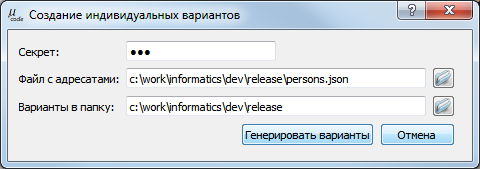
\includegraphics{fig/micvariants}
    \caption{Диалог <<Microcode>> для генерации индивидуальных вариантов (русский язык интерфейса)}\label{fig:mic:genvariants}
\end{figure}

Например, если загрузить приведенный выше файл адресатов, и в качестве секрета ввести <<123>>, то для Иванова будет сгенерирован текстовый файл <<Иванов И.И..json>> со следующим JSON-содержимым:

\begin{verbatim}
{
  "id": "Иванов И.И.",
  "signature": "673e420b...8e76eff8",
  "swap_history": "783590fc...e1c54474"
}
\end{verbatim}

Этот файл может быть загружен в microcode и управляющие сигналы будут перетасованы.


\subsection{Загрузка индивидуального варианта}

После того, как файлы индивидуальных заданий сгенерированы их следует раздать студентам. Индивидуальный вариант загружается студентом командой меню <<Файл/Открыть индивидуальный вариант\ldots>>(<<File/Open individual variant\ldots>>).


\subsection{Проверка подлинности индивидуального варианта}
\label{ss:mic:check}

Файл индивидуального варианта защищен криптографически. Чтобы выполнить проверку подлинности варианта, необходимо выполнить команду меню <<Файл/Проверить индивидуальный вариант\ldots>>(<<File/Validate individual variant\ldots>>).

В диалоге проверки варианта (см. рисунок \ref{fig:mic:checkvarian}) следует ввести конкатенацию секретов $s_1s_2$, где $s_1$ --- секрет, указанный в поле \verb"secret_prefix" файла адресатов, а $s_2$ --- секрет, заданный в диалоге генерации вариантов (см. рисунок \ref{fig:mic:genvariants}).

Для Иванова в приводимых примерах следует ввести: <<IvanovSecret123>>.

\begin{figure}[!ht]
    \centering
    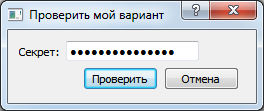
\includegraphics{fig/checkvarian}
    \caption{Диалог <<Microcode>> для проверки подлинности индивидуального варианта (русский язык интерфейса)}\label{fig:mic:checkvarian}
\end{figure}

Без знания секрета, разделенного на две части --- персональную и общую, подделка задания представляет собой вычислительно сложную задачу.

\subsection{Защита результатов работы}

Результаты работы оформляются в виде отчета, в котором для каждого задания необходимо представить:
\begin{itemize}
    \item Таблицы заполненных ПЗУ с построчными комментариями.
    \item Алгоритмы работы управляющего устройства, представленные в виде блок-схемы. Напротив каждого блока процесса должны быть указаны выдаваемые управляющие сигналы.
    \item Таблицы, отражающие пошаговое (потактное) выполнение алгоритма на примере конкретных входных значений.
    \item Выводы в формате формулы изобретения\footnote{Формула изобретения состоит из ограничительной (описательной) и отличительной частей и имеет типовую структуру: <<Изобретение X, состоящее из (список составляющих элементов), отличается тем, что (список отличительных признаков и особенностей)>>. Например, устройство умножения первым способом в прямом коде, реализованное на основе\ldots, отличается тем, что\ldots}. 
    \item Предложения по оптимизации операционной части или микропрограммы.
\end{itemize}

Защищая результаты своей работы, студент должен
\begin{itemize}
    \item \emph{знать}:
    \begin{itemize}
        \item теоретические основы реализуемой в задании вычислительной операции,
        \item принципы работы всех элементов схемы операционной части вычислительного устройства,
        \item протоколы обмена данными с центральным управляющим устройством: <<получение задания>> и <<выдача результата>>;
    \end{itemize}
    \item \emph{уметь}: 
    \begin{itemize}
        \item объяснить, как на предложенной схеме можно реализовать вычислительную операцию (например, в задании умножения в дополнительном коде с ручной коррекцией, указать какие сигналы, в какой последовательности подать, чтобы выполнить коррекцию псевдопроизведения множителем),
        \item кодировать двоичные векторы управляющих сигналов,
        \item реализовать алгоритм вычислительной операции, составляя необходимые наборы микрокоманд или реализуя  микропрограмму,
        \item оценить время выполнения микропрограммы в тактах в зависимости от аргументов: минимальное время, максимальное время, среднее время;
    \end{itemize}
    \item \emph{владеть навыками}:
    \begin{itemize}
        \item перевода двоичных чисел в шестнадцатеричную систему счисления, 
        \item представления чисел в различных форматах, 
        \item составления микропрограмм для автоматов Мили и Мура, 
        \item работы в лабораторной установке <<Microcode>>. 
    \end{itemize}
\end{itemize}


